% DD2350 ADK – Övning 5: Grafalgoritmer och undre gränser
% Kompilera med pdflatex (två gånger). Kräver KTH_logo_RGB_bla.png i samma katalog.
\documentclass[11pt,aspectratio=169,xcolor=table,t]{beamer}
% ---- preamble.tex ----
% ======================================================================
%  PAKET
% ======================================================================
\usepackage[T1]{fontenc}
\usepackage[utf8]{inputenc}
\usepackage[swedish]{babel}
\usepackage{lmodern}
\usepackage[scaled=0.92]{helvet}
\usefonttheme[onlymath]{serif}
\usepackage{amsmath,amssymb,mathtools}
\usepackage{booktabs,tabularx,multirow,array}
\usepackage{pifont}
\usepackage{xspace}
\usepackage{etoolbox}
\usepackage{tikz}
\usetikzlibrary{babel,arrows.meta,positioning,calc,backgrounds,fit,
  decorations.pathreplacing,decorations.pathmorphing,shapes.geometric,
  shapes.misc,shapes.symbols,matrix,patterns,shadows}
\usepackage{tcolorbox}
\tcbuselibrary{skins}
\usepackage[noend]{algpseudocode}

\hypersetup{pdftitle={DD2350 ADK – Övning 5: Grafalgoritmer och undre gränser},
            pdfauthor={Marcus}}

% ======================================================================
%  TEMA  (fristående block — byt gärna mot DD1331-temat)
% ======================================================================
\definecolor{kthblue}{HTML}{004791}
\definecolor{kthnavy}{HTML}{000061}
\definecolor{kthsky}{HTML}{6298D2}
\definecolor{kthlight}{HTML}{DEF0FF}
\definecolor{kthgreen}{HTML}{0D4A21}
\definecolor{kthgrass}{HTML}{4DA061}
\definecolor{kthmint}{HTML}{C7EBBA}
\definecolor{brick}{HTML}{9E1B32}
\definecolor{coral}{HTML}{E86A58}
\definecolor{sand}{HTML}{EFE6D8}
\definecolor{bark}{HTML}{8C6239}
\definecolor{kthorange}{HTML}{E07B00}
\definecolor{lampyellow}{HTML}{FFCC33}
\definecolor{plum}{HTML}{6E3A8C}

\setbeamersize{text margin left=0.6cm,text margin right=0.6cm}
\setbeamertemplate{navigation symbols}{}
\setbeamercolor{normal text}{fg=black!87}
\setbeamercolor{structure}{fg=kthblue}
\setbeamercolor{alerted text}{fg=brick}
\setbeamercolor{frametitle}{fg=kthnavy}
\setbeamercolor{title}{fg=kthnavy}
\setbeamercolor{block title}{bg=kthblue,fg=white}
\setbeamercolor{block body}{bg=kthlight!70}
\setbeamerfont{frametitle}{size=\large,series=\bfseries}
\setbeamerfont{framesubtitle}{size=\small}
\setbeamerfont{footline}{size=\tiny}
\setbeamertemplate{itemize item}{\raisebox{0.12ex}{\color{kthblue}\scriptsize$\blacktriangleright$}}
\setbeamertemplate{itemize subitem}{\color{kthsky}\textbf{--}}
\setbeamertemplate{enumerate item}{\color{kthblue}\bfseries\insertenumlabel.}
\setlength{\leftmargini}{1.2em}

\makeatletter
\setbeamertemplate{frametitle}{%
  \vskip0.30cm
  \begin{minipage}[t]{\dimexpr\textwidth-1.1cm\relax}%
    \usebeamerfont{frametitle}\usebeamercolor[fg]{frametitle}\insertframetitle
    \ifx\insertframesubtitle\@empty\else
      \par\vskip1pt{\usebeamerfont{framesubtitle}\color{kthblue}\insertframesubtitle}\fi
  \end{minipage}\par
  \vskip3pt
  {\color{kthsky}\rule{\textwidth}{0.6pt}}%
  \vskip-1pt}
\makeatother

\newif\ifkthlogo \kthlogotrue
\setbeamertemplate{background}{%
  \ifkthlogo
  \begin{tikzpicture}
    \useasboundingbox (0,0) rectangle (\paperwidth,\paperheight);
    \node[anchor=north east,inner sep=0pt] at (\paperwidth-0.28cm,\paperheight-0.2cm)
      {
\includegraphics[height=0.82cm]{KTH_logo_RGB_bla.png}};
  \end{tikzpicture}%
  \fi}

\setbeamertemplate{footline}{%
  \leavevmode\hbox to\paperwidth{%
    \hskip0.6cm\usebeamerfont{footline}%
    {\color{kthblue}\bfseries DD2350 ADK}\hskip0.5em{\color{kthsky}|}\hskip0.5em
    {\color{black!55}Övning 5\hskip0.5em{\color{kthsky}|}\hskip0.5em\insertsectionhead}%
    \hfill{\color{kthblue}\bfseries\insertframenumber}\hskip0.6cm}%
  \vskip0.2cm}

% ======================================================================
%  IKONER
% ======================================================================
% Kanin (kaninhål = fördjupning som går att hoppa över)
\newcommand{\kaninikon}{\tikz[baseline=0pt,scale=0.125]{%
  \fill[black!75] (0.1,0) ellipse (1.45 and 0.2);
  \fill[bark] (0,0.9) ellipse (0.95 and 0.68);
  \fill[bark] (0.88,1.42) circle (0.45);
  \fill[bark,rotate around={-12:(0.8,1.78)}] (0.72,2.28) ellipse (0.14 and 0.52);
  \fill[bark,rotate around={-38:(1.0,1.78)}] (1.12,2.25) ellipse (0.14 and 0.52);
  \fill[white] (1.03,1.5) circle (0.08);
  \fill[white] (-0.95,1.02) circle (0.24);}}
\newcommand{\kh}{\kaninikon\ \textcolor{bark}{Kaninhål:}\ }
% Varningstriangel
\newcommand{\varningikon}{\tikz[baseline=-0.6ex,scale=0.28]{%
  \fill[brick,rounded corners=0.4pt] (-0.62,-0.5) -- (0.62,-0.5) -- (0,0.6) -- cycle;
  \node[white,font=\bfseries\tiny,inner sep=0] at (0,-0.08) {!};}}
\newcommand{\ja}{\textcolor{kthgrass}{\ding{51}}}
\newcommand{\nej}{\textcolor{brick}{\ding{55}}}

% ======================================================================
%  VARIATIONSTEORI
% ======================================================================
\newcommand{\vtag}[1]{\tikz[baseline=(t.base)]\node[fill=kthgreen,text=white,
  rounded corners=2pt,inner sep=1.6pt,font=\scriptsize\bfseries](t){#1};}
% \varstrip{Mönster}{Fast}{Varierar}{Urskiljs}
\newcommand{\varstrip}[4]{%
  \par\vfill
  \begin{tcolorbox}[enhanced,halign=left,colback=kthmint!40,colframe=kthgreen,boxrule=0.5pt,
     arc=2pt,left=4pt,right=4pt,top=1.5pt,bottom=1.5pt,fontupper=\scriptsize]
  \vtag{#1}\ \textbf{Fast:} #2\enspace\textcolor{kthgreen}{$\cdot$}\enspace
  \textbf{Varierar:} #3\enspace\textcolor{kthgreen}{$\cdot$}\enspace
  \textbf{Urskiljs:} #4
  \end{tcolorbox}}
\newtcolorbox{missbox}[1][]{enhanced,halign=left,colback=coral!12,colframe=brick,boxrule=0.5pt,
  arc=2pt,left=4pt,right=4pt,top=2pt,bottom=2pt,fontupper=\small,
  before upper={\varningikon\ \textbf{\textcolor{brick}{Missuppfattning:}}\ },#1}
\newtcolorbox{ahabox}[1][]{enhanced,halign=left,colback=lampyellow!22,colframe=kthorange,boxrule=0.5pt,
  arc=2pt,left=4pt,right=4pt,top=2pt,bottom=2pt,fontupper=\small,#1}
\newtcolorbox{infobox}[1][]{enhanced,halign=left,colback=kthlight!60,colframe=kthblue,boxrule=0.5pt,
  arc=2pt,left=4pt,right=4pt,top=2pt,bottom=2pt,fontupper=\small,#1}
\newtcolorbox{kaninbox}[1][]{enhanced,halign=left,colback=white,colframe=bark,boxrule=0.5pt,
  arc=2pt,left=4pt,right=4pt,top=2pt,bottom=2pt,fontupper=\small,#1}

% Kaninhålsbilder: omslut ramen med {\kaninbg ... }
\newcommand{\kaninbg}{\setbeamercolor{background canvas}{bg=sand!65}}

% Avsnittsbild med lärandeobjekt och kritiska aspekter
\newcommand{\uppgiftsbild}[4]{%
\begin{frame}
  \vskip0.5cm
  \begin{columns}[T]
  \begin{column}{0.2\textwidth}
    \raggedleft{\fontsize{70}{70}\selectfont\bfseries\color{kthsky}#1}
  \end{column}
  \begin{column}{0.74\textwidth}
    {\Large\bfseries\color{kthnavy}#2}\par\vskip0.35cm
    {\small\textbf{\color{kthgreen}Lärandeobjekt:} #3}\par\vskip0.25cm
    {\small\textbf{\color{kthgreen}Kritiska aspekter} (det vi kommer att variera):}
    \small #4
  \end{column}
  \end{columns}
\end{frame}}

% ======================================================================
%  TIKZ
% ======================================================================
\tikzset{
  onslide/.code args={<#1>#2}{\only<#1>{\pgfkeysalso{#2}}},
  alt/.code args={<#1>#2#3}{\alt<#1>{\pgfkeysalso{#2}}{\pgfkeysalso{#3}}},
  invisible/.style={opacity=0,text opacity=0},
  visible on/.style={alt={#1{}{invisible}}},
  >={Stealth[length=2.2mm,width=1.8mm]},
  % grafer
  gv/.style={circle,draw=kthnavy,fill=white,line width=0.7pt,inner sep=0pt,
             minimum size=5.4mm,font=\small},
  ge/.style={draw=black!45,line width=0.8pt,nodes={text=black!75}},
  gw/.style={font=\scriptsize,inner sep=1pt},
  mst/.style={draw=kthblue,line width=2.6pt,nodes={text=kthblue,font=\scriptsize\bfseries}},
  nyss/.style={draw=kthorange,line width=3pt,nodes={text=kthorange,font=\scriptsize\bfseries}},
  rej/.style={draw=brick!60,line width=0.9pt,dash pattern=on 2.5pt off 1.5pt,nodes={text=brick!70}},
  rejnu/.style={draw=brick,line width=2pt,dash pattern=on 3pt off 1.5pt,nodes={text=brick,font=\scriptsize\bfseries}},
  cand/.style={draw=kthorange,line width=1.5pt,dash pattern=on 3pt off 1.5pt,nodes={text=kthorange,font=\scriptsize\bfseries}},
  faint/.style={draw=black!15,line width=0.6pt,nodes={text=black!35}},
  intree/.style={fill=kthblue,text=white,draw=kthnavy},
  comp1/.style={fill=kthmint,draw=kthgreen},
  comp2/.style={fill=kthlight,draw=kthblue},
  comp3/.style={fill=lampyellow!45,draw=kthorange},
  % flöden
  fn/.style={circle,draw=kthnavy,fill=white,line width=0.7pt,inner sep=0pt,
             minimum size=5.4mm,font=\small},
  fe/.style={->,draw=black!55,line width=0.8pt},
  fl/.style={font=\scriptsize,inner sep=1pt,fill=white,text=black!85,
             rounded corners=1pt},
  res/.style={->,draw=kthblue,line width=0.8pt},
  resb/.style={->,draw=kthorange,line width=0.8pt},
  aug/.style={->,draw=kthgrass,line width=2.4pt},
  sat/.style={->,draw=brick,line width=1.4pt},
  cutline/.style={draw=plum,line width=1.2pt,dash pattern=on 4pt off 2pt},
}

% ======================================================================
%  PSEUDOKOD PÅ SVENSKA
% ======================================================================
\algrenewcommand\algorithmicwhile{\textbf{medan}}
\algrenewcommand\algorithmicdo{\textbf{gör}}
\algrenewcommand\algorithmicfor{\textbf{för}}
\algrenewcommand\algorithmicforall{\textbf{för alla}}
\algrenewcommand\algorithmicif{\textbf{om}}
\algrenewcommand\algorithmicthen{\textbf{så}}
\algrenewcommand\algorithmicelse{\textbf{annars}}
\algrenewcommand\algorithmicreturn{\textbf{returnera}}
\algrenewcommand\algorithmicprocedure{\textbf{procedur}}
\algrenewcommand\algorithmicfunction{\textbf{funktion}}
\algrenewcommand{\algorithmiccomment}[1]{\hfill{\color{black!50}\(\triangleright\) #1}}
\newcommand{\Kw}[1]{\textbf{#1}}

% ======================================================================
%  MATTE
% ======================================================================
\newcommand{\VE}{O(|V|+|E|)}
\newcommand{\absV}{|V|}
\newcommand{\absE}{|E|}

\title{DD2350 ADK – Övning 5: Grafalgoritmer och undre gränser}
\author{Marcus}
\date{HT 2026}
\begin{document}
% ---- s0-intro.tex ----
% ======================================================================
%  INLEDNING
% ======================================================================
\section{Inledning}

{\kthlogofalse
\begin{frame}[plain]
\begin{tikzpicture}[remember picture,overlay]
  \fill[kthlight!55] (current page.north west) rectangle ([xshift=4.6cm]current page.south west);
  \node at ([xshift=2.3cm,yshift=0.35cm]current page.west)
     {
\includegraphics[height=3.1cm]{KTH_logo_RGB_bla.png}};
  \draw[kthsky,line width=1.2pt] ([xshift=4.6cm]current page.north west) -- ([xshift=4.6cm]current page.south west);
  \node[anchor=west,align=left,text width=10cm] at ([xshift=5.3cm,yshift=0.55cm]current page.west) {%
    {\small\color{kthblue}\textsc{DD2350 Algoritmer, datastrukturer och komplexitet}}\\[0.35cm]
    {\fontsize{30}{32}\selectfont\bfseries\color{kthnavy}Övning 5}\\[0.25cm]
    {\Large\color{kthnavy}Grafalgoritmer och undre gränser}\\[0.55cm]
    {\normalsize Marcus \quad{\color{kthsky}|}\quad HT 2026}}; % TODO: namn/titel
  \node[anchor=south west,align=left,text width=10.4cm,font=\tiny,text=black!50]
    at ([xshift=5.3cm,yshift=0.45cm]current page.south west) {%
    Uppgifter och lösningsidéer: Viggo Kann (2026-08-25). Lånade idéer ur tidigare
    övningsbilder: Anton Grensjö (2017), Lisa Li (2019) och Alice.\\
    Sandfärgade bilder med kanin \kaninikon{} är kaninhål: fördjupningar som går att hoppa över.};
\end{tikzpicture}
\end{frame}}

\begin{frame}{Dagens program}
\begin{columns}[T]
\begin{column}{0.55\textwidth}
\begin{enumerate}\setlength{\itemsep}{3pt}
  \item Spännande träd \hfill{\scriptsize\color{black!55}Prim, Kruskal}
  \item Förändrat flöde \hfill{\scriptsize\color{black!55}$\pm1$ på en kant}
  \item Eulercykel \hfill{\scriptsize\color{black!55}linjär tid}
  \item Julklappsfördelning \hfill{\scriptsize\color{black!55}matchning}
  \item Undre gräns för sökning \hfill{\scriptsize\color{black!55}beslutsträd}
  \item Laga julgransbelysning \hfill{\scriptsize\color{black!55}motståndare}
\end{enumerate}
\end{column}
\begin{column}{0.4\textwidth}
\begin{infobox}[fontupper=\footnotesize]
\textbf{Tre sorters bilder}\par\smallskip
\textcolor{kthblue}{\rule[0.2ex]{1.2em}{1.2ex}}\ Lösningar och exempel\par
\textcolor{sand!90!bark}{\rule[0.2ex]{1.2em}{1.2ex}}\ \kaninikon\ Kaninhål (valfria)\par
\textcolor{brick}{\rule[0.2ex]{1.2em}{1.2ex}}\ \varningikon\ Vanliga missuppfattningar\par
\textcolor{kthgreen}{\rule[0.2ex]{1.2em}{1.2ex}}\ \vtag{Kontrast}\ Variationsmönster
\end{infobox}
\end{column}
\end{columns}
\vfill
{\small Övningen gräver ner sig i alla kaninhål. Kaninhålen ligger på egna bilder,
så den som har bråttom kan hoppa över dem. Den som inte har bråttom kan också det.}
\vskip0.2cm
\end{frame}

\begin{frame}{Om upplägget: variationsteori}
\small
\textbf{Idé (Marton):} man urskiljer en aspekt av något först när man upplever att
den \emph{varierar} medan annat hålls fast. Den som bara sett röda bollar vet inte att
bollar har färg.
\medskip
\begin{columns}[T]
\begin{column}{0.49\textwidth}
\begin{itemize}\setlength{\itemsep}{2pt}
  \item \textbf{Lärandeobjekt:} det vi vill att ni ska kunna.
  \item \textbf{Kritiska aspekter:} det man måste urskilja för att kunna det.
  \item Varje uppgift börjar med en bild som säger vilka aspekter vi varierar.
\end{itemize}
\end{column}
\begin{column}{0.49\textwidth}
\footnotesize
\begin{tabular}{@{}l@{\ }p{0.72\linewidth}@{}}
\vtag{Kontrast} & Visa vad det \emph{inte} är (Prim vs Dijkstra).\\[2pt]
\vtag{Separation} & Variera en aspekt, håll resten fast.\\[2pt]
\vtag{Generalisering} & Håll aspekten fast, variera resten.\\[2pt]
\vtag{Fusion} & Variera flera aspekter samtidigt.
\end{tabular}
\end{column}
\end{columns}
\varstrip{Exempel}{grafen}{algoritmen (Prim/Dijkstra)}{att ”girig från en rot” inte säger vad nyckeln är}
\end{frame}

% ---- s1-mst.tex ----
% ======================================================================
%  UPPGIFT 1: SPÄNNANDE TRÄD
% ======================================================================
\section{1 Spännande träd}

\uppgiftsbild{1}{Spännande träd}
{köra Prim och Kruskal för hand — och se \emph{varför} två olika giriga val båda blir rätt.}
{\begin{itemize}\setlength{\itemsep}{1pt}
  \item Kandidatmängden: \emph{hela grafen} (Kruskal) eller \emph{kanten ut ur trädet} (Prim).
  \item Tillståndet under körningen: skog eller träd.
  \item Vad MST beror på: bara vikternas \emph{ordning} (kontrast: kortaste väg).
\end{itemize}}

\begin{frame}{Uppgift 1: Spännande träd}
\begin{columns}[T]
\begin{column}{0.44\textwidth}
\centering
% ---- gen/graf-ren.tex ----
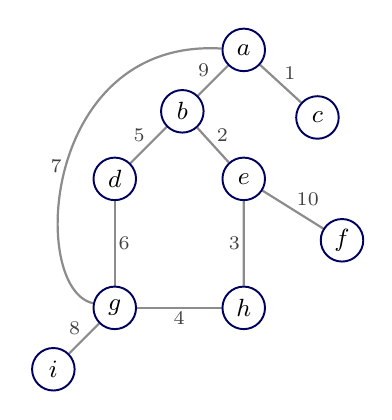
\begin{tikzpicture}[scale=0.78]
  \node[gv] (a) at (3.1,5.2) {$a$};
  \node[gv] (b) at (2.1,4.2) {$b$};
  \node[gv] (c) at (4.3,4.1) {$c$};
  \node[gv] (d) at (1.0,3.1) {$d$};
  \node[gv] (e) at (3.1,3.1) {$e$};
  \node[gv] (f) at (4.7,2.1) {$f$};
  \node[gv] (g) at (1.0,1.0) {$g$};
  \node[gv] (h) at (3.1,1.0) {$h$};
  \node[gv] (i) at (0.0,0.0) {$i$};
  \begin{scope}[on background layer]
  \draw[ge] (a) -- node[gw,above right]{1} (c);
  \draw[ge] (b) -- node[gw,above right]{2} (e);
  \draw[ge] (e) -- node[gw,left]{3} (h);
  \draw[ge] (g) -- node[gw,below]{4} (h);
  \draw[ge] (b) -- node[gw,above left]{5} (d);
  \draw[ge] (d) -- node[gw,right]{6} (g);
  \draw[ge] (a) .. controls (-0.2,5.4) and (-0.4,1.3) .. node[gw,left,pos=0.5]{7} (g);
  \draw[ge] (g) -- node[gw,above left]{8} (i);
  \draw[ge] (a) -- node[gw,above left]{9} (b);
  \draw[ge] (e) -- node[gw,above right]{10} (f);
  \end{scope}
\end{tikzpicture}

\end{column}
\begin{column}{0.53\textwidth}
\begin{infobox}
Visa hur ett minimalt spännande träd hittas i grafen med både \textbf{Prims} och
\textbf{Kruskals} algoritmer.
\end{infobox}
\small
\begin{itemize}\setlength{\itemsep}{3pt}
  \item \textbf{Spännande träd:} delgraf som är ett träd och når \emph{alla} hörn.
        Alltså exakt $|V|-1$ kanter; här $9-1=8$.
  \item \textbf{Minimalt:} minsta möjliga summa av kantvikterna.
  \item Båda algoritmerna är \emph{giriga}. De är bara giriga på olika saker.
\end{itemize}
\end{column}
\end{columns}
\end{frame}

\begin{frame}{Två giriga algoritmer — och en minnesregel}
\begin{columns}[T]
\begin{column}{0.49\textwidth}
\begin{infobox}[title={\textbf{Kruskal}},coltitle=white,colbacktitle=kthblue,fonttitle=\small,
  toptitle=1pt,bottomtitle=1pt]
Ta den \textbf{globalt} billigaste kanten, i hela grafen, som förbinder två
\emph{olika komponenter}. Tillståndet är en \emph{skog}.
\end{infobox}
\end{column}
\begin{column}{0.49\textwidth}
\begin{infobox}[title={\textbf{Prim}},coltitle=white,colbacktitle=kthblue,fonttitle=\small,
  toptitle=1pt,bottomtitle=1pt]
Ta den billigaste kanten som går \textbf{ut ur trädet}. Tillståndet är ett enda
\emph{träd} som växer från en rot.
\end{infobox}
\end{column}
\end{columns}
\medskip
\begin{center}
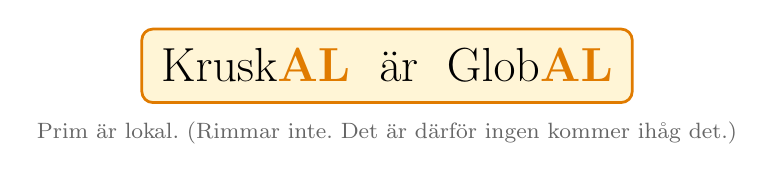
\begin{tikzpicture}
  \node[draw=kthorange,line width=1pt,fill=lampyellow!20,rounded corners=4pt,inner sep=7pt,
        font=\LARGE] (m) {Krusk\textcolor{kthorange}{\textbf{AL}}\ \ är\ \ Glob\textcolor{kthorange}{\textbf{AL}}};
  \node[font=\footnotesize,text=black!60,below=3pt of m]
     {Prim är lokal. (Rimmar inte. Det är därför ingen kommer ihåg det.)};
\end{tikzpicture}
\end{center}
\varstrip{Kontrast}{grafen, girigheten}{kandidatmängden}{global kantlista mot lokal snittkant}
\end{frame}

\begin{frame}{Pseudokod}
\begin{columns}[T]
\begin{column}{0.48\textwidth}
{\small\bfseries\color{kthnavy}Kruskal$(G,w)$}
\footnotesize
\begin{algorithmic}[1]
\State $T\gets\emptyset$
\ForAll{$v\in V$} \State \textsc{MakeSet}$(v)$ \EndFor
\State sortera $E$ i växande vikt
\ForAll{$(u,v)\in E$ i sorterad ordning}
  \If{$\textsc{Find}(u)\neq\textsc{Find}(v)$}
    \State $T\gets T\cup\{(u,v)\}$
    \State \textsc{Union}$(u,v)$
  \EndIf
\EndFor
\State \Return $T$
\end{algorithmic}
\end{column}
\begin{column}{0.5\textwidth}
{\small\bfseries\color{kthnavy}Prim$(G,w,r)$}
\footnotesize
\begin{algorithmic}[1]
\ForAll{$v\in V$} \State $\mathit{key}[v]\gets\infty$;\ $\pi[v]\gets\textsc{nil}$ \EndFor
\State $\mathit{key}[r]\gets0$
\State $Q\gets V$ \Comment{prioritet $\mathit{key}$}
\While{$Q\neq\emptyset$}
  \State $u\gets\textsc{ExtractMin}(Q)$
  \ForAll{$(u,v)\in E$}
    \If{\colorbox{lampyellow!50}{$v\in Q$} \textbf{och} $w(u,v)<\mathit{key}[v]$}
      \State $\pi[v]\gets u$;\ $\mathit{key}[v]\gets w(u,v)$ 
    \EndIf
  \EndFor
\EndWhile
\State \Return $\{(\pi[v],v) : v\neq r\}$
\end{algorithmic}
\end{column}
\end{columns}
\vfill
\begin{missbox}
”Villkoret $v\in Q$ är en detalj.” Utan det kan ett redan utplockat hörn få ny nyckel
och ny förälder — och då är resultatet inte längre ett träd. (Just den buggen finns i
äldre övningsbilder.)
\end{missbox}
\end{frame}

% ---- gen/kruskal.tex ----
\begin{frame}{Kruskal på uppgiftens graf}
\begin{columns}[T]
\begin{column}{0.47\textwidth}
\centering
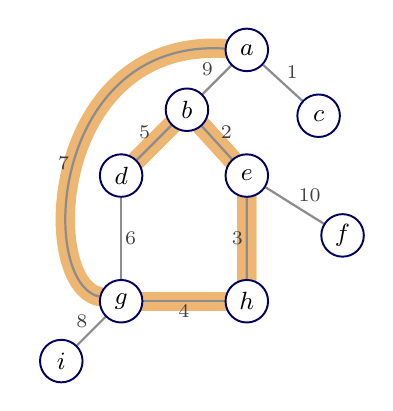
\begin{tikzpicture}[scale=0.76]
  \node[gv,onslide=<2-7>{comp1},onslide=<8->{comp2}] (a) at (3.1,5.2) {$a$};
  \node[gv,onslide=<3->{comp2}] (b) at (2.1,4.2) {$b$};
  \node[gv,onslide=<2-7>{comp1},onslide=<8->{comp2}] (c) at (4.3,4.1) {$c$};
  \node[gv,onslide=<6->{comp2}] (d) at (1.0,3.1) {$d$};
  \node[gv,onslide=<3->{comp2}] (e) at (3.1,3.1) {$e$};
  \node[gv,onslide=<11->{comp2}] (f) at (4.7,2.1) {$f$};
  \node[gv,onslide=<5->{comp2}] (g) at (1.0,1.0) {$g$};
  \node[gv,onslide=<4->{comp2}] (h) at (3.1,1.0) {$h$};
  \node[gv,onslide=<9->{comp2}] (i) at (0.0,0.0) {$i$};
  \begin{scope}[on background layer]
  \draw[kthorange!55,line width=7pt,line cap=round,visible on=<7>] (h) -- (g);
  \draw[kthorange!55,line width=7pt,line cap=round,visible on=<7>] (e) -- (h);
  \draw[kthorange!55,line width=7pt,line cap=round,visible on=<7>] (b) -- (e);
  \draw[kthorange!55,line width=7pt,line cap=round,visible on=<7>] (d) -- (b);
  \draw[kthorange!55,line width=7pt,line cap=round,visible on=<10>] (e) -- (b);
  \draw[kthorange!55,line width=7pt,line cap=round,visible on=<10>] (h) -- (e);
  \draw[kthorange!55,line width=7pt,line cap=round,visible on=<10>] (g) -- (h);
  \draw[kthorange!55,line width=7pt,line cap=round,visible on=<10>] (a) .. controls (-0.2,5.4) and (-0.4,1.3) .. (g);
  \draw[ge,onslide=<2>{nyss},onslide=<3->{mst}] (a) -- node[gw,above right]{1} (c);
  \draw[ge,onslide=<3>{nyss},onslide=<4->{mst}] (b) -- node[gw,above right]{2} (e);
  \draw[ge,onslide=<4>{nyss},onslide=<5->{mst}] (e) -- node[gw,left]{3} (h);
  \draw[ge,onslide=<5>{nyss},onslide=<6->{mst}] (g) -- node[gw,below]{4} (h);
  \draw[ge,onslide=<6>{nyss},onslide=<7->{mst}] (b) -- node[gw,above left]{5} (d);
  \draw[ge,onslide=<7>{rejnu},onslide=<8->{rej}] (d) -- node[gw,right]{6} (g);
  \draw[ge,onslide=<8>{nyss},onslide=<9->{mst}] (a) .. controls (-0.2,5.4) and (-0.4,1.3) .. node[gw,left,pos=0.5]{7} (g);
  \draw[ge,onslide=<9>{nyss},onslide=<10->{mst}] (g) -- node[gw,above left]{8} (i);
  \draw[ge,onslide=<10>{rejnu},onslide=<11->{rej}] (a) -- node[gw,above left]{9} (b);
  \draw[ge,onslide=<11->{nyss}] (e) -- node[gw,above right]{10} (f);
  \end{scope}
\end{tikzpicture}
\end{column}
\begin{column}{0.5\textwidth}
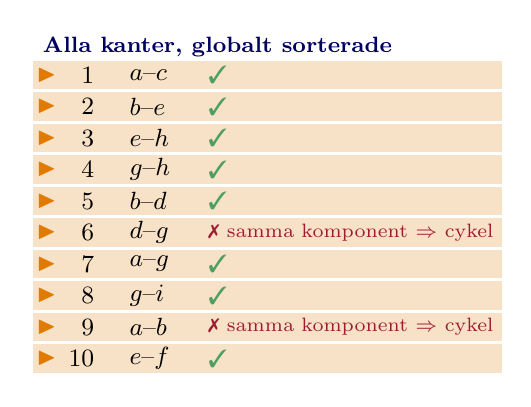
\begin{tikzpicture}[x=1cm,y=-0.40cm,font=\small]
  \node[anchor=west,font=\footnotesize\bfseries,text=kthnavy] at (-0.35,-0.9) {Alla kanter, globalt sorterade};
  \fill[kthorange!22,visible on=<2>] (-0.35,0-0.45) rectangle (5.6,0+0.45);
  \node[visible on=<2>,text=kthorange] at (-0.18,0) {$\blacktriangleright$};
  \node[anchor=east] at (0.55,0) {1};
  \node[anchor=west] at (0.75,0) {$a$--$c$};
  \node[anchor=west,visible on=<2->] at (1.75,0) {\ja};
  \fill[kthorange!22,visible on=<3>] (-0.35,1-0.45) rectangle (5.6,1+0.45);
  \node[visible on=<3>,text=kthorange] at (-0.18,1) {$\blacktriangleright$};
  \node[anchor=east] at (0.55,1) {2};
  \node[anchor=west] at (0.75,1) {$b$--$e$};
  \node[anchor=west,visible on=<3->] at (1.75,1) {\ja};
  \fill[kthorange!22,visible on=<4>] (-0.35,2-0.45) rectangle (5.6,2+0.45);
  \node[visible on=<4>,text=kthorange] at (-0.18,2) {$\blacktriangleright$};
  \node[anchor=east] at (0.55,2) {3};
  \node[anchor=west] at (0.75,2) {$e$--$h$};
  \node[anchor=west,visible on=<4->] at (1.75,2) {\ja};
  \fill[kthorange!22,visible on=<5>] (-0.35,3-0.45) rectangle (5.6,3+0.45);
  \node[visible on=<5>,text=kthorange] at (-0.18,3) {$\blacktriangleright$};
  \node[anchor=east] at (0.55,3) {4};
  \node[anchor=west] at (0.75,3) {$g$--$h$};
  \node[anchor=west,visible on=<5->] at (1.75,3) {\ja};
  \fill[kthorange!22,visible on=<6>] (-0.35,4-0.45) rectangle (5.6,4+0.45);
  \node[visible on=<6>,text=kthorange] at (-0.18,4) {$\blacktriangleright$};
  \node[anchor=east] at (0.55,4) {5};
  \node[anchor=west] at (0.75,4) {$b$--$d$};
  \node[anchor=west,visible on=<6->] at (1.75,4) {\ja};
  \fill[kthorange!22,visible on=<7>] (-0.35,5-0.45) rectangle (5.6,5+0.45);
  \node[visible on=<7>,text=kthorange] at (-0.18,5) {$\blacktriangleright$};
  \node[anchor=east] at (0.55,5) {6};
  \node[anchor=west] at (0.75,5) {$d$--$g$};
  \node[anchor=west,visible on=<7->,font=\scriptsize,text=brick] at (1.75,5) {\nej\ samma komponent $\Rightarrow$ cykel};
  \fill[kthorange!22,visible on=<8>] (-0.35,6-0.45) rectangle (5.6,6+0.45);
  \node[visible on=<8>,text=kthorange] at (-0.18,6) {$\blacktriangleright$};
  \node[anchor=east] at (0.55,6) {7};
  \node[anchor=west] at (0.75,6) {$a$--$g$};
  \node[anchor=west,visible on=<8->] at (1.75,6) {\ja};
  \fill[kthorange!22,visible on=<9>] (-0.35,7-0.45) rectangle (5.6,7+0.45);
  \node[visible on=<9>,text=kthorange] at (-0.18,7) {$\blacktriangleright$};
  \node[anchor=east] at (0.55,7) {8};
  \node[anchor=west] at (0.75,7) {$g$--$i$};
  \node[anchor=west,visible on=<9->] at (1.75,7) {\ja};
  \fill[kthorange!22,visible on=<10>] (-0.35,8-0.45) rectangle (5.6,8+0.45);
  \node[visible on=<10>,text=kthorange] at (-0.18,8) {$\blacktriangleright$};
  \node[anchor=east] at (0.55,8) {9};
  \node[anchor=west] at (0.75,8) {$a$--$b$};
  \node[anchor=west,visible on=<10->,font=\scriptsize,text=brick] at (1.75,8) {\nej\ samma komponent $\Rightarrow$ cykel};
  \fill[kthorange!22,visible on=<11>] (-0.35,9-0.45) rectangle (5.6,9+0.45);
  \node[visible on=<11>,text=kthorange] at (-0.18,9) {$\blacktriangleright$};
  \node[anchor=east] at (0.55,9) {10};
  \node[anchor=west] at (0.75,9) {$e$--$f$};
  \node[anchor=west,visible on=<11->] at (1.75,9) {\ja};
\end{tikzpicture}

\vskip2pt
{\footnotesize\color{kthblue}\only<1>{Komponenter: 9\quad Kanter i $T$: 0\quad Vikt: 0}\only<2>{Komponenter: 8\quad Kanter i $T$: 1\quad Vikt: 1}\only<3>{Komponenter: 7\quad Kanter i $T$: 2\quad Vikt: 3}\only<4>{Komponenter: 6\quad Kanter i $T$: 3\quad Vikt: 6}\only<5>{Komponenter: 5\quad Kanter i $T$: 4\quad Vikt: 10}\only<6>{Komponenter: 4\quad Kanter i $T$: 5\quad Vikt: 15}\only<7>{Komponenter: 4\quad Kanter i $T$: 5\quad Vikt: 15}\only<8>{Komponenter: 3\quad Kanter i $T$: 6\quad Vikt: 22}\only<9>{Komponenter: 2\quad Kanter i $T$: 7\quad Vikt: 30}\only<10>{Komponenter: 2\quad Kanter i $T$: 7\quad Vikt: 30}\only<11>{Komponenter: 1\quad Kanter i $T$: 8\quad Vikt: 40}}
\end{column}
\end{columns}
\vfill
\begin{tcolorbox}[enhanced,colback=kthlight!50,colframe=kthsky,boxrule=0.4pt,arc=2pt,
  left=4pt,right=4pt,top=1pt,bottom=1pt,fontupper=\small,height=0.95cm,valign=center]
\only<1>{Sortera \emph{alla} kanter. Varje hörn är en egen komponent.}\only<2>{$a$--$c$ förbinder två olika komponenter $\Rightarrow$ ta den.}\only<3>{$b$--$e$: på andra sidan grafen. Kruskal bryr sig inte om \emph{var} kanten är — bara att den är billigast \emph{globalt}.}\only<4>{$e$--$h$ $\Rightarrow$ ta den.}\only<5>{$g$--$h$ $\Rightarrow$ ta den.}\only<6>{$b$--$d$ $\Rightarrow$ ta den.}\only<7>{$d$--$g$: $d$ och $g$ hänger redan ihop via $d$--$b$--$e$--$h$--$g$. Kanten skulle sluta en cykel.}\only<8>{$a$--$g$ förenar $\{a,c\}$ med den stora komponenten.}\only<9>{$g$--$i$ $\Rightarrow$ ta den.}\only<10>{$a$--$b$: redan förbundna via $a$--$g$--$h$--$e$--$b$ $\Rightarrow$ cykel.}\only<11>{$e$--$f$ $\Rightarrow$ ta den. $|V|-1=8$ kanter, vikt $40$. Klart.}
\end{tcolorbox}
\end{frame}


\begin{frame}{Samma tillstånd, olika kandidater}
\begin{columns}[T]
\begin{column}{0.49\textwidth}
\centering
{\small\bfseries\color{kthblue}Kruskal efter första kanten}\par\smallskip
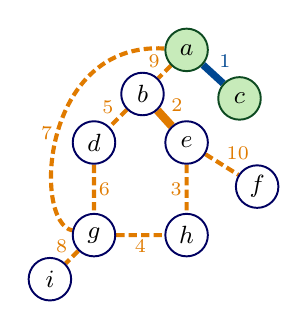
\begin{tikzpicture}[scale=0.56,every node/.append style={font=\footnotesize}]
  \node[gv,comp1] (a) at (3.1,5.2) {$a$};
  \node[gv] (b) at (2.1,4.2) {$b$};
  \node[gv,comp1] (c) at (4.3,4.1) {$c$};
  \node[gv] (d) at (1.0,3.1) {$d$};
  \node[gv] (e) at (3.1,3.1) {$e$};
  \node[gv] (f) at (4.7,2.1) {$f$};
  \node[gv] (g) at (1.0,1.0) {$g$};
  \node[gv] (h) at (3.1,1.0) {$h$};
  \node[gv] (i) at (0.0,0.0) {$i$};
  \begin{scope}[on background layer]
  \draw[mst] (a) -- node[gw,above right]{1} (c);
  \draw[nyss] (b) -- node[gw,above right]{2} (e);
  \draw[cand] (e) -- node[gw,left]{3} (h);
  \draw[cand] (g) -- node[gw,below]{4} (h);
  \draw[cand] (b) -- node[gw,above left]{5} (d);
  \draw[cand] (d) -- node[gw,right]{6} (g);
  \draw[cand] (a) .. controls (-0.2,5.4) and (-0.4,1.3) .. node[gw,left,pos=0.5]{7} (g);
  \draw[cand] (g) -- node[gw,above left]{8} (i);
  \draw[cand] (a) -- node[gw,above left]{9} (b);
  \draw[cand] (e) -- node[gw,above right]{10} (f);
  \end{scope}
\end{tikzpicture}\par
\footnotesize Kandidater: \emph{alla} kanter som återstår i listan.\\
Väljer \textbf{2} ($b$--$e$) — långt bort. Krusk\textbf{AL}: glob\textbf{AL}.
\end{column}
\begin{column}{0.49\textwidth}
\centering
{\small\bfseries\color{kthblue}Prim efter första kanten}\par\smallskip
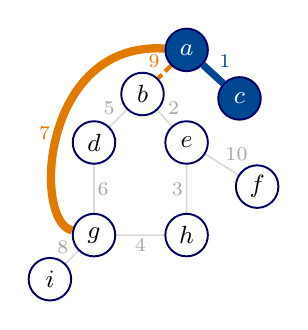
\begin{tikzpicture}[scale=0.56,every node/.append style={font=\footnotesize}]
  \node[gv,intree] (a) at (3.1,5.2) {$a$};
  \node[gv] (b) at (2.1,4.2) {$b$};
  \node[gv,intree] (c) at (4.3,4.1) {$c$};
  \node[gv] (d) at (1.0,3.1) {$d$};
  \node[gv] (e) at (3.1,3.1) {$e$};
  \node[gv] (f) at (4.7,2.1) {$f$};
  \node[gv] (g) at (1.0,1.0) {$g$};
  \node[gv] (h) at (3.1,1.0) {$h$};
  \node[gv] (i) at (0.0,0.0) {$i$};
  \begin{scope}[on background layer]
  \draw[mst] (a) -- node[gw,above right]{1} (c);
  \draw[faint] (b) -- node[gw,above right]{2} (e);
  \draw[faint] (e) -- node[gw,left]{3} (h);
  \draw[faint] (g) -- node[gw,below]{4} (h);
  \draw[faint] (b) -- node[gw,above left]{5} (d);
  \draw[faint] (d) -- node[gw,right]{6} (g);
  \draw[nyss] (a) .. controls (-0.2,5.4) and (-0.4,1.3) .. node[gw,left,pos=0.5]{7} (g);
  \draw[faint] (g) -- node[gw,above left]{8} (i);
  \draw[cand] (a) -- node[gw,above left]{9} (b);
  \draw[faint] (e) -- node[gw,above right]{10} (f);
  \end{scope}
\end{tikzpicture}\par
\footnotesize Kandidater: bara kanter \emph{ut ur trädet} $\{a,c\}$: 7 och 9.\\
Väljer \textbf{7} ($a$--$g$), trots att 2 finns. Prim: lokal.
\end{column}
\end{columns}
\varstrip{Kontrast}{grafen och första steget}{algoritmen}{vilken mängd ”billigast” gäller}
\end{frame}

% ---- gen/prim.tex ----
\begin{frame}{Prim på uppgiftens graf (rot $a$)}
\begin{columns}[T]
\begin{column}{0.47\textwidth}
\centering
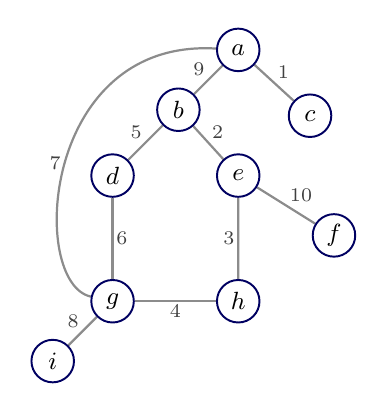
\begin{tikzpicture}[scale=0.76]
  \node[gv,onslide=<1>{draw=kthorange,line width=1.1pt},onslide=<2->{intree}] (a) at (3.1,5.2) {$a$};
  \node[gv,onslide=<2-6>{draw=kthorange,line width=1.1pt},onslide=<7->{intree}] (b) at (2.1,4.2) {$b$};
  \node[gv,onslide=<2>{draw=kthorange,line width=1.1pt},onslide=<3->{intree}] (c) at (4.3,4.1) {$c$};
  \node[gv,onslide=<4-7>{draw=kthorange,line width=1.1pt},onslide=<8->{intree}] (d) at (1.0,3.1) {$d$};
  \node[gv,onslide=<5>{draw=kthorange,line width=1.1pt},onslide=<6->{intree}] (e) at (3.1,3.1) {$e$};
  \node[gv,onslide=<6-9>{draw=kthorange,line width=1.1pt},onslide=<10->{intree}] (f) at (4.7,2.1) {$f$};
  \node[gv,onslide=<2-3>{draw=kthorange,line width=1.1pt},onslide=<4->{intree}] (g) at (1.0,1.0) {$g$};
  \node[gv,onslide=<4>{draw=kthorange,line width=1.1pt},onslide=<5->{intree}] (h) at (3.1,1.0) {$h$};
  \node[gv,onslide=<4-8>{draw=kthorange,line width=1.1pt},onslide=<9->{intree}] (i) at (0.0,0.0) {$i$};
  \begin{scope}[on background layer]
  \draw[ge,onslide=<2>{cand},onslide=<3>{nyss},onslide=<4->{mst}] (a) -- node[gw,above right]{1} (c);
  \draw[ge,onslide=<6>{cand},onslide=<7>{nyss},onslide=<8->{mst}] (b) -- node[gw,above right]{2} (e);
  \draw[ge,onslide=<5>{cand},onslide=<6>{nyss},onslide=<7->{mst}] (e) -- node[gw,left]{3} (h);
  \draw[ge,onslide=<4>{cand},onslide=<5>{nyss},onslide=<6->{mst}] (g) -- node[gw,below]{4} (h);
  \draw[ge,onslide=<7>{cand},onslide=<8>{nyss},onslide=<9->{mst}] (b) -- node[gw,above left]{5} (d);
  \draw[ge,onslide=<4-6>{cand},onslide=<7->{faint}] (d) -- node[gw,right]{6} (g);
  \draw[ge,onslide=<2-3>{cand},onslide=<4>{nyss},onslide=<5->{mst}] (a) .. controls (-0.2,5.4) and (-0.4,1.3) .. node[gw,left,pos=0.5]{7} (g);
  \draw[ge,onslide=<4-8>{cand},onslide=<9>{nyss},onslide=<10->{mst}] (g) -- node[gw,above left]{8} (i);
  \draw[ge,onslide=<2-5>{cand},onslide=<6->{faint}] (a) -- node[gw,above left]{9} (b);
  \draw[ge,onslide=<6-9>{cand},onslide=<10->{nyss}] (e) -- node[gw,above right]{10} (f);
  \end{scope}
\end{tikzpicture}
\end{column}
\begin{column}{0.5\textwidth}
{\footnotesize\bfseries\color{kthnavy}Prioritetskö $Q$ (nyckel = billigaste kant in i trädet)}\par\smallskip
\footnotesize
\only<1>{%
\begin{tabular}{@{}l@{\quad}r@{\quad}l@{}}
\toprule hörn & key & $\pi$\\\midrule
$a$ & $0$ & --\\
\multicolumn{3}{@{}l}{\color{black!50}+ 8 hörn med nyckel $\infty$}\\
\bottomrule
\end{tabular}\par\smallskip
{\scriptsize\color{kthblue}Utplockade: --}}
\only<2>{%
\begin{tabular}{@{}l@{\quad}r@{\quad}l@{}}
\toprule hörn & key & $\pi$\\\midrule
$c$ & $1$ & $a$\ \textcolor{kthgrass}{(ny)}\\
$g$ & $7$ & $a$\ \textcolor{kthgrass}{(ny)}\\
$b$ & $9$ & $a$\ \textcolor{kthgrass}{(ny)}\\
\multicolumn{3}{@{}l}{\color{black!50}+ 5 hörn med nyckel $\infty$}\\
\bottomrule
\end{tabular}\par\smallskip
{\scriptsize\color{kthblue}Utplockade: $a$}}
\only<3>{%
\begin{tabular}{@{}l@{\quad}r@{\quad}l@{}}
\toprule hörn & key & $\pi$\\\midrule
$g$ & $7$ & $a$\\
$b$ & $9$ & $a$\\
\multicolumn{3}{@{}l}{\color{black!50}+ 5 hörn med nyckel $\infty$}\\
\bottomrule
\end{tabular}\par\smallskip
{\scriptsize\color{kthblue}Utplockade: $a$, $c$}}
\only<4>{%
\begin{tabular}{@{}l@{\quad}r@{\quad}l@{}}
\toprule hörn & key & $\pi$\\\midrule
$h$ & $4$ & $g$\ \textcolor{kthgrass}{(ny)}\\
$d$ & $6$ & $g$\ \textcolor{kthgrass}{(ny)}\\
$i$ & $8$ & $g$\ \textcolor{kthgrass}{(ny)}\\
$b$ & $9$ & $a$\\
\multicolumn{3}{@{}l}{\color{black!50}+ 2 hörn med nyckel $\infty$}\\
\bottomrule
\end{tabular}\par\smallskip
{\scriptsize\color{kthblue}Utplockade: $a$, $c$, $g$}}
\only<5>{%
\begin{tabular}{@{}l@{\quad}r@{\quad}l@{}}
\toprule hörn & key & $\pi$\\\midrule
$e$ & $3$ & $h$\ \textcolor{kthgrass}{(ny)}\\
$d$ & $6$ & $g$\\
$i$ & $8$ & $g$\\
$b$ & $9$ & $a$\\
\multicolumn{3}{@{}l}{\color{black!50}+ 1 hörn med nyckel $\infty$}\\
\bottomrule
\end{tabular}\par\smallskip
{\scriptsize\color{kthblue}Utplockade: $a$, $c$, $g$, $h$}}
\only<6>{%
\begin{tabular}{@{}l@{\quad}r@{\quad}l@{}}
\toprule hörn & key & $\pi$\\\midrule
$b$ & $2$ & $e$\ \textcolor{brick}{(var 9)}\\
$d$ & $6$ & $g$\\
$i$ & $8$ & $g$\\
$f$ & $10$ & $e$\ \textcolor{kthgrass}{(ny)}\\

\bottomrule
\end{tabular}\par\smallskip
{\scriptsize\color{kthblue}Utplockade: $a$, $c$, $g$, $h$, $e$}}
\only<7>{%
\begin{tabular}{@{}l@{\quad}r@{\quad}l@{}}
\toprule hörn & key & $\pi$\\\midrule
$d$ & $5$ & $b$\ \textcolor{brick}{(var 6)}\\
$i$ & $8$ & $g$\\
$f$ & $10$ & $e$\\

\bottomrule
\end{tabular}\par\smallskip
{\scriptsize\color{kthblue}Utplockade: $a$, $c$, $g$, $h$, $e$, $b$}}
\only<8>{%
\begin{tabular}{@{}l@{\quad}r@{\quad}l@{}}
\toprule hörn & key & $\pi$\\\midrule
$i$ & $8$ & $g$\\
$f$ & $10$ & $e$\\

\bottomrule
\end{tabular}\par\smallskip
{\scriptsize\color{kthblue}Utplockade: $a$, $c$, $g$, $h$, $e$, $b$, $d$}}
\only<9>{%
\begin{tabular}{@{}l@{\quad}r@{\quad}l@{}}
\toprule hörn & key & $\pi$\\\midrule
$f$ & $10$ & $e$\\

\bottomrule
\end{tabular}\par\smallskip
{\scriptsize\color{kthblue}Utplockade: $a$, $c$, $g$, $h$, $e$, $b$, $d$, $i$}}
\only<10>{%
\begin{tabular}{@{}l@{\quad}r@{\quad}l@{}}
\toprule hörn & key & $\pi$\\\midrule
\multicolumn{3}{@{}l}{\color{black!50}(tom)}\\

\bottomrule
\end{tabular}\par\smallskip
{\scriptsize\color{kthblue}Utplockade: $a$, $c$, $g$, $h$, $e$, $b$, $d$, $i$, $f$}}
\end{column}
\end{columns}
\vfill
\begin{tcolorbox}[enhanced,colback=kthlight!50,colframe=kthsky,boxrule=0.4pt,arc=2pt,
  left=4pt,right=4pt,top=1pt,bottom=1pt,fontupper=\small,height=0.95cm,valign=center]
\only<1>{Starta i $a$: $\mathit{key}[a]=0$, alla andra $\infty$. Alla hörn ligger i kön.}\only<2>{Plocka ut $a$. Grannarna får nycklar: $c$ (1), $g$ (7), $b$ (9).}\only<3>{Plocka ut $c$ (1). Inga nya grannar. Kön är lokal: bara kanter \emph{ut ur trädet} räknas.}\only<4>{Plocka ut $g$ (7). Nya nycklar: $h$ (4), $d$ (6), $i$ (8).}\only<5>{Plocka ut $h$ (4). Ny nyckel: $e$ (3).}\only<6>{Plocka ut $e$ (3). \textsc{Decrease-Key}: $b$ går från 9 till 2. Ny: $f$ (10).}\only<7>{Plocka ut $b$ (2). \textsc{Decrease-Key}: $d$ går från 6 till 5.}\only<8>{Plocka ut $d$ (5). Kanten $d$--$g$ (6) blev aldrig trädkant.}\only<9>{Plocka ut $i$ (8).}\only<10>{Plocka ut $f$ (10). Vikt $1+7+4+3+2+5+8+10=40$. Samma träd som Kruskal (unika vikter!).}
\end{tcolorbox}
\end{frame}


\begin{frame}{Facit och kontroll}
\begin{columns}[T]
\begin{column}{0.44\textwidth}
\centering
% ---- gen/graf-mst.tex ----
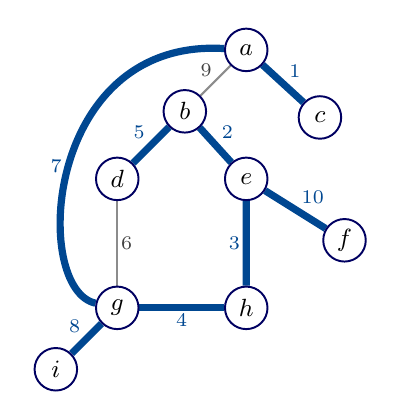
\begin{tikzpicture}[scale=0.78]
  \node[gv] (a) at (3.1,5.2) {$a$};
  \node[gv] (b) at (2.1,4.2) {$b$};
  \node[gv] (c) at (4.3,4.1) {$c$};
  \node[gv] (d) at (1.0,3.1) {$d$};
  \node[gv] (e) at (3.1,3.1) {$e$};
  \node[gv] (f) at (4.7,2.1) {$f$};
  \node[gv] (g) at (1.0,1.0) {$g$};
  \node[gv] (h) at (3.1,1.0) {$h$};
  \node[gv] (i) at (0.0,0.0) {$i$};
  \begin{scope}[on background layer]
  \draw[mst] (a) -- node[gw,above right]{1} (c);
  \draw[mst] (b) -- node[gw,above right]{2} (e);
  \draw[mst] (e) -- node[gw,left]{3} (h);
  \draw[mst] (g) -- node[gw,below]{4} (h);
  \draw[mst] (b) -- node[gw,above left]{5} (d);
  \draw[ge] (d) -- node[gw,right]{6} (g);
  \draw[mst] (a) .. controls (-0.2,5.4) and (-0.4,1.3) .. node[gw,left,pos=0.5]{7} (g);
  \draw[mst] (g) -- node[gw,above left]{8} (i);
  \draw[ge] (a) -- node[gw,above left]{9} (b);
  \draw[mst] (e) -- node[gw,above right]{10} (f);
  \end{scope}
\end{tikzpicture}

\end{column}
\begin{column}{0.53\textwidth}
\small
\begin{itemize}\setlength{\itemsep}{3pt}
  \item Kanter: $1,2,3,4,5,7,8,10$. \quad Vikt: $\mathbf{40}$.
  \item Kruskal förkastar \textbf{6} och \textbf{9}: båda sluter cykler.
  \item Prim från $a$ plockar i ordningen $a,c,g,h,e,b,d,i,f$.
  \item Samma träd, olika \emph{ordning}. Det är ingen slump: med unika vikter
        finns bara ett MST.
\end{itemize}
\begin{ahabox}
\textbf{Kontroll som alltid fungerar:} rätt antal kanter ($|V|-1$), ingen cykel,
och varje förkastad kant är den tyngsta på sin cykel.
\end{ahabox}
\end{column}
\end{columns}
\end{frame}

% ---------------------------------------------------------------- kaninhål
{\kaninbg
\begin{frame}{\kh Varför fungerar girigheten? Snitt och cykler}
\begin{columns}[T]
\begin{column}{0.49\textwidth}
\centering
{\small\bfseries\color{plum}Snittegenskapen}\par
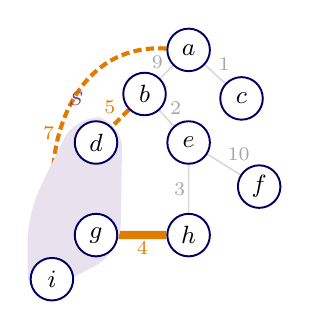
\begin{tikzpicture}[scale=0.56,every node/.append style={font=\footnotesize}]
  \node[gv] (a) at (3.1,5.2) {$a$};
  \node[gv] (b) at (2.1,4.2) {$b$};
  \node[gv] (c) at (4.3,4.1) {$c$};
  \node[gv] (d) at (1.0,3.1) {$d$};
  \node[gv] (e) at (3.1,3.1) {$e$};
  \node[gv] (f) at (4.7,2.1) {$f$};
  \node[gv] (g) at (1.0,1.0) {$g$};
  \node[gv] (h) at (3.1,1.0) {$h$};
  \node[gv] (i) at (0.0,0.0) {$i$};
  \begin{scope}[on background layer]
  \draw[faint] (a) -- node[gw,above right]{1} (c);
  \draw[faint] (b) -- node[gw,above right]{2} (e);
  \draw[faint] (e) -- node[gw,left]{3} (h);
  \draw[nyss] (g) -- node[gw,below]{4} (h);
  \draw[cand] (b) -- node[gw,above left]{5} (d);
  \draw[ge] (d) -- node[gw,right]{6} (g);
  \draw[cand] (a) .. controls (-0.2,5.4) and (-0.4,1.3) .. node[gw,left,pos=0.5]{7} (g);
  \draw[ge] (g) -- node[gw,above left]{8} (i);
  \draw[faint] (a) -- node[gw,above left]{9} (b);
  \draw[faint] (e) -- node[gw,above right]{10} (f);
  \end{scope}
  \begin{scope}[on background layer]
  \fill[plum!15,rounded corners=10pt] (-0.55,-0.5) -- (1.55,0.6) -- (1.6,3.6) -- (0.55,3.75) -- (-0.55,1.5) -- cycle;
  \end{scope}
  \node[font=\scriptsize\bfseries,text=plum] at (0.55,4.1) {$S$};
\end{tikzpicture}\par
\footnotesize Kanterna över snittet $S=\{d,g,i\}$: 4, 5, 7.
Den lättaste, \textbf{4}, ingår i \emph{varje} MST.
\end{column}
\begin{column}{0.49\textwidth}
\centering
{\small\bfseries\color{kthgreen}Cykelegenskapen}\par
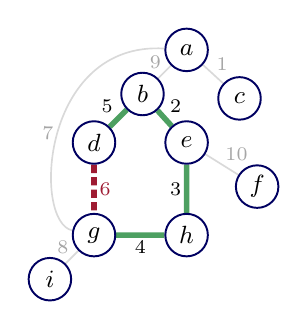
\begin{tikzpicture}[scale=0.56,every node/.append style={font=\footnotesize}]
  \node[gv] (a) at (3.1,5.2) {$a$};
  \node[gv] (b) at (2.1,4.2) {$b$};
  \node[gv] (c) at (4.3,4.1) {$c$};
  \node[gv] (d) at (1.0,3.1) {$d$};
  \node[gv] (e) at (3.1,3.1) {$e$};
  \node[gv] (f) at (4.7,2.1) {$f$};
  \node[gv] (g) at (1.0,1.0) {$g$};
  \node[gv] (h) at (3.1,1.0) {$h$};
  \node[gv] (i) at (0.0,0.0) {$i$};
  \begin{scope}[on background layer]
  \draw[faint] (a) -- node[gw,above right]{1} (c);
  \draw[draw=kthgrass,line width=2pt] (b) -- node[gw,above right]{2} (e);
  \draw[draw=kthgrass,line width=2pt] (e) -- node[gw,left]{3} (h);
  \draw[draw=kthgrass,line width=2pt] (g) -- node[gw,below]{4} (h);
  \draw[draw=kthgrass,line width=2pt] (b) -- node[gw,above left]{5} (d);
  \draw[rejnu] (d) -- node[gw,right]{6} (g);
  \draw[faint] (a) .. controls (-0.2,5.4) and (-0.4,1.3) .. node[gw,left,pos=0.5]{7} (g);
  \draw[faint] (g) -- node[gw,above left]{8} (i);
  \draw[faint] (a) -- node[gw,above left]{9} (b);
  \draw[faint] (e) -- node[gw,above right]{10} (f);
  \end{scope}
\end{tikzpicture}\par
\footnotesize På cykeln $b$--$d$--$g$--$h$--$e$ är \textbf{6} tyngst.
Den ingår i \emph{inget} MST.
\end{column}
\end{columns}
\vfill
\begin{kaninbox}[fontupper=\footnotesize]
\textbf{Kruskal:} kanten den tar är lättast över snittet (sin komponent, resten).
\textbf{Prim:} kanten den tar är lättast över snittet (trädet, resten).
Samma sats, två olika snitt. Därför är båda korrekta.
\end{kaninbox}
\end{frame}}

{\kaninbg
\begin{frame}{\kh Union--Find: hur Kruskal vet vad som hänger ihop}
\begin{columns}[T]
\begin{column}{0.52\textwidth}
\small
\begin{itemize}\setlength{\itemsep}{2pt}
  \item Varje komponent är ett träd av föräldrapekare; roten är komponentens namn.
  \item \textsc{Find}$(x)$: följ pekarna till roten.
  \item \textsc{Union}: häng den \emph{mindre} roten under den större.
  \item \textbf{Stigkomprimering:} låt alla på vägen peka direkt på roten.
  \item Båda knepen: amorterat $O(\alpha(n))$ per operation. $\alpha$ är i praktiken $\le4$.
\end{itemize}
\end{column}
\begin{column}{0.45\textwidth}
\centering
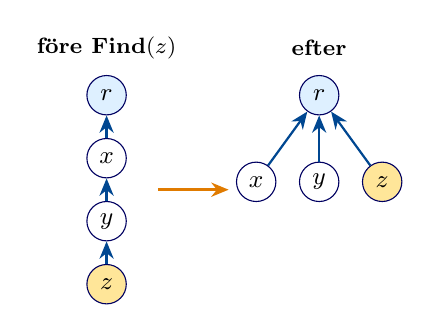
\begin{tikzpicture}[font=\small,
   uf/.style={circle,draw=kthnavy,minimum size=5mm,inner sep=0pt},
   p/.style={->,draw=kthblue,line width=0.8pt}]
  \node[font=\footnotesize\bfseries] at (0.7,3.3) {före \textsc{Find}$(z)$};
  \node[uf,fill=kthlight] (r) at (0.7,2.7) {$r$};
  \node[uf,fill=white] (x) at (0.7,1.9) {$x$};
  \node[uf,fill=white] (y) at (0.7,1.1) {$y$};
  \node[uf,fill=lampyellow!50] (z) at (0.7,0.3) {$z$};
  \draw[p] (x) -- (r); \draw[p] (y) -- (x); \draw[p] (z) -- (y);
  \draw[->,kthorange,line width=1pt] (1.35,1.5) -- (2.25,1.5);
  \node[font=\footnotesize\bfseries] at (3.4,3.3) {efter};
  \node[uf,fill=kthlight] (r2) at (3.4,2.7) {$r$};
  \node[uf,fill=white] (x2) at (2.6,1.6) {$x$};
  \node[uf,fill=white] (y2) at (3.4,1.6) {$y$};
  \node[uf,fill=lampyellow!50] (z2) at (4.2,1.6) {$z$};
  \draw[p] (x2) -- (r2); \draw[p] (y2) -- (r2); \draw[p] (z2) -- (r2);
\end{tikzpicture}
\end{column}
\end{columns}
\vfill
\begin{kaninbox}[fontupper=\footnotesize]
\textbf{Kruskals tid:} sortering $O(|E|\log|E|)$ + $|E|$ \textsc{Find} och $|V|-1$
\textsc{Union}. Sorteringen dominerar. Och $\log|E|\le\log|V|^2=2\log|V|$, så
$O(|E|\log|E|)=O(|E|\log|V|)$.
\end{kaninbox}
\end{frame}}

{\kaninbg
\begin{frame}{\kh Prims tid beror på prioritetskön}
\centering
\small
\begin{tabular}{@{}llll@{}}
\toprule
Kö & \textsc{ExtractMin} & \textsc{DecreaseKey} & Totalt\\
\midrule
osorterad array & $O(|V|)$ & $O(1)$ & $O(|V|^2)$\\
binär heap & $O(\log|V|)$ & $O(\log|V|)$ & $O(|E|\log|V|)$\\
Fibonacciheap & $O(\log|V|)$ am. & $O(1)$ am. & $O(|E|+|V|\log|V|)$\\
”lat” heap med kanter & $O(\log|E|)$ & — (lägg in dubbletter) & $O(|E|\log|V|)$\\
\bottomrule
\end{tabular}
\vfill
\begin{columns}[T]
\begin{column}{0.49\textwidth}
\begin{kaninbox}[fontupper=\footnotesize]
\textbf{Tät graf}, $|E|=\Theta(|V|^2)$: arrayen vinner. $O(|V|^2)$ är dessutom
\emph{linjärt i grannmatrisens storlek}.
\end{kaninbox}
\end{column}
\begin{column}{0.49\textwidth}
\begin{kaninbox}[fontupper=\footnotesize]
\textbf{Gles graf}, $|E|=O(|V|)$: heapen vinner, $O(|V|\log|V|)$.
Samma algoritm, olika datastruktur, olika ”bästa”.
\end{kaninbox}
\end{column}
\end{columns}
\varstrip{Separation}{algoritmen (Prim)}{datastrukturen och tätheten}{att komplexitet hör till algoritm \emph{plus} datastruktur}
\end{frame}}

{\kaninbg
\begin{frame}{\kh Borůvka (1926): alla komponenter väljer samtidigt}
\begin{columns}[T]
\begin{column}{0.49\textwidth}
\centering
{\small\bfseries\color{kthblue}Runda 1}\par
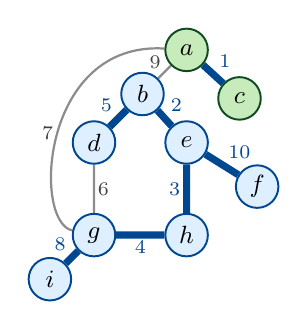
\begin{tikzpicture}[scale=0.56,every node/.append style={font=\footnotesize}]
  \node[gv,comp1] (a) at (3.1,5.2) {$a$};
  \node[gv,comp2] (b) at (2.1,4.2) {$b$};
  \node[gv,comp1] (c) at (4.3,4.1) {$c$};
  \node[gv,comp2] (d) at (1.0,3.1) {$d$};
  \node[gv,comp2] (e) at (3.1,3.1) {$e$};
  \node[gv,comp2] (f) at (4.7,2.1) {$f$};
  \node[gv,comp2] (g) at (1.0,1.0) {$g$};
  \node[gv,comp2] (h) at (3.1,1.0) {$h$};
  \node[gv,comp2] (i) at (0.0,0.0) {$i$};
  \begin{scope}[on background layer]
  \draw[mst] (a) -- node[gw,above right]{1} (c);
  \draw[mst] (b) -- node[gw,above right]{2} (e);
  \draw[mst] (e) -- node[gw,left]{3} (h);
  \draw[mst] (g) -- node[gw,below]{4} (h);
  \draw[mst] (b) -- node[gw,above left]{5} (d);
  \draw[ge] (d) -- node[gw,right]{6} (g);
  \draw[ge] (a) .. controls (-0.2,5.4) and (-0.4,1.3) .. node[gw,left,pos=0.5]{7} (g);
  \draw[mst] (g) -- node[gw,above left]{8} (i);
  \draw[ge] (a) -- node[gw,above left]{9} (b);
  \draw[mst] (e) -- node[gw,above right]{10} (f);
  \end{scope}
\end{tikzpicture}\par
\footnotesize Varje hörn tar sin billigaste kant:\\ 1, 2, 3, 4, 5, 8, 10. Två komponenter kvar.
\end{column}
\begin{column}{0.49\textwidth}
\centering
{\small\bfseries\color{kthblue}Runda 2}\par
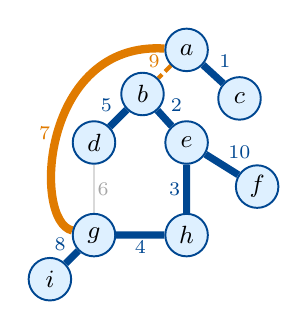
\begin{tikzpicture}[scale=0.56,every node/.append style={font=\footnotesize}]
  \node[gv,comp2] (a) at (3.1,5.2) {$a$};
  \node[gv,comp2] (b) at (2.1,4.2) {$b$};
  \node[gv,comp2] (c) at (4.3,4.1) {$c$};
  \node[gv,comp2] (d) at (1.0,3.1) {$d$};
  \node[gv,comp2] (e) at (3.1,3.1) {$e$};
  \node[gv,comp2] (f) at (4.7,2.1) {$f$};
  \node[gv,comp2] (g) at (1.0,1.0) {$g$};
  \node[gv,comp2] (h) at (3.1,1.0) {$h$};
  \node[gv,comp2] (i) at (0.0,0.0) {$i$};
  \begin{scope}[on background layer]
  \draw[mst] (a) -- node[gw,above right]{1} (c);
  \draw[mst] (b) -- node[gw,above right]{2} (e);
  \draw[mst] (e) -- node[gw,left]{3} (h);
  \draw[mst] (g) -- node[gw,below]{4} (h);
  \draw[mst] (b) -- node[gw,above left]{5} (d);
  \draw[faint] (d) -- node[gw,right]{6} (g);
  \draw[nyss] (a) .. controls (-0.2,5.4) and (-0.4,1.3) .. node[gw,left,pos=0.5]{7} (g);
  \draw[mst] (g) -- node[gw,above left]{8} (i);
  \draw[cand] (a) -- node[gw,above left]{9} (b);
  \draw[mst] (e) -- node[gw,above right]{10} (f);
  \end{scope}
\end{tikzpicture}\par
\footnotesize Billigaste kanten mellan dem: \textbf{7} (inte 9). Klart.
\end{column}
\end{columns}
\vfill
\begin{kaninbox}[fontupper=\footnotesize]
Antalet komponenter minst halveras per runda $\Rightarrow$ $O(\log|V|)$ rundor à $O(|E|)$:
$O(|E|\log|V|)$. Äldst av de tre, och lättast att parallellisera. (Kräver unika vikter
eller konsekvent tie-break — annars kan två komponenter välja varsin kant och bilda en cykel.)
\end{kaninbox}
\end{frame}}

% ---------------------------------------------------------------- variation
\begin{frame}{Vanligt fel: ”billigaste kanten från där jag står”}
\begin{columns}[T]
\begin{column}{0.42\textwidth}
\centering
% ---- gen/girig.tex ----
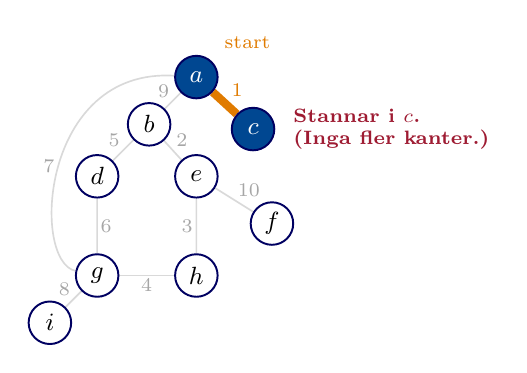
\begin{tikzpicture}[scale=0.6,every node/.append style={font=\footnotesize}]
  \node[gv,intree] (a) at (3.1,5.2) {$a$};
  \node[gv] (b) at (2.1,4.2) {$b$};
  \node[gv,intree] (c) at (4.3,4.1) {$c$};
  \node[gv] (d) at (1.0,3.1) {$d$};
  \node[gv] (e) at (3.1,3.1) {$e$};
  \node[gv] (f) at (4.7,2.1) {$f$};
  \node[gv] (g) at (1.0,1.0) {$g$};
  \node[gv] (h) at (3.1,1.0) {$h$};
  \node[gv] (i) at (0.0,0.0) {$i$};
  \begin{scope}[on background layer]
  \draw[nyss] (a) -- node[gw,above right]{1} (c);
  \draw[faint] (b) -- node[gw,above right]{2} (e);
  \draw[faint] (e) -- node[gw,left]{3} (h);
  \draw[faint] (g) -- node[gw,below]{4} (h);
  \draw[faint] (b) -- node[gw,above left]{5} (d);
  \draw[faint] (d) -- node[gw,right]{6} (g);
  \draw[faint] (a) .. controls (-0.2,5.4) and (-0.4,1.3) .. node[gw,left,pos=0.5]{7} (g);
  \draw[faint] (g) -- node[gw,above left]{8} (i);
  \draw[faint] (a) -- node[gw,above left]{9} (b);
  \draw[faint] (e) -- node[gw,above right]{10} (f);
  \end{scope}
  \node[font=\scriptsize\bfseries,text=brick,right=3pt of c,align=left] {Stannar i $c$.\\(Inga fler kanter.)};
  \node[font=\scriptsize,text=kthorange,above right=1pt and 1pt of a] {start};
\end{tikzpicture}

\end{column}
\begin{column}{0.55\textwidth}
\begin{missbox}
”Prim = gå längs billigaste kanten från det senaste hörnet.”
\end{missbox}
\small
Från $a$: billigast är 1 till $c$. Kommer till $c$. Stannar i $c$.
\medskip

Det där är en \emph{promenad}, inte Prim. Prim tittar på alla kanter
ut ur \emph{hela trädet} $\{a,c\}$, inte bara ut ur $c$.
\medskip

Och även när promenaden inte kör fast blir den en stig — ett spännande träd behöver
kunna förgrena sig.
\end{column}
\end{columns}
\varstrip{Kontrast}{grafen, startpunkten}{”ut ur senaste hörnet” / ”ut ur trädet”}{snittet går runt hela trädet}
\end{frame}

\begin{frame}{Prim är inte Dijkstra}
\begin{columns}[T]
\begin{column}{0.33\textwidth}
\centering
{\small\bfseries\color{kthblue}MST (Prim), vikt 40}\par
% ---- gen/kontrast-mst.tex ----
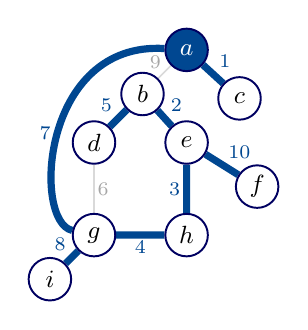
\begin{tikzpicture}[scale=0.56,every node/.append style={font=\footnotesize}]
  \node[gv,intree] (a) at (3.1,5.2) {$a$};
  \node[gv] (b) at (2.1,4.2) {$b$};
  \node[gv] (c) at (4.3,4.1) {$c$};
  \node[gv] (d) at (1.0,3.1) {$d$};
  \node[gv] (e) at (3.1,3.1) {$e$};
  \node[gv] (f) at (4.7,2.1) {$f$};
  \node[gv] (g) at (1.0,1.0) {$g$};
  \node[gv] (h) at (3.1,1.0) {$h$};
  \node[gv] (i) at (0.0,0.0) {$i$};
  \begin{scope}[on background layer]
  \draw[mst] (a) -- node[gw,above right]{1} (c);
  \draw[mst] (b) -- node[gw,above right]{2} (e);
  \draw[mst] (e) -- node[gw,left]{3} (h);
  \draw[mst] (g) -- node[gw,below]{4} (h);
  \draw[mst] (b) -- node[gw,above left]{5} (d);
  \draw[faint] (d) -- node[gw,right]{6} (g);
  \draw[mst] (a) .. controls (-0.2,5.4) and (-0.4,1.3) .. node[gw,left,pos=0.5]{7} (g);
  \draw[mst] (g) -- node[gw,above left]{8} (i);
  \draw[faint] (a) -- node[gw,above left]{9} (b);
  \draw[mst] (e) -- node[gw,above right]{10} (f);
  \end{scope}
\end{tikzpicture}

\end{column}
\begin{column}{0.33\textwidth}
\centering
{\small\bfseries\color{plum}Kortaste-vägträd från $a$, vikt 47}\par
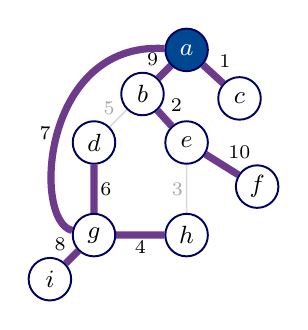
\begin{tikzpicture}[scale=0.56,every node/.append style={font=\footnotesize}]
  \node[gv,intree] (a) at (3.1,5.2) {$a$};
  \node[gv] (b) at (2.1,4.2) {$b$};
  \node[gv] (c) at (4.3,4.1) {$c$};
  \node[gv] (d) at (1.0,3.1) {$d$};
  \node[gv] (e) at (3.1,3.1) {$e$};
  \node[gv] (f) at (4.7,2.1) {$f$};
  \node[gv] (g) at (1.0,1.0) {$g$};
  \node[gv] (h) at (3.1,1.0) {$h$};
  \node[gv] (i) at (0.0,0.0) {$i$};
  \begin{scope}[on background layer]
  \draw[draw=plum,line width=2.6pt] (a) -- node[gw,above right]{1} (c);
  \draw[draw=plum,line width=2.6pt] (b) -- node[gw,above right]{2} (e);
  \draw[faint] (e) -- node[gw,left]{3} (h);
  \draw[draw=plum,line width=2.6pt] (g) -- node[gw,below]{4} (h);
  \draw[faint] (b) -- node[gw,above left]{5} (d);
  \draw[draw=plum,line width=2.6pt] (d) -- node[gw,right]{6} (g);
  \draw[draw=plum,line width=2.6pt] (a) .. controls (-0.2,5.4) and (-0.4,1.3) .. node[gw,left,pos=0.5]{7} (g);
  \draw[draw=plum,line width=2.6pt] (g) -- node[gw,above left]{8} (i);
  \draw[draw=plum,line width=2.6pt] (a) -- node[gw,above left]{9} (b);
  \draw[draw=plum,line width=2.6pt] (e) -- node[gw,above right]{10} (f);
  \end{scope}
\end{tikzpicture}\par
{\scriptsize\color{plum}avstånd: $b$ 9, $c$ 1, $d$ 13, $e$ 11, $f$ 21, $g$ 7, $h$ 11, $i$ 15}
\end{column}
\begin{column}{0.3\textwidth}
\footnotesize
Samma skelett: kö, \textsc{ExtractMin}, \textsc{DecreaseKey}. En rad skiljer:\par\smallskip
Prim: $\mathit{key}[v]\gets w(u,v)$\par
Dijkstra: $d[v]\gets d[u]+w(u,v)$\par\smallskip
I MST är vägen $a\leadsto b$ lång: $7+4+3+2=16$. Dijkstra tar kanten 9 direkt.
MST minimerar \emph{summan över trädet}, inte avståndet från $a$.
\end{column}
\end{columns}
\varstrip{Kontrast}{graf, rot, köstruktur}{nyckeln: kantvikt eller avstånd}{vad som minimeras}
\end{frame}

\begin{frame}{Vad beror MST på? Ändra vikterna}
\begin{columns}[T]
\begin{column}{0.68\textwidth}
\scriptsize
\renewcommand{\arraystretch}{1.3}
\begin{tabular}{@{}p{0.27\linewidth}p{0.13\linewidth}p{0.52\linewidth}@{}}
\toprule
\textbf{Ändring} & \textbf{MST} & \textbf{Kortaste-vägträd från $a$}\\
\midrule
$w\mapsto w^2$ & samma & \textbf{ändras}: $b$ nås nu via $e$ ($78<81$)\\
$w\mapsto w-5$ & samma & \textbf{odefinierat}: fram och tillbaka på en negativ kant\\
$w\mapsto w+c$ & samma & kan ändras: straffar stigar med många kanter\\
byt $5\leftrightarrow6$ på $b$--$d$, $d$--$g$ & \textbf{ändras} & samma (här)\\
\bottomrule
\end{tabular}
\medskip

\small
Varje \emph{strikt växande} funktion av vikterna ger samma MST.
Kruskal tittar ju bara på den sorterade ordningen.
\end{column}
\begin{column}{0.29\textwidth}
\centering
{\scriptsize\bfseries\color{plum}$w^2$: nytt kortaste-vägträd}\par
% ---- gen/sq-spt.tex ----
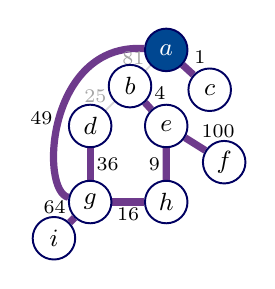
\begin{tikzpicture}[scale=0.46,every node/.append style={font=\footnotesize}]
  \node[gv,intree] (a) at (3.1,5.2) {$a$};
  \node[gv] (b) at (2.1,4.2) {$b$};
  \node[gv] (c) at (4.3,4.1) {$c$};
  \node[gv] (d) at (1.0,3.1) {$d$};
  \node[gv] (e) at (3.1,3.1) {$e$};
  \node[gv] (f) at (4.7,2.1) {$f$};
  \node[gv] (g) at (1.0,1.0) {$g$};
  \node[gv] (h) at (3.1,1.0) {$h$};
  \node[gv] (i) at (0.0,0.0) {$i$};
  \begin{scope}[on background layer]
  \draw[draw=plum,line width=2.6pt] (a) -- node[gw,above right]{1} (c);
  \draw[draw=plum,line width=2.6pt] (b) -- node[gw,above right]{4} (e);
  \draw[draw=plum,line width=2.6pt] (e) -- node[gw,left]{9} (h);
  \draw[draw=plum,line width=2.6pt] (g) -- node[gw,below]{16} (h);
  \draw[faint] (b) -- node[gw,above left]{25} (d);
  \draw[draw=plum,line width=2.6pt] (d) -- node[gw,right]{36} (g);
  \draw[draw=plum,line width=2.6pt] (a) .. controls (-0.2,5.4) and (-0.4,1.3) .. node[gw,left,pos=0.5]{49} (g);
  \draw[draw=plum,line width=2.6pt] (g) -- node[gw,above left]{64} (i);
  \draw[faint] (a) -- node[gw,above left]{81} (b);
  \draw[draw=plum,line width=2.6pt] (e) -- node[gw,above right]{100} (f);
  \end{scope}
\end{tikzpicture}

\end{column}
\end{columns}
\varstrip{Separation}{grafen}{vikterna}{MST beror på ordningen, kortaste väg på summorna}
\end{frame}

\begin{frame}{Är MST unikt?}
\begin{columns}[T]
\begin{column}{0.3\textwidth}
\centering
{\scriptsize\bfseries Om $d$--$g$ också väger 5 \dots}\par
% ---- gen/tie1.tex ----
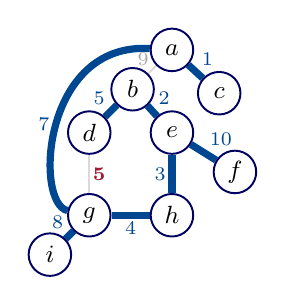
\begin{tikzpicture}[scale=0.5,every node/.append style={font=\footnotesize}]
  \node[gv] (a) at (3.1,5.2) {$a$};
  \node[gv] (b) at (2.1,4.2) {$b$};
  \node[gv] (c) at (4.3,4.1) {$c$};
  \node[gv] (d) at (1.0,3.1) {$d$};
  \node[gv] (e) at (3.1,3.1) {$e$};
  \node[gv] (f) at (4.7,2.1) {$f$};
  \node[gv] (g) at (1.0,1.0) {$g$};
  \node[gv] (h) at (3.1,1.0) {$h$};
  \node[gv] (i) at (0.0,0.0) {$i$};
  \begin{scope}[on background layer]
  \draw[mst] (a) -- node[gw,above right]{1} (c);
  \draw[mst] (b) -- node[gw,above right]{2} (e);
  \draw[mst] (e) -- node[gw,left]{3} (h);
  \draw[mst] (g) -- node[gw,below]{4} (h);
  \draw[mst] (b) -- node[gw,above left]{5} (d);
  \draw[faint] (d) -- node[gw,right]{\textbf{\textcolor{brick}{5}}} (g);
  \draw[mst] (a) .. controls (-0.2,5.4) and (-0.4,1.3) .. node[gw,left,pos=0.5]{7} (g);
  \draw[mst] (g) -- node[gw,above left]{8} (i);
  \draw[faint] (a) -- node[gw,above left]{9} (b);
  \draw[mst] (e) -- node[gw,above right]{10} (f);
  \end{scope}
\end{tikzpicture}

\end{column}
\begin{column}{0.3\textwidth}
\centering
{\scriptsize\bfseries \dots\ finns två MST, båda 40}\par
% ---- gen/tie2.tex ----
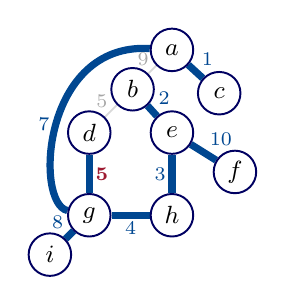
\begin{tikzpicture}[scale=0.5,every node/.append style={font=\footnotesize}]
  \node[gv] (a) at (3.1,5.2) {$a$};
  \node[gv] (b) at (2.1,4.2) {$b$};
  \node[gv] (c) at (4.3,4.1) {$c$};
  \node[gv] (d) at (1.0,3.1) {$d$};
  \node[gv] (e) at (3.1,3.1) {$e$};
  \node[gv] (f) at (4.7,2.1) {$f$};
  \node[gv] (g) at (1.0,1.0) {$g$};
  \node[gv] (h) at (3.1,1.0) {$h$};
  \node[gv] (i) at (0.0,0.0) {$i$};
  \begin{scope}[on background layer]
  \draw[mst] (a) -- node[gw,above right]{1} (c);
  \draw[mst] (b) -- node[gw,above right]{2} (e);
  \draw[mst] (e) -- node[gw,left]{3} (h);
  \draw[mst] (g) -- node[gw,below]{4} (h);
  \draw[faint] (b) -- node[gw,above left]{5} (d);
  \draw[mst] (d) -- node[gw,right]{\textbf{\textcolor{brick}{5}}} (g);
  \draw[mst] (a) .. controls (-0.2,5.4) and (-0.4,1.3) .. node[gw,left,pos=0.5]{7} (g);
  \draw[mst] (g) -- node[gw,above left]{8} (i);
  \draw[faint] (a) -- node[gw,above left]{9} (b);
  \draw[mst] (e) -- node[gw,above right]{10} (f);
  \end{scope}
\end{tikzpicture}

\end{column}
\begin{column}{0.36\textwidth}
\footnotesize
\begin{itemize}\setlength{\itemsep}{3pt}
  \item Unika vikter $\Rightarrow$ exakt ett MST. (Bevis: cykelegenskapen.)
  \item Lika vikter: flera MST kan finnas, men alla har samma \emph{vikt}.
  \item Kruskal och Prim är fortfarande korrekta. Vilket träd de hittar beror på
        hur lika nycklar bryts.
\end{itemize}
\end{column}
\end{columns}
\vfill
\begin{missbox}
”Prim och Kruskal gav olika träd, alltså har jag räknat fel.” Bara om vikterna är unika.
\end{missbox}
\varstrip{Generalisering}{algoritmerna}{vikterna, från unika till lika}{”minimalt” betyder minsta vikt, inte ett visst träd}
\end{frame}

\begin{frame}{Mitt i körningen: skog eller träd?}
\begin{columns}[T]
\begin{column}{0.33\textwidth}
\centering
{\small\bfseries\color{kthblue}Kruskal, 4 kanter}\par
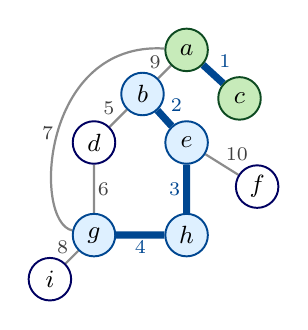
\begin{tikzpicture}[scale=0.56,every node/.append style={font=\footnotesize}]
  \node[gv,comp1] (a) at (3.1,5.2) {$a$};
  \node[gv,comp2] (b) at (2.1,4.2) {$b$};
  \node[gv,comp1] (c) at (4.3,4.1) {$c$};
  \node[gv] (d) at (1.0,3.1) {$d$};
  \node[gv,comp2] (e) at (3.1,3.1) {$e$};
  \node[gv] (f) at (4.7,2.1) {$f$};
  \node[gv,comp2] (g) at (1.0,1.0) {$g$};
  \node[gv,comp2] (h) at (3.1,1.0) {$h$};
  \node[gv] (i) at (0.0,0.0) {$i$};
  \begin{scope}[on background layer]
  \draw[mst] (a) -- node[gw,above right]{1} (c);
  \draw[mst] (b) -- node[gw,above right]{2} (e);
  \draw[mst] (e) -- node[gw,left]{3} (h);
  \draw[mst] (g) -- node[gw,below]{4} (h);
  \draw[ge] (b) -- node[gw,above left]{5} (d);
  \draw[ge] (d) -- node[gw,right]{6} (g);
  \draw[ge] (a) .. controls (-0.2,5.4) and (-0.4,1.3) .. node[gw,left,pos=0.5]{7} (g);
  \draw[ge] (g) -- node[gw,above left]{8} (i);
  \draw[ge] (a) -- node[gw,above left]{9} (b);
  \draw[ge] (e) -- node[gw,above right]{10} (f);
  \end{scope}
\end{tikzpicture}\par
\footnotesize En \emph{skog}: $\{a,c\}$ och $\{b,e,g,h\}$ (och tre ensamma hörn).
\end{column}
\begin{column}{0.33\textwidth}
\centering
{\small\bfseries\color{kthblue}Prim, 4 kanter}\par
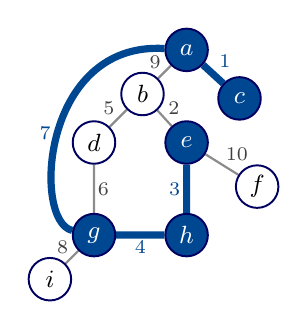
\begin{tikzpicture}[scale=0.56,every node/.append style={font=\footnotesize}]
  \node[gv,intree] (a) at (3.1,5.2) {$a$};
  \node[gv] (b) at (2.1,4.2) {$b$};
  \node[gv,intree] (c) at (4.3,4.1) {$c$};
  \node[gv] (d) at (1.0,3.1) {$d$};
  \node[gv,intree] (e) at (3.1,3.1) {$e$};
  \node[gv] (f) at (4.7,2.1) {$f$};
  \node[gv,intree] (g) at (1.0,1.0) {$g$};
  \node[gv,intree] (h) at (3.1,1.0) {$h$};
  \node[gv] (i) at (0.0,0.0) {$i$};
  \begin{scope}[on background layer]
  \draw[mst] (a) -- node[gw,above right]{1} (c);
  \draw[ge] (b) -- node[gw,above right]{2} (e);
  \draw[mst] (e) -- node[gw,left]{3} (h);
  \draw[mst] (g) -- node[gw,below]{4} (h);
  \draw[ge] (b) -- node[gw,above left]{5} (d);
  \draw[ge] (d) -- node[gw,right]{6} (g);
  \draw[mst] (a) .. controls (-0.2,5.4) and (-0.4,1.3) .. node[gw,left,pos=0.5]{7} (g);
  \draw[ge] (g) -- node[gw,above left]{8} (i);
  \draw[ge] (a) -- node[gw,above left]{9} (b);
  \draw[ge] (e) -- node[gw,above right]{10} (f);
  \end{scope}
\end{tikzpicture}\par
\footnotesize Ett \emph{träd}: $\{a,c,g,h,e\}$.
\end{column}
\begin{column}{0.3\textwidth}
\footnotesize
\textbf{Gemensam invariant:} de valda kanterna är en delmängd av något MST.\par\smallskip
Invarianten är samma. Formen är olika. En tentafråga som visar ett mellantillstånd
avslöjar direkt vilken algoritm som körts.
\end{column}
\end{columns}
\varstrip{Kontrast}{grafen, antal kanter}{algoritmen}{skog (Kruskal) mot sammanhängande träd (Prim)}
\end{frame}

% ---- s2-flow.tex ----
% ======================================================================
%  UPPGIFT 2: FÖRÄNDRAT FLÖDE
% ======================================================================
\section{2 Förändrat flöde}

\uppgiftsbild{2}{Förändrat flöde}
{uppdatera ett maximalt flöde när en kapacitet ändras med 1 — i linjär tid, utan att börja om.}
{\begin{itemize}\setlength{\itemsep}{1pt}
  \item Vad lösningen $\Phi$ \emph{är}: flödet på varje kant, inte bara värdet.
  \item Riktningen: ökning (högst $+1$) mot minskning (högst $-1$).
  \item Kanten: mättad eller inte — och ligger den i \emph{alla} eller i \emph{något} minsnitt?
  \item ”Linjär tid”: linjär i \emph{vad}?
\end{itemize}}

% ---- gen/ff-walk.tex ----
\begin{frame}{Repetition: Ford--Fulkerson på exempelnätet}
\begin{columns}[T]
\begin{column}{0.49\textwidth}
\centering
{\small\bfseries\color{kthnavy}Flöde $f$}\ {\scriptsize(flöde/kapacitet, \textcolor{brick}{röd} = mättad)}\par\smallskip
\only<1>{%
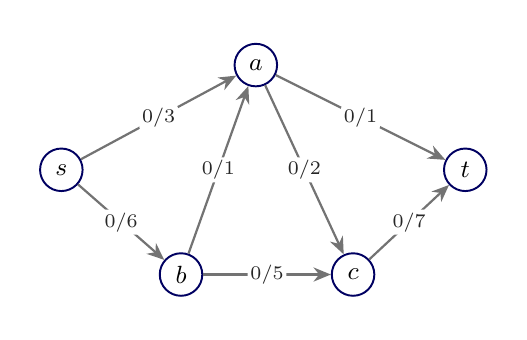
\begin{tikzpicture}[scale=0.95]
\useasboundingbox (-0.45,-0.5) rectangle (5.85,3.3);
  \node[fn] (s) at (0,1.4) {$s$};
  \node[fn] (a) at (2.6,2.8) {$a$};
  \node[fn] (b) at (1.6,0) {$b$};
  \node[fn] (c) at (3.9,0) {$c$};
  \node[fn] (t) at (5.4,1.4) {$t$};
  \draw[fe] (s) -- node[fl] {0/3} (a);
  \draw[fe] (s) -- node[fl] {0/6} (b);
  \draw[fe] (b) -- node[fl] {0/1} (a);
  \draw[fe] (a) -- node[fl] {0/1} (t);
  \draw[fe] (a) -- node[fl] {0/2} (c);
  \draw[fe] (b) -- node[fl] {0/5} (c);
  \draw[fe] (c) -- node[fl] {0/7} (t);
\end{tikzpicture}}
\only<2>{%
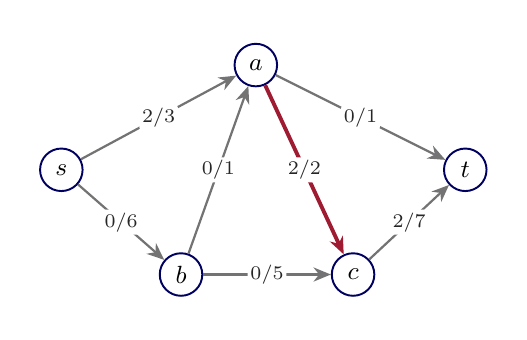
\begin{tikzpicture}[scale=0.95]
\useasboundingbox (-0.45,-0.5) rectangle (5.85,3.3);
  \node[fn] (s) at (0,1.4) {$s$};
  \node[fn] (a) at (2.6,2.8) {$a$};
  \node[fn] (b) at (1.6,0) {$b$};
  \node[fn] (c) at (3.9,0) {$c$};
  \node[fn] (t) at (5.4,1.4) {$t$};
  \draw[fe] (s) -- node[fl] {2/3} (a);
  \draw[fe] (s) -- node[fl] {0/6} (b);
  \draw[fe] (b) -- node[fl] {0/1} (a);
  \draw[fe] (a) -- node[fl] {0/1} (t);
  \draw[sat] (a) -- node[fl] {2/2} (c);
  \draw[fe] (b) -- node[fl] {0/5} (c);
  \draw[fe] (c) -- node[fl] {2/7} (t);
\end{tikzpicture}}
\only<3>{%
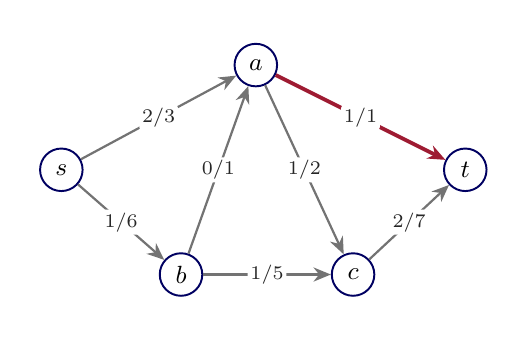
\begin{tikzpicture}[scale=0.95]
\useasboundingbox (-0.45,-0.5) rectangle (5.85,3.3);
  \node[fn] (s) at (0,1.4) {$s$};
  \node[fn] (a) at (2.6,2.8) {$a$};
  \node[fn] (b) at (1.6,0) {$b$};
  \node[fn] (c) at (3.9,0) {$c$};
  \node[fn] (t) at (5.4,1.4) {$t$};
  \draw[fe] (s) -- node[fl] {2/3} (a);
  \draw[fe] (s) -- node[fl] {1/6} (b);
  \draw[fe] (b) -- node[fl] {0/1} (a);
  \draw[sat] (a) -- node[fl] {1/1} (t);
  \draw[fe] (a) -- node[fl] {1/2} (c);
  \draw[fe] (b) -- node[fl] {1/5} (c);
  \draw[fe] (c) -- node[fl] {2/7} (t);
\end{tikzpicture}}
\only<4>{%
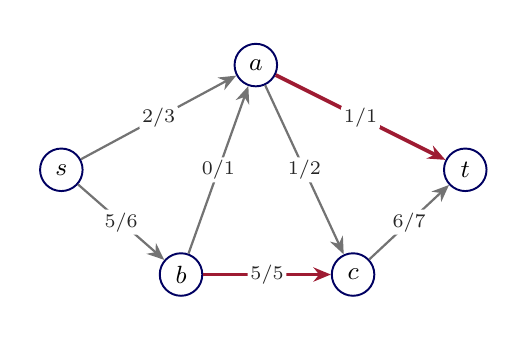
\begin{tikzpicture}[scale=0.95]
\useasboundingbox (-0.45,-0.5) rectangle (5.85,3.3);
  \node[fn] (s) at (0,1.4) {$s$};
  \node[fn] (a) at (2.6,2.8) {$a$};
  \node[fn] (b) at (1.6,0) {$b$};
  \node[fn] (c) at (3.9,0) {$c$};
  \node[fn] (t) at (5.4,1.4) {$t$};
  \draw[fe] (s) -- node[fl] {2/3} (a);
  \draw[fe] (s) -- node[fl] {5/6} (b);
  \draw[fe] (b) -- node[fl] {0/1} (a);
  \draw[sat] (a) -- node[fl] {1/1} (t);
  \draw[fe] (a) -- node[fl] {1/2} (c);
  \draw[sat] (b) -- node[fl] {5/5} (c);
  \draw[fe] (c) -- node[fl] {6/7} (t);
\end{tikzpicture}}
\only<5>{%
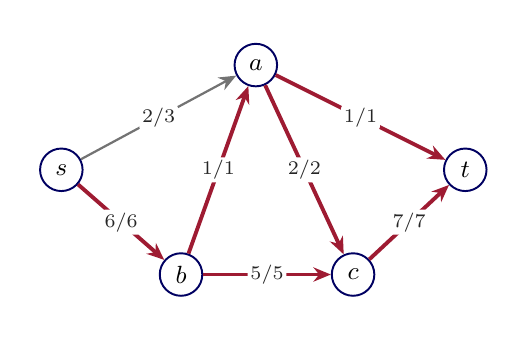
\begin{tikzpicture}[scale=0.95]
\useasboundingbox (-0.45,-0.5) rectangle (5.85,3.3);
  \node[fn] (s) at (0,1.4) {$s$};
  \node[fn] (a) at (2.6,2.8) {$a$};
  \node[fn] (b) at (1.6,0) {$b$};
  \node[fn] (c) at (3.9,0) {$c$};
  \node[fn] (t) at (5.4,1.4) {$t$};
  \draw[fe] (s) -- node[fl] {2/3} (a);
  \draw[sat] (s) -- node[fl] {6/6} (b);
  \draw[sat] (b) -- node[fl] {1/1} (a);
  \draw[sat] (a) -- node[fl] {1/1} (t);
  \draw[sat] (a) -- node[fl] {2/2} (c);
  \draw[sat] (b) -- node[fl] {5/5} (c);
  \draw[sat] (c) -- node[fl] {7/7} (t);
\end{tikzpicture}}
\end{column}
\begin{column}{0.49\textwidth}
\centering
{\small\bfseries\color{kthnavy}Restflödesgraf $G_f$}\ {\scriptsize(\textcolor{kthblue}{kvar}, \textcolor{kthorange}{ångra})}\par\smallskip
\only<1>{%
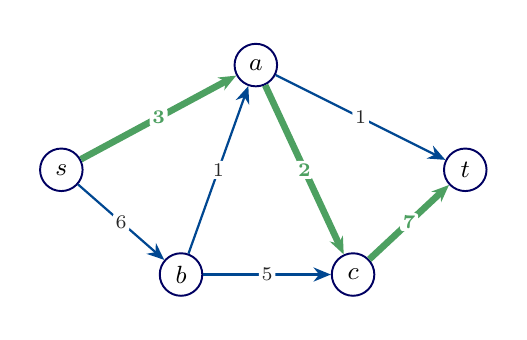
\begin{tikzpicture}[scale=0.95]
\useasboundingbox (-0.45,-0.5) rectangle (5.85,3.3);
  \node[fn] (s) at (0,1.4) {$s$};
  \node[fn] (a) at (2.6,2.8) {$a$};
  \node[fn] (b) at (1.6,0) {$b$};
  \node[fn] (c) at (3.9,0) {$c$};
  \node[fn] (t) at (5.4,1.4) {$t$};
  \draw[aug] (s) -- node[fl,text=kthgrass,font=\scriptsize\bfseries] {3} (a);
  \draw[res] (s) -- node[fl] {6} (b);
  \draw[res] (b) -- node[fl] {1} (a);
  \draw[res] (a) -- node[fl] {1} (t);
  \draw[aug] (a) -- node[fl,text=kthgrass,font=\scriptsize\bfseries] {2} (c);
  \draw[res] (b) -- node[fl] {5} (c);
  \draw[aug] (c) -- node[fl,text=kthgrass,font=\scriptsize\bfseries] {7} (t);
\end{tikzpicture}}
\only<2>{%
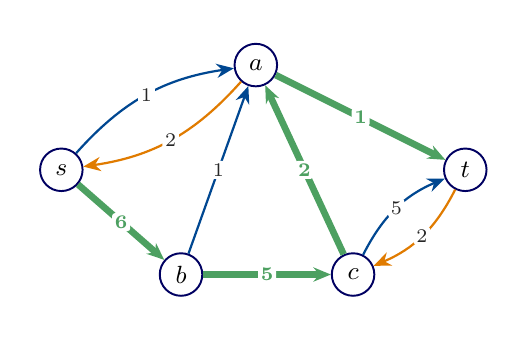
\begin{tikzpicture}[scale=0.95]
\useasboundingbox (-0.45,-0.5) rectangle (5.85,3.3);
  \node[fn] (s) at (0,1.4) {$s$};
  \node[fn] (a) at (2.6,2.8) {$a$};
  \node[fn] (b) at (1.6,0) {$b$};
  \node[fn] (c) at (3.9,0) {$c$};
  \node[fn] (t) at (5.4,1.4) {$t$};
  \draw[res] (s) to[bend left=20] node[fl] {1} (a);
  \draw[resb] (a) to[bend left=20] node[fl] {2} (s);
  \draw[aug] (s) -- node[fl,text=kthgrass,font=\scriptsize\bfseries] {6} (b);
  \draw[res] (b) -- node[fl] {1} (a);
  \draw[aug] (a) -- node[fl,text=kthgrass,font=\scriptsize\bfseries] {1} (t);
  \draw[aug] (c) -- node[fl,text=kthgrass,font=\scriptsize\bfseries] {2} (a);
  \draw[aug] (b) -- node[fl,text=kthgrass,font=\scriptsize\bfseries] {5} (c);
  \draw[res] (c) to[bend left=20] node[fl] {5} (t);
  \draw[resb] (t) to[bend left=20] node[fl] {2} (c);
\end{tikzpicture}}
\only<3>{%
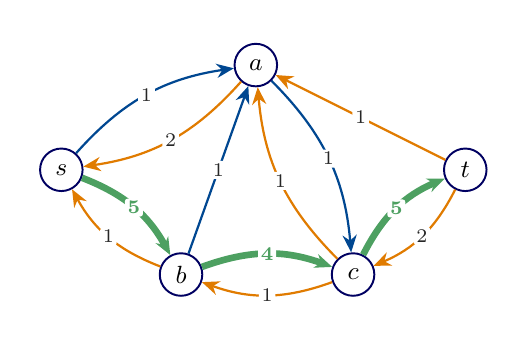
\begin{tikzpicture}[scale=0.95]
\useasboundingbox (-0.45,-0.5) rectangle (5.85,3.3);
  \node[fn] (s) at (0,1.4) {$s$};
  \node[fn] (a) at (2.6,2.8) {$a$};
  \node[fn] (b) at (1.6,0) {$b$};
  \node[fn] (c) at (3.9,0) {$c$};
  \node[fn] (t) at (5.4,1.4) {$t$};
  \draw[res] (s) to[bend left=20] node[fl] {1} (a);
  \draw[resb] (a) to[bend left=20] node[fl] {2} (s);
  \draw[aug] (s) to[bend left=20] node[fl,text=kthgrass,font=\scriptsize\bfseries] {5} (b);
  \draw[resb] (b) to[bend left=20] node[fl] {1} (s);
  \draw[res] (b) -- node[fl] {1} (a);
  \draw[resb] (t) -- node[fl] {1} (a);
  \draw[res] (a) to[bend left=20] node[fl] {1} (c);
  \draw[resb] (c) to[bend left=20] node[fl] {1} (a);
  \draw[aug] (b) to[bend left=20] node[fl,text=kthgrass,font=\scriptsize\bfseries] {4} (c);
  \draw[resb] (c) to[bend left=20] node[fl] {1} (b);
  \draw[aug] (c) to[bend left=20] node[fl,text=kthgrass,font=\scriptsize\bfseries] {5} (t);
  \draw[resb] (t) to[bend left=20] node[fl] {2} (c);
\end{tikzpicture}}
\only<4>{%
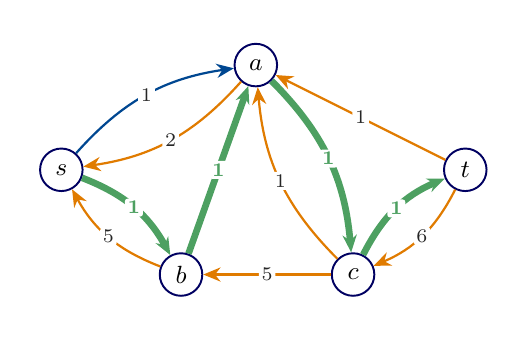
\begin{tikzpicture}[scale=0.95]
\useasboundingbox (-0.45,-0.5) rectangle (5.85,3.3);
  \node[fn] (s) at (0,1.4) {$s$};
  \node[fn] (a) at (2.6,2.8) {$a$};
  \node[fn] (b) at (1.6,0) {$b$};
  \node[fn] (c) at (3.9,0) {$c$};
  \node[fn] (t) at (5.4,1.4) {$t$};
  \draw[res] (s) to[bend left=20] node[fl] {1} (a);
  \draw[resb] (a) to[bend left=20] node[fl] {2} (s);
  \draw[aug] (s) to[bend left=20] node[fl,text=kthgrass,font=\scriptsize\bfseries] {1} (b);
  \draw[resb] (b) to[bend left=20] node[fl] {5} (s);
  \draw[aug] (b) -- node[fl,text=kthgrass,font=\scriptsize\bfseries] {1} (a);
  \draw[resb] (t) -- node[fl] {1} (a);
  \draw[aug] (a) to[bend left=20] node[fl,text=kthgrass,font=\scriptsize\bfseries] {1} (c);
  \draw[resb] (c) to[bend left=20] node[fl] {1} (a);
  \draw[resb] (c) -- node[fl] {5} (b);
  \draw[aug] (c) to[bend left=20] node[fl,text=kthgrass,font=\scriptsize\bfseries] {1} (t);
  \draw[resb] (t) to[bend left=20] node[fl] {6} (c);
\end{tikzpicture}}
\only<5>{%
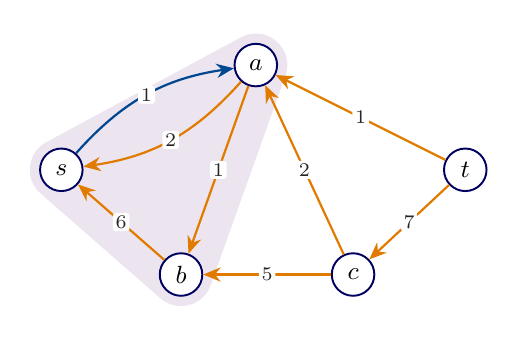
\begin{tikzpicture}[scale=0.95]
\useasboundingbox (-0.45,-0.5) rectangle (5.85,3.3);
  \node[fn] (s) at (0,1.4) {$s$};
  \node[fn] (a) at (2.6,2.8) {$a$};
  \node[fn] (b) at (1.6,0) {$b$};
  \node[fn] (c) at (3.9,0) {$c$};
  \node[fn] (t) at (5.4,1.4) {$t$};
  \begin{scope}[on background layer]
  \filldraw[plum!13,line width=0.8cm,line join=round] (0,1.4) -- (1.6,0) -- (2.6,2.8) -- cycle;
  \end{scope}
  \draw[res] (s) to[bend left=20] node[fl] {1} (a);
  \draw[resb] (a) to[bend left=20] node[fl] {2} (s);
  \draw[resb] (b) -- node[fl] {6} (s);
  \draw[resb] (a) -- node[fl] {1} (b);
  \draw[resb] (t) -- node[fl] {1} (a);
  \draw[resb] (c) -- node[fl] {2} (a);
  \draw[resb] (c) -- node[fl] {5} (b);
  \draw[resb] (t) -- node[fl] {7} (c);
\end{tikzpicture}}
\end{column}
\end{columns}
\vfill
\begin{tcolorbox}[enhanced,halign=left,colback=kthlight!50,colframe=kthsky,boxrule=0.4pt,arc=2pt,
  left=4pt,right=4pt,top=1pt,bottom=1pt,fontupper=\small,height=1.05cm,valign=center]
\only<1>{Inget flöde än: restgrafen är bara kapaciteterna. Välj en stig, vilken som helst: $s\to a\to c\to t$, flaskhals $\min(3,2,7)=2$.}\only<2>{$|f|=2$. Bakåtkanten $c\to a$ (orange) betyder ”ångra flöde på $a\to c$”. Stig $s\to b\to c\to a\to t$ använder den: $+1$.}\only<3>{$|f|=3$. Stig $s\to b\to c\to t$, flaskhals $\min(5,4,5)=4$.}\only<4>{$|f|=7$. Stig $s\to b\to a\to c\to t$, flaskhals 1.}\only<5>{$|f|=8$. Ingen stig $s\leadsto t$ i $G_f$. Nåbara från $s$: $\{s,a,b\}$ — ett minsnitt med kapacitet $1+2+5=8$.}
\end{tcolorbox}
\end{frame}


\begin{frame}{Repetition: maxflöde = minsnitt}
\begin{columns}[T]
\begin{column}{0.44\textwidth}
\centering
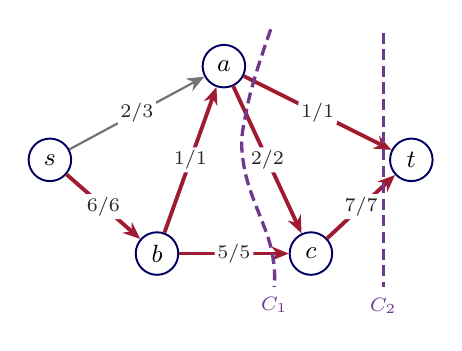
\begin{tikzpicture}[scale=0.85]
  \node[fn] (s) at (0,1.4) {$s$};
  \node[fn] (a) at (2.6,2.8) {$a$};
  \node[fn] (b) at (1.6,0) {$b$};
  \node[fn] (c) at (3.9,0) {$c$};
  \node[fn] (t) at (5.4,1.4) {$t$};
  \draw[fe] (s) -- node[fl] {2/3} (a);
  \draw[sat] (s) -- node[fl] {6/6} (b);
  \draw[sat] (b) -- node[fl] {1/1} (a);
  \draw[sat] (a) -- node[fl] {1/1} (t);
  \draw[sat] (a) -- node[fl] {2/2} (c);
  \draw[sat] (b) -- node[fl] {5/5} (c);
  \draw[sat] (c) -- node[fl] {7/7} (t);
  \draw[cutline] plot[smooth,tension=0.7] coordinates {(3.3,3.35) (2.95,2.2) (2.9,1.3) (3.3,0.1) (3.35,-0.5)};
  \node[below,font=\scriptsize\bfseries,text=plum] at (3.35,-0.5) {$C_1$};
  \draw[cutline] (4.98,3.3) -- (4.98,-0.5) node[below,font=\scriptsize\bfseries,text=plum] {$C_2$};
\end{tikzpicture}\par\smallskip
\footnotesize Två minsnitt, $C_1$ och $C_2$, båda 8.\\ Att de är två kommer att spela roll.
\end{column}
\begin{column}{0.53\textwidth}
\footnotesize
\renewcommand{\arraystretch}{1.1}
\begin{tabular}{@{}lll@{}}
\toprule
$S$ ($s$-sidan) & kanter $S\to T$ & kapacitet\\
\midrule
$\{s\}$ & $s{\to}a$, $s{\to}b$ & $3+6=9$\\
$\{s,a\}$ & $s{\to}b$, $a{\to}t$, $a{\to}c$ & $6+1+2=9$\\
$\{s,b\}$ & $s{\to}a$, $b{\to}a$, $b{\to}c$ & $3+1+5=9$\\
$\{s,c\}$ & $s{\to}a$, $s{\to}b$, $c{\to}t$ & $3+6+7=16$\\
\rowcolor{plum!12} $\{s,a,b\}$ & $a{\to}t$, $a{\to}c$, $b{\to}c$ & $1+2+5=\mathbf{8}$\enspace$C_1$\\
$\{s,a,c\}$ & $s{\to}b$, $a{\to}t$, $c{\to}t$ & $6+1+7=14$\\
$\{s,b,c\}$ & $s{\to}a$, $b{\to}a$, $c{\to}t$ & $3+1+7=11$\\
\rowcolor{plum!12} $\{s,a,b,c\}$ & $a{\to}t$, $c{\to}t$ & $1+7=\mathbf{8}$\enspace$C_2$\\
\bottomrule
\end{tabular}
\end{column}
\end{columns}
\vfill
\begin{missbox}
”Snittets kapacitet är summan av kanterna som korsar det.” Bara kanterna från $S$ till $T$
räknas. För $S=\{s,a\}$ korsar $b\to a$ snittet baklänges och räknas inte.
\end{missbox}
\end{frame}

\begin{frame}{Uppgift 2: Förändrat flöde}
\begin{infobox}
Anta att vi har en lösning $\Phi$ till flödesproblemet för en graf. Beskriv en effektiv algoritm
som hittar ett nytt maximalt flöde om kapaciteten längs en viss kant \textbf{a)}~ökar med en enhet,
\textbf{b)}~minskar med en enhet. Tidskomplexiteten ska vara linjär, alltså $O(|V|+|E|)$.
\end{infobox}
{\small\textbf{Vad består $\Phi$ av?} Två maximala flöden i samma nät:}\par
\begin{columns}[T]
\begin{column}{0.32\textwidth}
\centering
{\footnotesize\bfseries\color{kthnavy}$\Phi_1$, värde 8}\par
% ---- gen/f2.tex ----
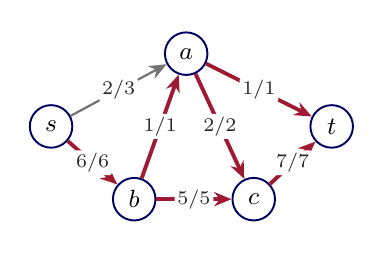
\begin{tikzpicture}[scale=0.66]
\useasboundingbox (-0.45,-0.5) rectangle (5.85,3.3);
  \node[fn] (s) at (0,1.4) {$s$};
  \node[fn] (a) at (2.6,2.8) {$a$};
  \node[fn] (b) at (1.6,0) {$b$};
  \node[fn] (c) at (3.9,0) {$c$};
  \node[fn] (t) at (5.4,1.4) {$t$};
  \draw[fe] (s) -- node[fl] {2/3} (a);
  \draw[sat] (s) -- node[fl] {6/6} (b);
  \draw[sat] (b) -- node[fl] {1/1} (a);
  \draw[sat] (a) -- node[fl] {1/1} (t);
  \draw[sat] (a) -- node[fl] {2/2} (c);
  \draw[sat] (b) -- node[fl] {5/5} (c);
  \draw[sat] (c) -- node[fl] {7/7} (t);
\end{tikzpicture}

\end{column}
\begin{column}{0.32\textwidth}
\centering
{\footnotesize\bfseries\color{kthnavy}$\Phi_2$, värde 8}\par
% ---- gen/fstar.tex ----
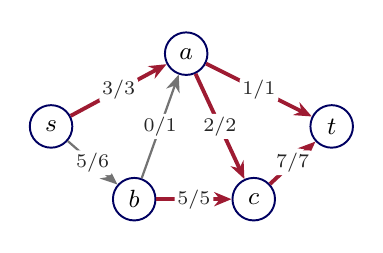
\begin{tikzpicture}[scale=0.66]
\useasboundingbox (-0.45,-0.5) rectangle (5.85,3.3);
  \node[fn] (s) at (0,1.4) {$s$};
  \node[fn] (a) at (2.6,2.8) {$a$};
  \node[fn] (b) at (1.6,0) {$b$};
  \node[fn] (c) at (3.9,0) {$c$};
  \node[fn] (t) at (5.4,1.4) {$t$};
  \draw[sat] (s) -- node[fl] {3/3} (a);
  \draw[fe] (s) -- node[fl] {5/6} (b);
  \draw[fe] (b) -- node[fl] {0/1} (a);
  \draw[sat] (a) -- node[fl] {1/1} (t);
  \draw[sat] (a) -- node[fl] {2/2} (c);
  \draw[sat] (b) -- node[fl] {5/5} (c);
  \draw[sat] (c) -- node[fl] {7/7} (t);
\end{tikzpicture}

\end{column}
\begin{column}{0.31\textwidth}
\footnotesize
Samma värde. Olika flöden: $s{\to}a$ 2 mot 3, $s{\to}b$ 6 mot 5, $b{\to}a$ 1 mot 0.\par\smallskip
$\Phi$ är flödet $f(e)$ \emph{på varje kant}. Med bara talet 8 finns inget att uppdatera — då
återstår att räkna om från början.
\end{column}
\end{columns}
\varstrip{Kontrast}{nätet och värdet 8}{flödet på kanterna}{att $\Phi$ är en funktion på kanterna, inte ett tal}
\end{frame}

% ---------------------------------------------------------------- linjär i vad
\begin{frame}{Linjär i vad?}
\begin{columns}[T]
\begin{column}{0.22\textwidth}
\centering
{\footnotesize\bfseries\color{kthnavy}Grafen}\par\smallskip
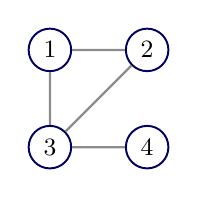
\begin{tikzpicture}[scale=0.95]
  \node[gv] (1) at (0,1.3) {1}; \node[gv] (2) at (1.3,1.3) {2};
  \node[gv] (3) at (0,0) {3};   \node[gv] (4) at (1.3,0) {4};
  \draw[ge] (1)--(2) (1)--(3) (2)--(3) (3)--(4);
\end{tikzpicture}\par
{\scriptsize $|V|=4$, $|E|=4$}
\end{column}
\begin{column}{0.36\textwidth}
\centering
{\footnotesize\bfseries\color{kthnavy}Grannlistor: $|V|+2|E|=12$ platser}\par\smallskip
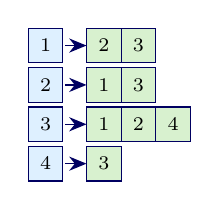
\begin{tikzpicture}[cell/.style={draw=kthnavy,minimum width=4.4mm,minimum height=4.4mm,
    inner sep=0pt,font=\scriptsize},head/.style={cell,fill=kthlight},ent/.style={cell,fill=kthmint!70}]
  \foreach \v/\ns [count=\r] in {1/{2,3},2/{1,3},3/{1,2,4},4/{3}} {
    \node[head] at (0,-0.5*\r) {\v};
    \draw[->,kthnavy,line width=0.5pt] (0.25,-0.5*\r) -- (0.52,-0.5*\r);
    \foreach \n [count=\k] in \ns { \node[ent] at (0.3+0.44*\k,-0.5*\r) {\n}; }
  }
\end{tikzpicture}
\end{column}
\begin{column}{0.36\textwidth}
\centering
{\footnotesize\bfseries\color{kthnavy}Grannmatris: $|V|^2=16$ platser}\par\smallskip
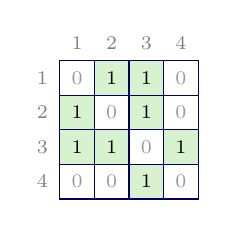
\begin{tikzpicture}[cell/.style={draw=kthnavy,minimum width=4.4mm,minimum height=4.4mm,
    inner sep=0pt,font=\scriptsize},c0/.style={fill=white,text=black!40},c1/.style={fill=kthmint!70}]
  \foreach \row [count=\i] in {{0,1,1,0},{1,0,1,0},{1,1,0,1},{0,0,1,0}} {
    \node[font=\scriptsize,text=black!50] at (0,-0.44*\i) {\i};
    \node[font=\scriptsize,text=black!50] at (0.44*\i,0) {\i};
    \foreach \x [count=\j] in \row { \node[cell,c\x] at (0.44*\j,-0.44*\i) {\x}; }
  }
\end{tikzpicture}
\end{column}
\end{columns}
\smallskip
\footnotesize
\begin{itemize}\setlength{\itemsep}{1pt}
  \item \textbf{Linjär tid} = högst en konstant gånger \emph{indatas storlek}. Man hinner läsa
        indata ett fast antal gånger, inte mer.
  \item BFS/DFS läser varje plats en gång: $O(|V|+|E|)$ med grannlistor, $O(|V|^2)$ med
        grannmatris. \emph{Båda är linjära} — i storleken på sin representation.
  \item $O(|V|+|E|)$ är inte ”linjärt i $|V|$”. I en fullständig graf är
        $|E|=\binom{|V|}{2}$, och då är $O(|V|+|E|)=O(|V|^2)$.
\end{itemize}
\varstrip{Separation}{grafen och algoritmen (BFS)}{representationen}{att ”linjär” mäts i indatas storlek}
\end{frame}

\begin{frame}{Linjär i vad? Dagens uppgifter}
\footnotesize
\renewcommand{\arraystretch}{1.2}
\begin{tabularx}{\textwidth}{@{}p{0.17\textwidth}p{0.3\textwidth}p{0.15\textwidth}X@{}}
\toprule
\textbf{Uppgift} & \textbf{Indatas storlek} & \textbf{”Linjärt”} & \textbf{Kommentar}\\
\midrule
2 Förändrat flöde & $|V|+|E|$ (grafen och $\Phi$) & $O(|V|+|E|)$ & ett par grafsökningar\\
3 Eulercykel & $|V|+|E|$ & $O(|V|+|E|)$ & utdata har $|E|+1$ hörn\\
4 Julklappar & $n$ listor à högst $m$ saker & $O(n+nm)$ & ett varv av Ford--Fulkerson; det blir $n$ varv\\
5 Sökning & $n$ sorterade tal & — & $\Theta(\log n)$: läser inte ens all indata\\
6 Lampor & $n$ lampor & $\Theta(n)$ byten & uppgiften vill ha exakt antal: $2n-1$\\
\bottomrule
\end{tabularx}
\medskip
\begin{missbox}
”Eulercykeln hittas i $O(n)$.” (Så står det i äldre övningsbilder.) Om $n=|V|$ är det fel: en graf
med $|V|$ hörn kan ha $\Theta(|V|^2)$ kanter, och alla ska med i cykeln.
\end{missbox}
\varstrip{Separation}{ordet ”linjär”}{storleksmåttet: $|V|+|E|$, $|V|^2$, $n$, antal byten}{att ”linjär” alltid är linjär \emph{i något}}
\end{frame}

{\kaninbg
\begin{frame}{\kh Linjär i ett tal: pseudopolynomisk tid}
\begin{columns}[T]
\begin{column}{0.38\textwidth}
\centering
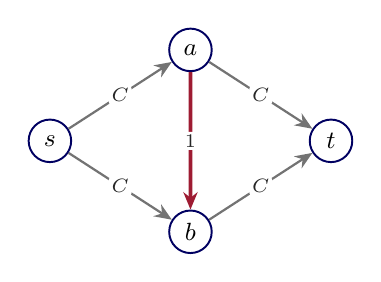
\begin{tikzpicture}[scale=1.05]
  \node[fn] (s) at (0,1.1) {$s$};   \node[fn] (a) at (1.7,2.2) {$a$};
  \node[fn] (b) at (1.7,0) {$b$};   \node[fn] (t) at (3.4,1.1) {$t$};
  \draw[fe] (s) -- node[fl] {$C$} (a);  \draw[fe] (s) -- node[fl] {$C$} (b);
  \draw[fe] (a) -- node[fl] {$C$} (t);  \draw[fe] (b) -- node[fl] {$C$} (t);
  \draw[sat] (a) -- node[fl] {1} (b);
\end{tikzpicture}\par\smallskip
{\footnotesize $C=1\,000\,000\approx2^{20}$}
\end{column}
\begin{column}{0.59\textwidth}
\small
\begin{itemize}\setlength{\itemsep}{2pt}
  \item Ford--Fulkerson väljer stigar godtyckligt. Med otur: varannan stig $s\to a\to b\to t$,
        varannan $s\to b\to a\to t$ (baklänges på $a\to b$).
  \item Varje stig ger $+1$. Maxflödet är $2C$: två miljoner varv.
  \item Indata: fem kanter, tal på cirka 20 bitar. Linjärt i \emph{talet} $C$, exponentiellt
        i antalet \emph{bitar}.
  \item Edmonds--Karp (kortaste stigen först) behöver två varv här, och $O(|V|\,|E|^2)$ i allmänhet.
\end{itemize}
\end{column}
\end{columns}
\vfill
\begin{kaninbox}[fontupper=\footnotesize]
I uppgift 4 är alla kapaciteter 1 och $|f^*|\le n$. Där är $O(|E|\cdot|f^*|)$ helt ofarligt.
\end{kaninbox}
\varstrip{Kontrast}{nätet}{stigvalet: godtyckligt eller kortast}{linjärt i ett tal $\neq$ linjärt i indatas längd}
\end{frame}}

% ---------------------------------------------------------------- 2a
\begin{frame}{2a: kapaciteten på $(u,v)$ ökar med 1}
\begin{columns}[T]
\begin{column}{0.5\textwidth}
\small
\begin{itemize}\setlength{\itemsep}{3pt}
  \item $\Phi$ är fortfarande ett tillåtet flöde: kapaciteten blev ju bara större.
  \item I restflödesgrafen $G_\Phi$ ändras en enda sak: restkapaciteten $u\to v$ ökar med 1.
  \item Kör \textbf{en} iteration av Ford--Fulkerson: sök en stig $s\leadsto t$ i $G_\Phi$.
  \item Finns en stig: öka flödet med 1 längs den. Annars är $\Phi$ fortfarande maximalt.
\end{itemize}
\end{column}
\begin{column}{0.47\textwidth}
{\small\bfseries\color{kthnavy}ÖkaKapacitet$(G,\Phi,(u,v))$}
\footnotesize
\begin{algorithmic}[1]
\State $c(u,v)\gets c(u,v)+1$
\State bygg $G_\Phi$ \Comment{$O(|V|+|E|)$}
\State $P\gets\textsc{BFS}(G_\Phi,s,t)$ \Comment{$O(|V|+|E|)$}
\If{$P$ finns}
  \State öka $\Phi$ med 1 längs $P$ \Comment{$O(|V|)$}
\EndIf
\State \Return $\Phi$
\end{algorithmic}
\end{column}
\end{columns}
\vfill
\begin{columns}[T]
\begin{column}{0.49\textwidth}
\begin{ahabox}[fontupper=\footnotesize]
\textbf{Genväg:} var $(u,v)$ inte mättad händer ingenting. Minsnittet som Ford--Fulkerson hittade
(de nåbara hörnen) har bara mättade kanter ut, så dess kapacitet är oförändrad.
\end{ahabox}
\end{column}
\begin{column}{0.49\textwidth}
\begin{missbox}[fontupper=\footnotesize]
”Kör Ford--Fulkerson igen.” Från början tar det $O(|E|\cdot|f^*|)$ och kastar bort $\Phi$.
\end{missbox}
\end{column}
\end{columns}
\end{frame}

\begin{frame}{2a, exempel: $a\to t$ får kapacitet 2}
\begin{columns}[T]
\begin{column}{0.32\textwidth}
\centering
{\footnotesize\bfseries\color{kthnavy}$\Phi_1$ med ny kapacitet}\par
% ---- gen/2a-net.tex ----
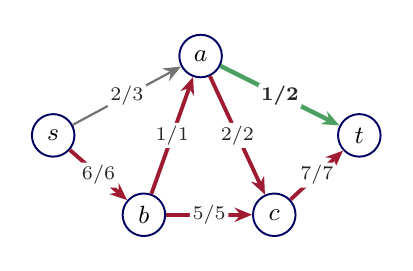
\begin{tikzpicture}[scale=0.72]
\useasboundingbox (-0.45,-0.5) rectangle (5.85,3.3);
  \node[fn] (s) at (0,1.4) {$s$};
  \node[fn] (a) at (2.6,2.8) {$a$};
  \node[fn] (b) at (1.6,0) {$b$};
  \node[fn] (c) at (3.9,0) {$c$};
  \node[fn] (t) at (5.4,1.4) {$t$};
  \draw[fe] (s) -- node[fl] {2/3} (a);
  \draw[sat] (s) -- node[fl] {6/6} (b);
  \draw[sat] (b) -- node[fl] {1/1} (a);
  \draw[->,draw=kthgrass,line width=1.6pt] (a) -- node[fl] {\textbf{1/2}} (t);
  \draw[sat] (a) -- node[fl] {2/2} (c);
  \draw[sat] (b) -- node[fl] {5/5} (c);
  \draw[sat] (c) -- node[fl] {7/7} (t);
\end{tikzpicture}

\end{column}
\begin{column}{0.32\textwidth}
\centering
{\footnotesize\bfseries\color{kthnavy}$G_\Phi$: stigen $s\to a\to t$}\par
% ---- gen/2a-res.tex ----
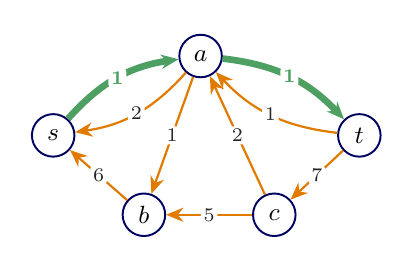
\begin{tikzpicture}[scale=0.72]
\useasboundingbox (-0.45,-0.5) rectangle (5.85,3.3);
  \node[fn] (s) at (0,1.4) {$s$};
  \node[fn] (a) at (2.6,2.8) {$a$};
  \node[fn] (b) at (1.6,0) {$b$};
  \node[fn] (c) at (3.9,0) {$c$};
  \node[fn] (t) at (5.4,1.4) {$t$};
  \draw[aug] (s) to[bend left=20] node[fl,text=kthgrass,font=\scriptsize\bfseries] {1} (a);
  \draw[resb] (a) to[bend left=20] node[fl] {2} (s);
  \draw[resb] (b) -- node[fl] {6} (s);
  \draw[resb] (a) -- node[fl] {1} (b);
  \draw[aug] (a) to[bend left=20] node[fl,text=kthgrass,font=\scriptsize\bfseries] {1} (t);
  \draw[resb] (t) to[bend left=20] node[fl] {1} (a);
  \draw[resb] (c) -- node[fl] {2} (a);
  \draw[resb] (c) -- node[fl] {5} (b);
  \draw[resb] (t) -- node[fl] {7} (c);
\end{tikzpicture}

\end{column}
\begin{column}{0.32\textwidth}
\centering
{\footnotesize\bfseries\color{kthnavy}Nytt flöde, värde 9}\par
% ---- gen/2a-ny.tex ----
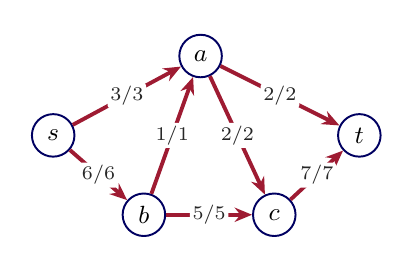
\begin{tikzpicture}[scale=0.72]
\useasboundingbox (-0.45,-0.5) rectangle (5.85,3.3);
  \node[fn] (s) at (0,1.4) {$s$};
  \node[fn] (a) at (2.6,2.8) {$a$};
  \node[fn] (b) at (1.6,0) {$b$};
  \node[fn] (c) at (3.9,0) {$c$};
  \node[fn] (t) at (5.4,1.4) {$t$};
  \draw[sat] (s) -- node[fl] {3/3} (a);
  \draw[sat] (s) -- node[fl] {6/6} (b);
  \draw[sat] (b) -- node[fl] {1/1} (a);
  \draw[sat] (a) -- node[fl] {2/2} (t);
  \draw[sat] (a) -- node[fl] {2/2} (c);
  \draw[sat] (b) -- node[fl] {5/5} (c);
  \draw[sat] (c) -- node[fl] {7/7} (t);
\end{tikzpicture}

\end{column}
\end{columns}
\vfill
\small
Restkanten $a\to t$ (kapacitet 1) är ny, och $s\to a$ hade redan 1 kvar. BFS hittar
$s\to a\to t$. Kanten $a\to t$ ligger i båda minsnitten $C_1$ och $C_2$, så båda växte till 9.
\varstrip{Generalisering}{metoden}{exemplet}{en sökning, en enhet}
\end{frame}

\begin{frame}{2a, exempel: $a\to c$ får kapacitet 3}
\begin{columns}[T]
\begin{column}{0.32\textwidth}
\centering
{\footnotesize\bfseries\color{kthnavy}$\Phi_1$ med ny kapacitet}\par
% ---- gen/2a-ac-net.tex ----
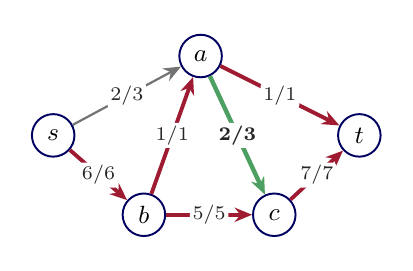
\begin{tikzpicture}[scale=0.72]
\useasboundingbox (-0.45,-0.5) rectangle (5.85,3.3);
  \node[fn] (s) at (0,1.4) {$s$};
  \node[fn] (a) at (2.6,2.8) {$a$};
  \node[fn] (b) at (1.6,0) {$b$};
  \node[fn] (c) at (3.9,0) {$c$};
  \node[fn] (t) at (5.4,1.4) {$t$};
  \draw[fe] (s) -- node[fl] {2/3} (a);
  \draw[sat] (s) -- node[fl] {6/6} (b);
  \draw[sat] (b) -- node[fl] {1/1} (a);
  \draw[sat] (a) -- node[fl] {1/1} (t);
  \draw[->,draw=kthgrass,line width=1.6pt] (a) -- node[fl] {\textbf{2/3}} (c);
  \draw[sat] (b) -- node[fl] {5/5} (c);
  \draw[sat] (c) -- node[fl] {7/7} (t);
\end{tikzpicture}

\end{column}
\begin{column}{0.32\textwidth}
\centering
{\footnotesize\bfseries\color{kthnavy}$G_\Phi$: nåbart från $s$}\par
% ---- gen/2a-res-ac.tex ----
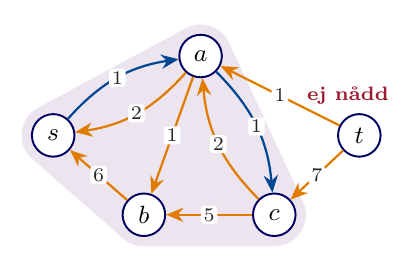
\begin{tikzpicture}[scale=0.72]
\useasboundingbox (-0.45,-0.5) rectangle (5.85,3.3);
  \node[fn] (s) at (0,1.4) {$s$};
  \node[fn] (a) at (2.6,2.8) {$a$};
  \node[fn] (b) at (1.6,0) {$b$};
  \node[fn] (c) at (3.9,0) {$c$};
  \node[fn] (t) at (5.4,1.4) {$t$};
  \begin{scope}[on background layer]
  \filldraw[plum!13,line width=0.8cm,line join=round] (0,1.4) -- (1.6,0) -- (3.9,0) -- (2.6,2.8) -- cycle;
  \end{scope}
  \draw[res] (s) to[bend left=20] node[fl] {1} (a);
  \draw[resb] (a) to[bend left=20] node[fl] {2} (s);
  \draw[resb] (b) -- node[fl] {6} (s);
  \draw[resb] (a) -- node[fl] {1} (b);
  \draw[resb] (t) -- node[fl] {1} (a);
  \draw[res] (a) to[bend left=20] node[fl] {1} (c);
  \draw[resb] (c) to[bend left=20] node[fl] {2} (a);
  \draw[resb] (c) -- node[fl] {5} (b);
  \draw[resb] (t) -- node[fl] {7} (c);
  \node[font=\scriptsize\bfseries,text=brick] at (5.2,2.1) {ej nådd};
\end{tikzpicture}

\end{column}
\begin{column}{0.32\textwidth}
\small
Nu nås $c$ via $s\to a\to c$ — men $c\to t$ är mättad. $t$ nås inte.\par\medskip
$\Phi_1$ är fortfarande maximalt: 8. Minsnittet $C_2=\{s,a,b,c\}$ innehåller inte $a\to c$
och har kvar kapaciteten 8.
\end{column}
\end{columns}
\vfill
\begin{missbox}
”Kanten var mättad, alltså hjälper det att öka den.” Mättad är nödvändigt men inte tillräckligt.
\end{missbox}
\varstrip{Kontrast}{nätet och $\Phi_1$}{vilken mättad kant som ökas}{att en ökning kan vara verkningslös}
\end{frame}

{\kaninbg
\begin{frame}{\kh Varför räcker en enda sökning?}
\begin{columns}[T]
\begin{column}{0.56\textwidth}
\small
\begin{itemize}\setlength{\itemsep}{3pt}
  \item Ett snitts kapacitet är summan av kanterna $S\to T$. När $c(u,v)$ ökar med 1 växer
        varje snitt med 1 (om $u\in S$, $v\in T$) eller med 0.
  \item Maxflöde = minsnitt, så det nya maxflödet är högst $|\Phi|+1$.
  \item Allt är heltal: antingen samma eller exakt $+1$. En förbättrande stig, sedan är vi klara.
  \item Ingen stig? Då är $\Phi$ maximalt. Det är Ford--Fulkersons eget stoppvillkor.
\end{itemize}
\end{column}
\begin{column}{0.41\textwidth}
\centering
% ---- gen/minsnitt-s.tex ----
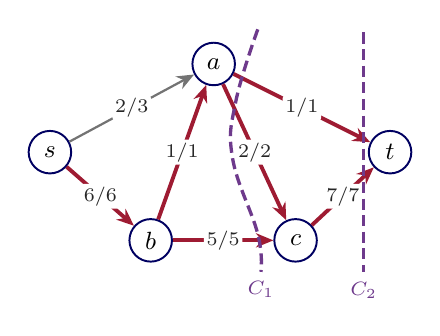
\begin{tikzpicture}[scale=0.8]
  \node[fn] (s) at (0,1.4) {$s$};
  \node[fn] (a) at (2.6,2.8) {$a$};
  \node[fn] (b) at (1.6,0) {$b$};
  \node[fn] (c) at (3.9,0) {$c$};
  \node[fn] (t) at (5.4,1.4) {$t$};
  \draw[fe] (s) -- node[fl] {2/3} (a);
  \draw[sat] (s) -- node[fl] {6/6} (b);
  \draw[sat] (b) -- node[fl] {1/1} (a);
  \draw[sat] (a) -- node[fl] {1/1} (t);
  \draw[sat] (a) -- node[fl] {2/2} (c);
  \draw[sat] (b) -- node[fl] {5/5} (c);
  \draw[sat] (c) -- node[fl] {7/7} (t);
  \draw[cutline] plot[smooth,tension=0.7] coordinates {(3.3,3.35) (2.95,2.2) (2.9,1.3) (3.3,0.1) (3.35,-0.5)};
  \node[below,font=\scriptsize\bfseries,text=plum] at (3.35,-0.5) {$C_1$};
  \draw[cutline] (4.98,3.3) -- (4.98,-0.5) node[below,font=\scriptsize\bfseries,text=plum] {$C_2$};
\end{tikzpicture}

\end{column}
\end{columns}
\vfill
\begin{kaninbox}[fontupper=\footnotesize]
\textbf{Och om kapaciteten ökar med $k$?} Då kan maxflödet öka med upp till $k$, och det kan behövas
$k$ sökningar: $O(k(|V|+|E|))$. Linjärt bara om $k$ är en konstant.
\end{kaninbox}
\end{frame}}

\begin{frame}{Samma ändring, olika kant: när hjälper $+1$?}
\begin{columns}[T]
\begin{column}{0.4\textwidth}
\centering
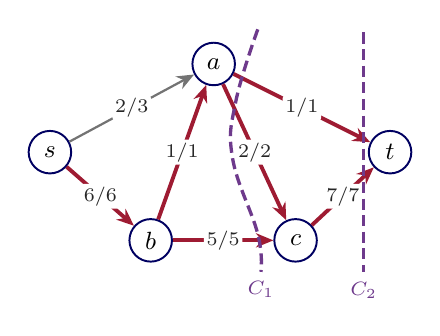
\begin{tikzpicture}[scale=0.8]
  \node[fn] (s) at (0,1.4) {$s$};
  \node[fn] (a) at (2.6,2.8) {$a$};
  \node[fn] (b) at (1.6,0) {$b$};
  \node[fn] (c) at (3.9,0) {$c$};
  \node[fn] (t) at (5.4,1.4) {$t$};
  \draw[fe] (s) -- node[fl] {2/3} (a);
  \draw[sat] (s) -- node[fl] {6/6} (b);
  \draw[sat] (b) -- node[fl] {1/1} (a);
  \draw[sat] (a) -- node[fl] {1/1} (t);
  \draw[sat] (a) -- node[fl] {2/2} (c);
  \draw[sat] (b) -- node[fl] {5/5} (c);
  \draw[sat] (c) -- node[fl] {7/7} (t);
  \draw[cutline] plot[smooth,tension=0.7] coordinates {(3.3,3.35) (2.95,2.2) (2.9,1.3) (3.3,0.1) (3.35,-0.5)};
  \node[below,font=\scriptsize\bfseries,text=plum] at (3.35,-0.5) {$C_1$};
  \draw[cutline] (4.98,3.3) -- (4.98,-0.5) node[below,font=\scriptsize\bfseries,text=plum] {$C_2$};
\end{tikzpicture}\par
\begin{ahabox}[fontupper=\footnotesize]
Maxflödet ökar precis när kanten ligger i \textbf{alla} minsnitt. Ett enda minsnitt utan
kanten håller taket kvar.
\end{ahabox}
\end{column}
\begin{column}{0.57\textwidth}
\footnotesize
\renewcommand{\arraystretch}{1.1}
\begin{tabular}{@{}lccccc@{}}
\toprule
Kant & $\Phi_1$ & mättad & i $C_1$ & i $C_2$ & $+1$ ger\\
\midrule
\rowcolor{kthmint!50} $a{\to}t$ & 1/1 & \ja & \ja & \ja & \textbf{9}\\
$a{\to}c$ & 2/2 & \ja & \ja & & 8\\
$b{\to}c$ & 5/5 & \ja & \ja & & 8\\
$c{\to}t$ & 7/7 & \ja & & \ja & 8\\
$s{\to}b$ & 6/6 & \ja & & & 8\\
$b{\to}a$ & 1/1 & \ja & & & 8\\
$s{\to}a$ & 2/3 & & & & 8\\
\bottomrule
\end{tabular}
\par\smallskip
\begin{missbox}[fontupper=\footnotesize]
”Mättad kant $\Rightarrow$ ökningen hjälper.” Sex av sju kanter är mättade. En hjälper.
\end{missbox}
\end{column}
\end{columns}
\varstrip{Separation}{nätet, $\Phi_1$ och ändringen $+1$}{kanten}{att minsnitten bestämmer, inte mättnaden}
\end{frame}

% ---------------------------------------------------------------- 2b
\begin{frame}{2b: kapaciteten på $(u,v)$ minskar med 1}
\begin{columns}[T]
\begin{column}{0.49\textwidth}
\small
\textbf{Fall 1:} $(u,v)$ är inte mättad. $\Phi$ är fortfarande tillåtet, och maxflödet kan inte
öka när en kapacitet minskar. Klart.\par\smallskip
\textbf{Annars:} minska $\Phi(u,v)$ med 1. Nu kommer det in en enhet mer till $u$ än som går ut,
och en enhet mindre till $v$.\par\smallskip
\textbf{Fall 2:} finns en stig $u\leadsto v$ i $G_\Phi$? Led enheten den vägen. Värdet är
oförändrat.\par\smallskip
\textbf{Fall 3:} annars: skicka tillbaka enheten, $u\leadsto s$, och ta bort en enhet från $v$
till $t$ genom att gå $t\leadsto v$. Värdet minskar med 1.
\end{column}
\begin{column}{0.49\textwidth}
{\small\bfseries\color{kthnavy}MinskaKapacitet$(G,\Phi,(u,v))$}
\footnotesize
\begin{algorithmic}[1]
\State $c(u,v)\gets c(u,v)-1$
\If{$\Phi(u,v)\le c(u,v)$} \State \Return $\Phi$ \Comment{fall 1}
\EndIf
\State $\Phi(u,v)\gets\Phi(u,v)-1$ \Comment{obalans i $u$, $v$}
\If{stig $P\colon u\leadsto v$ finns i $G_\Phi$}
  \State öka $\Phi$ med 1 längs $P$ \Comment{fall 2}
\Else
  \State öka $\Phi$ med 1 längs en stig $u\leadsto s$ \Comment{fall 3}
  \State öka $\Phi$ med 1 längs en stig $t\leadsto v$
\EndIf
\State \Return $\Phi$
\end{algorithmic}
\smallskip
{\footnotesize Högst tre grafsökningar: $O(|V|+|E|)$.}
\end{column}
\end{columns}
\vfill
\begin{missbox}
”Minska flödet på kanten med 1, klart.” Då kommer mer in i $u$ än som går ut. Det är inte längre
ett flöde.
\end{missbox}
\end{frame}

\begin{frame}{2b, exempel (fall 2): $b\to a$ får kapacitet 0}
\begin{columns}[T]
\begin{column}{0.32\textwidth}
\centering
{\footnotesize\bfseries\color{kthnavy}Obalans efter minskningen}\par
% ---- gen/2b-ba-net.tex ----
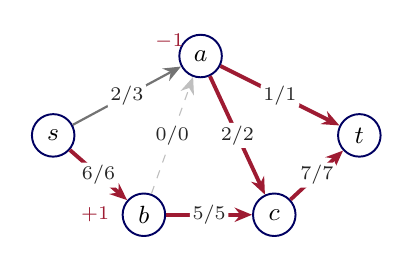
\begin{tikzpicture}[scale=0.72]
\useasboundingbox (-0.45,-0.5) rectangle (5.85,3.3);
  \node[fn] (s) at (0,1.4) {$s$};
  \node[fn] (a) at (2.6,2.8) {$a$};
  \node[fn] (b) at (1.6,0) {$b$};
  \node[fn] (c) at (3.9,0) {$c$};
  \node[fn] (t) at (5.4,1.4) {$t$};
  \draw[fe] (s) -- node[fl] {2/3} (a);
  \draw[sat] (s) -- node[fl] {6/6} (b);
  \draw[->,draw=black!25,dashed] (b) -- node[fl] {0/0} (a);
  \draw[sat] (a) -- node[fl] {1/1} (t);
  \draw[sat] (a) -- node[fl] {2/2} (c);
  \draw[sat] (b) -- node[fl] {5/5} (c);
  \draw[sat] (c) -- node[fl] {7/7} (t);
  \node[font=\scriptsize\bfseries,text=brick,left=1pt of b] {$+1$};
  \node[font=\scriptsize\bfseries,text=brick] at (2.05,3.05) {$-1$};
\end{tikzpicture}

\end{column}
\begin{column}{0.32\textwidth}
\centering
{\footnotesize\bfseries\color{kthnavy}$G_\Phi$: stigen $b\to s\to a$}\par
% ---- gen/2b-ba-res.tex ----
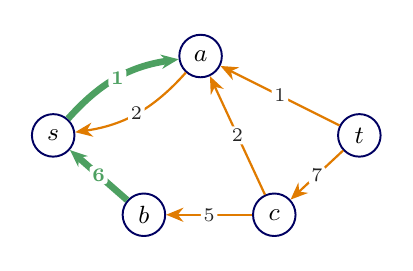
\begin{tikzpicture}[scale=0.72]
\useasboundingbox (-0.45,-0.5) rectangle (5.85,3.3);
  \node[fn] (s) at (0,1.4) {$s$};
  \node[fn] (a) at (2.6,2.8) {$a$};
  \node[fn] (b) at (1.6,0) {$b$};
  \node[fn] (c) at (3.9,0) {$c$};
  \node[fn] (t) at (5.4,1.4) {$t$};
  \draw[aug] (s) to[bend left=20] node[fl,text=kthgrass,font=\scriptsize\bfseries] {1} (a);
  \draw[resb] (a) to[bend left=20] node[fl] {2} (s);
  \draw[aug] (b) -- node[fl,text=kthgrass,font=\scriptsize\bfseries] {6} (s);
  \draw[resb] (t) -- node[fl] {1} (a);
  \draw[resb] (c) -- node[fl] {2} (a);
  \draw[resb] (c) -- node[fl] {5} (b);
  \draw[resb] (t) -- node[fl] {7} (c);
\end{tikzpicture}

\end{column}
\begin{column}{0.32\textwidth}
\centering
{\footnotesize\bfseries\color{kthnavy}Nytt flöde, värde 8}\par
% ---- gen/2b-ba-ny.tex ----
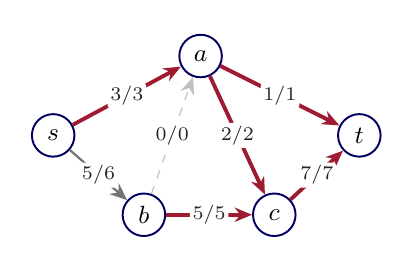
\begin{tikzpicture}[scale=0.72]
\useasboundingbox (-0.45,-0.5) rectangle (5.85,3.3);
  \node[fn] (s) at (0,1.4) {$s$};
  \node[fn] (a) at (2.6,2.8) {$a$};
  \node[fn] (b) at (1.6,0) {$b$};
  \node[fn] (c) at (3.9,0) {$c$};
  \node[fn] (t) at (5.4,1.4) {$t$};
  \draw[sat] (s) -- node[fl] {3/3} (a);
  \draw[fe] (s) -- node[fl] {5/6} (b);
  \draw[->,draw=black!25,dashed] (b) -- node[fl] {0/0} (a);
  \draw[sat] (a) -- node[fl] {1/1} (t);
  \draw[sat] (a) -- node[fl] {2/2} (c);
  \draw[sat] (b) -- node[fl] {5/5} (c);
  \draw[sat] (c) -- node[fl] {7/7} (t);
\end{tikzpicture}

\end{column}
\end{columns}
\vfill
\small
$b$ har en enhet för mycket, $a$ en för lite. Stigen $b\to s\to a$ går baklänges på $s\to b$ och
framlänges på $s\to a$: enheten tar vägen $s\to a$ i stället. Resultatet är $\Phi_2$ — det andra
maxflödet från bilden om vad $\Phi$ är.
\varstrip{Kontrast}{nätet, $\Phi_1$ och minskningen}{kanten (här: ingen i något minsnitt)}{omledning bevarar värdet}
\end{frame}

\begin{frame}{2b, exempel (fall 3): $a\to c$ får kapacitet 1}
\begin{columns}[T]
\begin{column}{0.32\textwidth}
\centering
{\footnotesize\bfseries\color{kthnavy}Obalans efter minskningen}\par
% ---- gen/2b-ac-net.tex ----
\begin{tikzpicture}[scale=0.72]
\useasboundingbox (-0.45,-0.5) rectangle (5.85,3.3);
  \node[fn] (s) at (0,1.4) {$s$};
  \node[fn] (a) at (2.6,2.8) {$a$};
  \node[fn] (b) at (1.6,0) {$b$};
  \node[fn] (c) at (3.9,0) {$c$};
  \node[fn] (t) at (5.4,1.4) {$t$};
  \draw[fe] (s) -- node[fl] {2/3} (a);
  \draw[sat] (s) -- node[fl] {6/6} (b);
  \draw[sat] (b) -- node[fl] {1/1} (a);
  \draw[sat] (a) -- node[fl] {1/1} (t);
  \draw[sat] (a) -- node[fl] {1/1} (c);
  \draw[sat] (b) -- node[fl] {5/5} (c);
  \draw[sat] (c) -- node[fl] {7/7} (t);
  \node[font=\scriptsize\bfseries,text=brick] at (2.05,3.05) {$+1$};
  \node[font=\scriptsize\bfseries,text=brick] at (4.45,-0.25) {$-1$};
\end{tikzpicture}

\end{column}
\begin{column}{0.32\textwidth}
\centering
{\footnotesize\bfseries\color{kthnavy}$G_\Phi$: nåbart från $a$}\par
% ---- gen/2b-ac-res.tex ----
\begin{tikzpicture}[scale=0.72]
\useasboundingbox (-0.45,-0.5) rectangle (5.85,3.3);
  \node[fn] (s) at (0,1.4) {$s$};
  \node[fn] (a) at (2.6,2.8) {$a$};
  \node[fn] (b) at (1.6,0) {$b$};
  \node[fn] (c) at (3.9,0) {$c$};
  \node[fn] (t) at (5.4,1.4) {$t$};
  \begin{scope}[on background layer]
  \filldraw[plum!13,line width=0.8cm,line join=round] (0,1.4) -- (1.6,0) -- (2.6,2.8) -- cycle;
  \end{scope}
  \draw[res] (s) to[bend left=20] node[fl] {1} (a);
  \draw[aug] (a) to[bend left=20] node[fl,text=kthgrass,font=\scriptsize\bfseries] {2} (s);
  \draw[resb] (b) -- node[fl] {6} (s);
  \draw[resb] (a) -- node[fl] {1} (b);
  \draw[resb] (t) -- node[fl] {1} (a);
  \draw[resb] (c) -- node[fl] {1} (a);
  \draw[resb] (c) -- node[fl] {5} (b);
  \draw[aug] (t) -- node[fl,text=kthgrass,font=\scriptsize\bfseries] {7} (c);
\end{tikzpicture}

\end{column}
\begin{column}{0.32\textwidth}
\centering
{\footnotesize\bfseries\color{kthnavy}Nytt flöde, värde 7}\par
% ---- gen/2b-ac-ny.tex ----
\begin{tikzpicture}[scale=0.72]
\useasboundingbox (-0.45,-0.5) rectangle (5.85,3.3);
  \node[fn] (s) at (0,1.4) {$s$};
  \node[fn] (a) at (2.6,2.8) {$a$};
  \node[fn] (b) at (1.6,0) {$b$};
  \node[fn] (c) at (3.9,0) {$c$};
  \node[fn] (t) at (5.4,1.4) {$t$};
  \draw[fe] (s) -- node[fl] {1/3} (a);
  \draw[sat] (s) -- node[fl] {6/6} (b);
  \draw[sat] (b) -- node[fl] {1/1} (a);
  \draw[sat] (a) -- node[fl] {1/1} (t);
  \draw[sat] (a) -- node[fl] {1/1} (c);
  \draw[sat] (b) -- node[fl] {5/5} (c);
  \draw[fe] (c) -- node[fl] {6/7} (t);
\end{tikzpicture}

\end{column}
\end{columns}
\vfill
\small
Från $a$ nås bara $\{a,s,b\}$, inte $c$. Alltså fall 3: skicka tillbaka längs $a\to s$ och ta
bort en enhet längs $t\to c$ (båda baklänges i restgrafen, gröna). Kanten $a\to c$ ligger i
minsnittet $C_1$, som nu har kapacitet 7.
\varstrip{Kontrast}{nätet, $\Phi_1$ och minskningen}{kanten (här: i minsnittet $C_1$)}{när värdet måste sjunka}
\end{frame}

{\kaninbg
\begin{frame}{\kh Varför finns stigarna $u\leadsto s$ och $t\leadsto v$?}
\begin{columns}[T]
\begin{column}{0.57\textwidth}
\small
\begin{itemize}\setlength{\itemsep}{3pt}
  \item \textbf{Flödesuppdelning:} varje flöde är en summa av $s$--$t$-stigar och cykler med
        positivt flöde. $\Phi_1$: $s{\to}b{\to}c{\to}t$ (5), $s{\to}a{\to}c{\to}t$ (2),
        $s{\to}b{\to}a{\to}t$ (1).
  \item $(u,v)$ var mättad, så $\Phi(u,v)\ge1$: någon stig eller cykel går genom $(u,v)$.
  \item \textbf{Stig} $s\leadsto u\to v\leadsto t$: flödet på delarna ger bakåtkanter
        $u\leadsto s$ och $t\leadsto v$ i $G_\Phi$.
  \item \textbf{Cykel} genom $(u,v)$: resten av cykeln, baklänges, är en stig $u\leadsto v$.
        Då var vi i fall 2.
\end{itemize}
\end{column}
\begin{column}{0.4\textwidth}
\centering
{\footnotesize\bfseries\color{kthgrass}$s\to a\to c\to t$ bär 2 enheter}\par
% ---- gen/f2-stig-ac.tex ----
\begin{tikzpicture}[scale=0.8]
\useasboundingbox (-0.45,-0.5) rectangle (5.85,3.3);
  \node[fn] (s) at (0,1.4) {$s$};
  \node[fn] (a) at (2.6,2.8) {$a$};
  \node[fn] (b) at (1.6,0) {$b$};
  \node[fn] (c) at (3.9,0) {$c$};
  \node[fn] (t) at (5.4,1.4) {$t$};
  \draw[aug] (s) -- node[fl] {2/3} (a);
  \draw[fe] (s) -- node[fl] {6/6} (b);
  \draw[fe] (b) -- node[fl] {1/1} (a);
  \draw[fe] (a) -- node[fl] {1/1} (t);
  \draw[aug] (a) -- node[fl] {2/2} (c);
  \draw[fe] (b) -- node[fl] {5/5} (c);
  \draw[aug] (c) -- node[fl] {7/7} (t);
\end{tikzpicture}

\end{column}
\end{columns}
\vfill
\begin{kaninbox}[fontupper=\footnotesize]
Gör sökningarna en i taget: först $u\leadsto s$, uppdatera $\Phi$, sedan $t\leadsto v$ i den nya
restgrafen. Samma uppdelningsargument på det uppdaterade flödet visar att den andra stigen
fortfarande finns.
\end{kaninbox}
\end{frame}}

{\kaninbg
\begin{frame}{\kh Är flödet i fall 3 säkert maximalt?}
\begin{columns}[T]
\begin{column}{0.58\textwidth}
\small
\footnotesize
\begin{itemize}\setlength{\itemsep}{2pt}
  \item Låt $A$ = hörnen som nås från $u$ i $G_\Phi$. Fall 3 betyder $v\notin A$.
  \item $s\in A$, för stigen $u\leadsto s$ finns. $t\notin A$, annars fanns $u\leadsto t\leadsto v$.
  \item Ingen restkant lämnar $A$: kanterna ut ur $A$ är mättade, kanterna in är tomma.
  \item Flödet över snittet är då lika med dess kapacitet, och det är $|\Phi|-1$: enheten som
        blev över i $u$ stannar i $A$.
  \item Tillbakatrycken sker helt inom $A$ respektive helt utanför. Nya flödet har värdet
        $|\Phi|-1$ = ett snitts kapacitet. Alltså maximalt.
\end{itemize}
\end{column}
\begin{column}{0.39\textwidth}
\centering
\begin{tikzpicture}[scale=0.8]
\useasboundingbox (-0.45,-0.5) rectangle (5.85,3.3);
  \node[fn] (s) at (0,1.4) {$s$};
  \node[fn] (a) at (2.6,2.8) {$a$};
  \node[fn] (b) at (1.6,0) {$b$};
  \node[fn] (c) at (3.9,0) {$c$};
  \node[fn] (t) at (5.4,1.4) {$t$};
  \begin{scope}[on background layer]
  \filldraw[plum!13,line width=0.8cm,line join=round] (0,1.4) -- (1.6,0) -- (2.6,2.8) -- cycle;
  \end{scope}
  \node[font=\small\bfseries,text=plum] at (0.35,0.1) {$A$};
  \draw[res] (s) to[bend left=20] node[fl] {1} (a);
  \draw[resb] (a) to[bend left=20] node[fl] {2} (s);
  \draw[resb] (b) -- node[fl] {6} (s);
  \draw[resb] (a) -- node[fl] {1} (b);
  \draw[resb] (t) -- node[fl] {1} (a);
  \draw[resb] (c) -- node[fl] {1} (a);
  \draw[resb] (c) -- node[fl] {5} (b);
  \draw[resb] (t) -- node[fl] {7} (c);
  \draw[cutline] plot[smooth,tension=0.7] coordinates {(3.3,3.35) (2.95,2.2) (2.9,1.3) (3.3,0.1) (3.35,-0.5)};
\end{tikzpicture}\par
{\footnotesize Här: $A=\{s,a,b\}$, och $1+1+5=7$.}
\end{column}
\end{columns}
\vfill
\begin{kaninbox}[fontupper=\footnotesize]
Ingen extra kontroll behövs. (En extra BFS skulle inte förstöra linjäriteten. Den är bara onödig.)
\end{kaninbox}
\end{frame}}

{\kaninbg
\begin{frame}{\kh Alternativ lösning: b) via a)}
\small
Om $(u,v)$ är mättad:
\begin{enumerate}\setlength{\itemsep}{3pt}
  \item \textbf{Ta bort en enhet flöde genom $(u,v)$:} minska $\Phi(u,v)$ och tryck tillbaka
        längs $u\leadsto s$ och $t\leadsto v$. Nu är $\Phi$ tillåtet med den nya kapaciteten och
        har värdet $|\Phi|-1$.
  \item \textbf{Gör som i a):} en sökning $s\leadsto t$. Maxflödet är nu $|\Phi|-1$ eller
        $|\Phi|$, så en förbättrande stig räcker.
\end{enumerate}
\medskip
Exempel $b\to a$: steg 1 tar bort enheten på $s\to b\to a\to t$ (värde 7), steg 2 hittar
$s\to a\to t$ (värde 8). Samma slutresultat, $\Phi_2$.
\vfill
\begin{kaninbox}[fontupper=\footnotesize]
Tre sökningar i stället för en eller två — fortfarande $O(|V|+|E|)$. Vinsten är att
korrekthetsbeviset blir kortare: efter steg 1 är vi exakt i situationen i a).
\end{kaninbox}
\varstrip{Generalisering}{metoden: restgraf och en sökning}{problemet: öka eller minska}{att b) är ”ta bort en enhet” följt av a)}
\end{frame}}

% ---------------------------------------------------------------- fusion
\begin{frame}{Öka och minska, kant för kant}
\begin{columns}[T]
\begin{column}{0.58\textwidth}
\footnotesize
\renewcommand{\arraystretch}{1.02}
\begin{tabular}{@{}lcccccl@{}}
\toprule
Kant & $\Phi_1$ & i $C_1$ & i $C_2$ & $+1$ & $-1$ & fall vid $-1$\\
\midrule
$a{\to}t$ & 1/1 & \ja & \ja & \textbf{9} & \textbf{7} & 3\\
$a{\to}c$ & 2/2 & \ja & & 8 & \textbf{7} & 3\\
$b{\to}c$ & 5/5 & \ja & & 8 & \textbf{7} & 3\\
$c{\to}t$ & 7/7 & & \ja & 8 & \textbf{7} & 3\\
$s{\to}b$ & 6/6 & & & 8 & 8 & 2: $s{\to}a{\to}b$\\
$b{\to}a$ & 1/1 & & & 8 & 8 & 2: $b{\to}s{\to}a$\\
$s{\to}a$ & 2/3 & & & 8 & 8 & 1\\
\bottomrule
\end{tabular}
\end{column}
\begin{column}{0.39\textwidth}
\begin{ahabox}[fontupper=\footnotesize]
$+1$ ökar maxflödet $\iff$ kanten ligger i \textbf{alla} minsnitt.\par\smallskip
$-1$ minskar maxflödet $\iff$ kanten ligger i \textbf{något} minsnitt.
\end{ahabox}
\end{column}
\end{columns}
\vfill
\begin{columns}[T]
\begin{column}{0.49\textwidth}
\begin{missbox}[fontupper=\footnotesize]
”Ökning och minskning är symmetriska.” $a\to c$ kan inte öka maxflödet, men kan minska det.
\end{missbox}
\end{column}
\begin{column}{0.49\textwidth}
\begin{missbox}[fontupper=\footnotesize]
”Mättad är en egenskap hos kanten.” Hos kanten \emph{och} $\Phi$: $s\to b$ är mättad i $\Phi_1$
(6/6) men inte i $\Phi_2$ (5/6).
\end{missbox}
\end{column}
\end{columns}
\varstrip{Fusion}{nätet}{kanten och riktningen samtidigt}{alla mot något minsnitt; mättnad beror på $\Phi$}
\end{frame}

\begin{frame}{Vanliga fel i uppgift 2}
\begin{columns}[T]
\begin{column}{0.49\textwidth}
\begin{missbox}[fontupper=\footnotesize]
”$\Phi$ är ett tal, 8.” Det är flödet på varje kant. Med bara talet måste man räkna om från början.
\end{missbox}
\begin{missbox}[fontupper=\footnotesize]
”Öka flödet på $(u,v)$ med 1.” Då bryts flödesbevarandet i $u$ och $v$, och enheten kanske inte
ens kan komma fram till $t$.
\end{missbox}
\end{column}
\begin{column}{0.49\textwidth}
\begin{missbox}[fontupper=\footnotesize]
”Minska flödet på $(u,v)$ med 1, klart.” Samma fel åt andra hållet. Obalansen måste ledas om
(fall 2) eller skickas tillbaka (fall 3).
\end{missbox}
\begin{missbox}[fontupper=\footnotesize]
”Linjär tid, alltså $O(|V|)$.” Linjärt i indatas storlek, här $|V|+|E|$. Se ”Linjär i vad?”.
\end{missbox}
\end{column}
\end{columns}
\vfill
\begin{ahabox}[fontupper=\footnotesize]
Gemensam nämnare för de rätta lösningarna: ändra i restgrafen, gör en grafsökning, och låt
maxflöde = minsnitt tala om att det räcker.
\end{ahabox}
\varstrip{Kontrast}{uppgiften}{lösningsidén, rätt och nästan rätt}{vad som gör de rätta rätt}
\end{frame}

% ---- s3-euler.tex ----
% ======================================================================
%  UPPGIFT 3: EULERCYKEL
% ======================================================================
\section{3 Eulercykel}

\uppgiftsbild{3}{Eulercykel}
{hitta en Eulercykel i linjär tid — och kunna säga vad ”linjär” betyder här.}
{\begin{itemize}\setlength{\itemsep}{1pt}
  \item Varje \emph{kant} exakt en gång. (Varje \emph{hörn} en gång är ett helt annat problem.)
  \item Varför jämnt gradtal räcker: man kan bara fastna där man började.
  \item Linjärt i $|V|+|E|$ kräver rätt datastruktur: delade kanter och en pekare per hörn.
\end{itemize}}

\begin{frame}{Uppgift 3: Eulercykel}
\begin{infobox}
Givet en oriktad sammanhängande graf $G=\langle V,E\rangle$ där alla hörn har jämnt gradtal.
Hitta en Eulercykel, dvs.\ en sluten stig som passerar varje kant i $E$ exakt en gång.
Algoritmen ska gå i linjär tid.
\end{infobox}
\begin{columns}[T]
\begin{column}{0.5\textwidth}
\centering
\begin{tikzpicture}[scale=0.85]
  \node[gv] (1) at (0,0) {1};
  \node[gv] (2) at (1.5,1.2) {2};
  \node[gv] (3) at (3,0) {3};
  \node[gv] (4) at (-1.5,1.2) {4};
  \node[gv] (5) at (-1.5,-1.2) {5};
  \node[gv] (6) at (4.5,1.2) {6};
  \node[gv] (7) at (4.5,-1.2) {7};
  \draw[ge] (1) -- (2);
  \draw[ge] (2) -- (3);
  \draw[ge] (3) -- (1);
  \draw[ge] (1) -- (4);
  \draw[ge] (4) -- (5);
  \draw[ge] (5) -- (1);
  \draw[ge] (3) -- (6);
  \draw[ge] (6) -- (7);
  \draw[ge] (7) -- (3);
  \node[font=\scriptsize,text=kthorange] at (0,-0.5) {4};
  \node[font=\scriptsize,text=kthorange] at (1.5,1.7) {2};
  \node[font=\scriptsize,text=kthorange] at (3,-0.5) {4};
  \node[font=\scriptsize,text=kthorange] at (-2.0,1.2) {2};
  \node[font=\scriptsize,text=kthorange] at (-2.0,-1.2) {2};
  \node[font=\scriptsize,text=kthorange] at (5.0,1.2) {2};
  \node[font=\scriptsize,text=kthorange] at (5.0,-1.2) {2};
\end{tikzpicture}\par
{\scriptsize\color{kthorange}gradtal i orange}
\end{column}
\begin{column}{0.47\textwidth}
\small
\begin{itemize}\setlength{\itemsep}{3pt}
  \item Hörn får upprepas: här måste 1 och 3 passeras två gånger var.
  \item Villkoren är nödvändiga: varje gång cykeln går \emph{in} i ett hörn går den också
        \emph{ut}, så gradtalen blir jämna.
  \item Att de också är tillräckliga visar algoritmen.
\end{itemize}
\end{column}
\end{columns}
\end{frame}

\begin{frame}{Euler eller Hamilton? Ett ord skiljer}
\begin{columns}[T]
\begin{column}{0.3\textwidth}
\centering
{\small\bfseries\color{kthnavy}Fluga}\par\smallskip
\begin{tikzpicture}[scale=0.85]
  \node[gv] (m) at (0,0) {}; \node[gv] (a) at (-1.3,0.85) {}; \node[gv] (b) at (-1.3,-0.85) {};
  \node[gv] (c) at (1.3,0.85) {}; \node[gv] (d) at (1.3,-0.85) {};
  \draw[ge] (m)--(a)--(b)--(m)--(c)--(d)--(m);
\end{tikzpicture}\par\smallskip
\footnotesize Euler: \ja\quad Hamilton: \nej\\ Mitten måste passeras två gånger.
\end{column}
\begin{column}{0.3\textwidth}
\centering
{\small\bfseries\color{kthnavy}$K_4$}\par\smallskip
\begin{tikzpicture}[scale=0.85]
  \node[gv] (a) at (0,0) {}; \node[gv] (b) at (1.7,0) {};
  \node[gv] (c) at (1.7,1.7) {}; \node[gv] (d) at (0,1.7) {};
  \draw[ge] (a)--(b)--(c)--(d)--(a)--(c) (b)--(d);
\end{tikzpicture}\par\smallskip
\footnotesize Euler: \nej\quad Hamilton: \ja\\ Alla gradtal är 3.
\end{column}
\begin{column}{0.36\textwidth}
\small
\textbf{Euler:} varje \emph{kant} exakt en gång. Linjär tid.\par\smallskip
\textbf{Hamilton:} varje \emph{hörn} exakt en gång. NP-fullständigt.\par\medskip
Nästan samma mening. Helt olika problem.
\end{column}
\end{columns}
\vfill
\begin{missbox}
”En Eulercykel besöker alla hörn en gång.” Det är en Hamiltoncykel — och för den finns
ingen känd polynomisk algoritm.
\end{missbox}
\varstrip{Kontrast}{”besök allt exakt en gång”}{kanter eller hörn}{vad ordet ”varje” syftar på}
\end{frame}

\begin{frame}{Idén: en hare och en sköldpadda}
\begin{columns}[T]
\begin{column}{0.49\textwidth}
\begin{infobox}[title={\textbf{Haren} (Viggos \textsc{PathFinder})},coltitle=white,colbacktitle=kthorange,
  colframe=kthorange,fonttitle=\small,toptitle=1pt,bottomtitle=1pt]
Springer från ett hörn $u$ längs omärkta kanter, märker dem och stannar först när den är
tillbaka i $u$. Jämna gradtal gör att den bara kan fastna där.
\end{infobox}
\end{column}
\begin{column}{0.49\textwidth}
\begin{infobox}[title={\textbf{Sköldpaddan} (Viggos \textsc{Straggler})},coltitle=white,colbacktitle=kthgreen,
  colframe=kthgreen,fonttitle=\small,toptitle=1pt,bottomtitle=1pt]
Går efter längs harens stig och skriver ut hörnen. Har ett hörn omärkta kanter kvar skickar
den ut haren därifrån — och går den nya turen \emph{innan} den fortsätter.
\end{infobox}
\end{column}
\end{columns}
\medskip
\small
Varje tur är en sluten stig. Sköldpaddan skarvar in turerna i varandra, precis där de börjar.
Ingen kant springs två gånger av haren, och ingen kant gås två gånger av sköldpaddan.
\medskip
\begin{ahabox}
Därför linjärt: varje kant märks en gång av haren och passeras en gång av sköldpaddan.
(Förutsatt att båda hittar nästa omärkta kant i konstant tid — mer om det strax.)
\end{ahabox}
\end{frame}

\begin{frame}{Pseudokod}
\begin{columns}[T]
\begin{column}{0.5\textwidth}
{\small\bfseries\color{kthnavy}EulerCykel$(G)$}
\footnotesize
\begin{algorithmic}[1]
\State $\mathit{cykel}\gets[v_0]$
\State välj en kant $(v_0,t)$ och märk den
\State \textsc{Sköldpadda}(\textsc{Hare}$(v_0,t)$)
\State \Return $\mathit{cykel}$
\end{algorithmic}
\medskip
{\small\bfseries\color{kthorange}Hare$(\mathit{start},\mathit{cur})$}
\footnotesize
\begin{algorithmic}[1]
\State $\mathit{stig}\gets[\mathit{cur}]$
\While{$\mathit{cur}\neq\mathit{start}$}
  \State välj en omärkt kant $(\mathit{cur},v)$; märk den
  \State lägg $v$ sist i $\mathit{stig}$;\ $\mathit{cur}\gets v$
\EndWhile
\State \Return $\mathit{stig}$
\end{algorithmic}
\end{column}
\begin{column}{0.47\textwidth}
{\small\bfseries\color{kthgreen}Sköldpadda$(\mathit{stig})$}
\footnotesize
\begin{algorithmic}[1]
\ForAll{$u$ i $\mathit{stig}$, i ordning}
  \State lägg $u$ sist i $\mathit{cykel}$
  \ForAll{kanter $(u,v)$}
    \If{$(u,v)$ är omärkt}
      \State märk $(u,v)$
      \State \textsc{Sköldpadda}(\textsc{Hare}$(u,v)$)
    \EndIf
  \EndFor
\EndFor
\end{algorithmic}
\medskip
\begin{infobox}[fontupper=\footnotesize]
Omärkt-testet görs om för varje kant: det rekursiva anropet kan ha märkt kanter som slingan
ännu inte kommit till.
\end{infobox}
\end{column}
\end{columns}
\end{frame}

% ---- gen/euler-walk.tex ----
\begin{frame}{Eulercykeln steg för steg}
\begin{columns}[T]
\begin{column}{0.54\textwidth}
\centering
\begin{tikzpicture}[scale=0.92]
  \useasboundingbox (-2.1,-1.75) rectangle (5.1,1.75);
  \node[gv] (1) at (0,0) {1};
  \node[gv] (2) at (1.5,1.2) {2};
  \node[gv] (3) at (3,0) {3};
  \node[gv] (4) at (-1.5,1.2) {4};
  \node[gv] (5) at (-1.5,-1.2) {5};
  \node[gv] (6) at (4.5,1.2) {6};
  \node[gv] (7) at (4.5,-1.2) {7};
  \draw[faint] (1) -- (2);
  \draw[faint] (2) -- (3);
  \draw[faint] (3) -- (1);
  \draw[faint] (1) -- (4);
  \draw[faint] (4) -- (5);
  \draw[faint] (5) -- (1);
  \draw[faint] (3) -- (6);
  \draw[faint] (6) -- (7);
  \draw[faint] (7) -- (3);
  \draw[->,draw=kthblue,line width=2.2pt,shorten >=1pt,visible on=<1->] (1) -- (2);
  \draw[->,draw=kthblue,line width=3.6pt,opacity=0.35,visible on=<1>] (1) -- (2);
  \draw[->,draw=kthblue,line width=2.2pt,shorten >=1pt,visible on=<1->] (2) -- (3);
  \draw[->,draw=kthblue,line width=3.6pt,opacity=0.35,visible on=<1>] (2) -- (3);
  \draw[->,draw=kthblue,line width=2.2pt,shorten >=1pt,visible on=<1->] (3) -- (1);
  \draw[->,draw=kthblue,line width=3.6pt,opacity=0.35,visible on=<1>] (3) -- (1);
  \draw[->,draw=kthgrass,line width=2.2pt,shorten >=1pt,visible on=<3->] (3) -- (6);
  \draw[->,draw=kthgrass,line width=3.6pt,opacity=0.35,visible on=<3>] (3) -- (6);
  \draw[->,draw=kthgrass,line width=2.2pt,shorten >=1pt,visible on=<3->] (6) -- (7);
  \draw[->,draw=kthgrass,line width=3.6pt,opacity=0.35,visible on=<3>] (6) -- (7);
  \draw[->,draw=kthgrass,line width=2.2pt,shorten >=1pt,visible on=<3->] (7) -- (3);
  \draw[->,draw=kthgrass,line width=3.6pt,opacity=0.35,visible on=<3>] (7) -- (3);
  \draw[->,draw=kthorange,line width=2.2pt,shorten >=1pt,visible on=<5->] (1) -- (4);
  \draw[->,draw=kthorange,line width=3.6pt,opacity=0.35,visible on=<5>] (1) -- (4);
  \draw[->,draw=kthorange,line width=2.2pt,shorten >=1pt,visible on=<5->] (4) -- (5);
  \draw[->,draw=kthorange,line width=3.6pt,opacity=0.35,visible on=<5>] (4) -- (5);
  \draw[->,draw=kthorange,line width=2.2pt,shorten >=1pt,visible on=<5->] (5) -- (1);
  \draw[->,draw=kthorange,line width=3.6pt,opacity=0.35,visible on=<5>] (5) -- (1);
  \node[circle,draw=kthgreen,line width=1.6pt,minimum size=8.4mm,visible on=<2>] at (2) {};
  \node[circle,draw=kthgreen,line width=1.6pt,minimum size=8.4mm,visible on=<3>] at (3) {};
  \node[circle,draw=kthgreen,line width=1.6pt,minimum size=8.4mm,visible on=<4>] at (3) {};
  \node[circle,draw=kthgreen,line width=1.6pt,minimum size=8.4mm,visible on=<5>] at (1) {};
  \node[circle,draw=kthgreen,line width=1.6pt,minimum size=8.4mm,visible on=<6>] at (1) {};
  \node[circle,fill=white,draw=black!50,inner sep=0.8pt,font=\scriptsize\bfseries,visible on=<6>] at ($(1)!0.5!(2)$) {1};
  \node[circle,fill=white,draw=black!50,inner sep=0.8pt,font=\scriptsize\bfseries,visible on=<6>] at ($(2)!0.5!(3)$) {2};
  \node[circle,fill=white,draw=black!50,inner sep=0.8pt,font=\scriptsize\bfseries,visible on=<6>] at ($(3)!0.5!(1)$) {6};
  \node[circle,fill=white,draw=black!50,inner sep=0.8pt,font=\scriptsize\bfseries,visible on=<6>] at ($(1)!0.5!(4)$) {7};
  \node[circle,fill=white,draw=black!50,inner sep=0.8pt,font=\scriptsize\bfseries,visible on=<6>] at ($(4)!0.5!(5)$) {8};
  \node[circle,fill=white,draw=black!50,inner sep=0.8pt,font=\scriptsize\bfseries,visible on=<6>] at ($(5)!0.5!(1)$) {9};
  \node[circle,fill=white,draw=black!50,inner sep=0.8pt,font=\scriptsize\bfseries,visible on=<6>] at ($(3)!0.5!(6)$) {3};
  \node[circle,fill=white,draw=black!50,inner sep=0.8pt,font=\scriptsize\bfseries,visible on=<6>] at ($(6)!0.5!(7)$) {4};
  \node[circle,fill=white,draw=black!50,inner sep=0.8pt,font=\scriptsize\bfseries,visible on=<6>] at ($(7)!0.5!(3)$) {5};
\end{tikzpicture}
\par\smallskip{\scriptsize\textcolor{kthblue}{\textbf{tur 1}}\quad\textcolor{kthgrass}{\textbf{tur 2}}\quad\textcolor{kthorange}{\textbf{tur 3}}\quad\textcolor{kthgreen}{$\bigcirc$ sköldpaddan}}
\end{column}
\begin{column}{0.43\textwidth}
\only<1>{%
{\small\textbf{Senaste tur (haren):}} $[2,3,1]$\par\medskip
{\small\textbf{Cykel (sköldpaddan):}}\par
$\mathit{cykel}=[1]$\par\medskip
\begin{infobox}[fontupper=\footnotesize]Märk $(1,2)$. \textbf{Haren} springer längs omärkta kanter: $1\to2\to3\to1$. Den fastnar i 1 — starthörnet.\end{infobox}}
\only<2>{%
{\small\textbf{Senaste tur (haren):}} $[2,3,1]$\par\medskip
{\small\textbf{Cykel (sköldpaddan):}}\par
$\mathit{cykel}=[1,\textcolor{kthorange}{\mathbf{2}}]$\par\medskip
\begin{infobox}[fontupper=\footnotesize]\textbf{Sköldpaddan} går efter längs stigen. I 2: alla kanter märkta. Gå vidare.\end{infobox}}
\only<3>{%
{\small\textbf{Senaste tur (haren):}} $[6,7,3]$\par\medskip
{\small\textbf{Cykel (sköldpaddan):}}\par
$\mathit{cykel}=[1,2,\textcolor{kthorange}{\mathbf{3}}]$\par\medskip
\begin{infobox}[fontupper=\footnotesize]I 3: omärkta kanter kvar! Skicka ut haren från 3: $3\to6\to7\to3$.\end{infobox}}
\only<4>{%
{\small\textbf{Senaste tur (haren):}} $[6,7,3]$\par\medskip
{\small\textbf{Cykel (sköldpaddan):}}\par
$\mathit{cykel}=[1,2,3,\textcolor{kthorange}{\mathbf{6}},\textcolor{kthorange}{\mathbf{7}},\textcolor{kthorange}{\mathbf{3}}]$\par\medskip
\begin{infobox}[fontupper=\footnotesize]Sköldpaddan går den nya turen \emph{innan} den fortsätter: 6, 7, 3.\end{infobox}}
\only<5>{%
{\small\textbf{Senaste tur (haren):}} $[4,5,1]$\par\medskip
{\small\textbf{Cykel (sköldpaddan):}}\par
$\mathit{cykel}=[1,2,3,6,7,3,\textcolor{kthorange}{\mathbf{1}}]$\par\medskip
\begin{infobox}[fontupper=\footnotesize]Tillbaka på första turen. I 1: omärkta kanter. Haren: $1\to4\to5\to1$.\end{infobox}}
\only<6>{%
{\small\textbf{Senaste tur (haren):}} $[4,5,1]$\par\medskip
{\small\textbf{Cykel (sköldpaddan):}}\par
$\mathit{cykel}=[1,2,3,6,7,3,1,\textcolor{kthorange}{\mathbf{4}},\textcolor{kthorange}{\mathbf{5}},\textcolor{kthorange}{\mathbf{1}}]$\par\medskip
\begin{infobox}[fontupper=\footnotesize]Sköldpaddan går 4, 5, 1. Klart: $10=|E|+1$ hörn. Siffrorna visar cykelns ordning.\end{infobox}}
\end{column}
\end{columns}
\varstrip{Generalisering}{algoritmen}{var turerna börjar}{att turer skarvas in där sköldpaddan hittar omärkta kanter}
\end{frame}


{\kaninbg
\begin{frame}{\kh Varför fastnar haren bara i starthörnet?}
\begin{columns}[T]
\begin{column}{0.55\textwidth}
\small
\begin{itemize}\setlength{\itemsep}{3pt}
  \item Varje gång haren kommer \emph{in} i ett hörn $w\neq u$ har den använt ett udda antal
        av $w$:s kanter (in, ut, in, ut, \dots, in).
  \item $\deg(w)$ är jämnt, så minst en kant är omärkt. Haren kommer alltid vidare.
  \item I $u$ är det tvärtom: den första kanten gick \emph{ut}, så efter varje ankomst är ett
        jämnt antal använt. Där kan den fastna.
  \item En sluten tur tar bort ett jämnt antal kanter från varje hörn. Alla gradtal är
        fortfarande jämna, och argumentet gäller nästa tur också.
\end{itemize}
\end{column}
\begin{column}{0.42\textwidth}
\begin{kaninbox}[fontupper=\footnotesize]
\textbf{Och varför kommer alla kanter med?} Anta att en kant blev omärkt. Grafen är
sammanhängande, så någon omärkt kant sitter i ett hörn som finns i cykeln. Men sköldpaddan
kontrollerade varje hörn i cykeln. Motsägelse.
\end{kaninbox}
\begin{kaninbox}[fontupper=\footnotesize]
\textbf{Udda gradtal:} har exakt två hörn udda grad finns en Eulerväg mellan dem. Lägg till
en extra kant mellan dem, hitta en cykel, ta bort kanten.
\end{kaninbox}
\end{column}
\end{columns}
\end{frame}}

\begin{frame}{Linjär i vad? Tre detaljer som avgör}
\begin{columns}[T]
\begin{column}{0.6\textwidth}
\footnotesize
\textbf{Indata:} grannlistor, $|V|+|E|$. \textbf{Utdata:} $|E|+1$ hörn, så $\Omega(|E|)$ krävs ändå.
\begin{enumerate}\setlength{\itemsep}{2pt}
  \item \textbf{En kant, två listor.} $\{u,v\}$ står i både $u$:s och $v$:s lista. Lagra kanten
        en gång, med markeringen; båda listorna pekar på den.
  \item \textbf{En pekare per hörn} till nästa ej undersökta plats i listan. Utan den börjar
        haren och sköldpaddan om från början varje gång.
  \item Med båda: varje listplats passeras ett konstant antal gånger. $O(|V|+|E|)$.
\end{enumerate}
\end{column}
\begin{column}{0.37\textwidth}
\centering
\begin{tikzpicture}[scale=0.62]
  \node[gv,fill=lampyellow!50] (c) at (0,0) {$c$};
  \foreach \a [count=\i] in {45,135,225,315} {
    \node[gv,minimum size=3.5mm] (x\i) at (\a-22:1.7) {};
    \node[gv,minimum size=3.5mm] (y\i) at (\a+22:1.7) {};
    \draw[ge] (c)--(x\i)--(y\i)--(c);
  }
\end{tikzpicture}\par
\footnotesize Blomma med $k$ blad: $\deg(c)=2k$, och cykeln passerar $c$ $k$ gånger.
Utan pekare: $k\cdot2k=\Theta(|E|^2)$.
\end{column}
\end{columns}
\vfill
\begin{missbox}[fontupper=\footnotesize]
”Eulercykeln hittas i $O(n)$.” Med $n=|V|$ är det omöjligt: $K_{101}$ har 101 hörn och
5\,050 kanter, och alla ska med i cykeln.
\end{missbox}
\varstrip{Separation}{algoritmen}{datastrukturen: delade kanter, pekare}{att ”linjär” kräver rätt representation}
\end{frame}

{\kaninbg
\begin{frame}{\kh Utan rekursion: Hierholzer med stack}
\begin{columns}[T]
\begin{column}{0.52\textwidth}
{\small\bfseries\color{kthnavy}Hierholzer$(G,v_0)$}
\footnotesize
\begin{algorithmic}[1]
\State $S\gets[v_0]$;\ $\mathit{cykel}\gets[\,]$
\While{$S\neq\emptyset$}
  \State $u\gets$ översta elementet i $S$
  \If{$u$ har en omärkt kant $(u,v)$} \Comment{pekaren}
    \State märk $(u,v)$;\ lägg $v$ överst i $S$
  \Else
    \State ta bort $u$ ur $S$;\ lägg $u$ sist i $\mathit{cykel}$
  \EndIf
\EndWhile
\State \Return $\mathit{cykel}$
\end{algorithmic}
\end{column}
\begin{column}{0.45\textwidth}
\small
Stacken är harens stig. När haren fastnar backar vi och skriver ut hörnen.\par\medskip
På exemplet: $[1,5,4,1,3,7,6,3,2,1]$ — samma cykel som förut, baklänges. En Eulercykel
baklänges är också en Eulercykel.
\end{column}
\end{columns}
\vfill
\begin{kaninbox}[fontupper=\footnotesize]
\textbf{Varför bry sig?} Rekursionen i hare/sköldpadda kan bli $\Theta(|E|)$ djup. Med en
miljon kanter tar anropsstacken slut i Java och Python långt innan tiden gör det.
\end{kaninbox}
\begin{kaninbox}[fontupper=\footnotesize]
\textbf{Kontrast: Fleury (1883).} Gå aldrig över en bro (en kant vars borttagning delar grafen)
om det finns ett annat val. Korrekt, men varje steg kräver en brokontroll: $O(|E|^2)$.
\end{kaninbox}
\end{frame}}

{\kaninbg
\begin{frame}{\kh Königsberg 1736: där allt började}
\begin{columns}[T]
\begin{column}{0.42\textwidth}
\centering
\begin{tikzpicture}[scale=0.9]
  \node[gv] (A) at (0,0) {$A$};   \node[gv] (B) at (0,1.9) {$B$};
  \node[gv] (C) at (0,-1.9) {$C$}; \node[gv] (D) at (2.7,0) {$D$};
  \draw[ge] (A) to[bend left=22] (B);  \draw[ge] (A) to[bend right=22] (B);
  \draw[ge] (A) to[bend left=22] (C);  \draw[ge] (A) to[bend right=22] (C);
  \draw[ge] (A) -- (D); \draw[ge] (B) -- (D); \draw[ge] (C) -- (D);
  \foreach \v/\d/\p in {A/5/left,B/3/left,C/3/left,D/3/right}
    \node[font=\scriptsize,text=kthorange,\p=4pt of \v] {\d};
\end{tikzpicture}
\end{column}
\begin{column}{0.55\textwidth}
\small
\begin{itemize}\setlength{\itemsep}{3pt}
  \item Fyra landområden, sju broar. Går det att promenera över varje bro exakt en gång?
  \item Euler: nej. Alla fyra hörnen har udda grad (5, 3, 3, 3). För en cykel får inget ha
        udda grad, för en väg högst två.
  \item Eulers observation räknas som grafteorins första sats. Han bevisade bara att villkoret
        är nödvändigt. Att det räcker visades senare (Hierholzer, 1873).
\end{itemize}
\end{column}
\end{columns}
\vfill
\begin{kaninbox}[fontupper=\footnotesize]
$A$ är ön Kneiphof, $B$ och $C$ flodstränderna, $D$ området öster om ön. Euler behövde aldrig
promenera: det räckte att räkna gradtal.
\end{kaninbox}
\end{frame}}

{\kaninbg
\begin{frame}{\kh Kodlåset: Eulercykler i riktade grafer}
\begin{columns}[T]
\begin{column}{0.45\textwidth}
\centering
\begin{tikzpicture}[scale=0.85,every node/.style={font=\small},
  lab/.style={font=\scriptsize,fill=white,inner sep=0.8pt}]
  \node[gv,minimum size=7mm] (00) at (0,0) {00};
  \node[gv,minimum size=7mm] (01) at (1.8,1.1) {01};
  \node[gv,minimum size=7mm] (10) at (1.8,-1.1) {10};
  \node[gv,minimum size=7mm] (11) at (3.6,0) {11};
  \draw[->,ge] (00) to[out=150,in=210,looseness=5] node[lab,left] {000} (00);
  \draw[->,ge] (00) -- node[lab] {001} (01);
  \draw[->,ge] (01) to[bend left=18] node[lab,right] {010} (10);
  \draw[->,ge] (10) to[bend left=18] node[lab,left] {101} (01);
  \draw[->,ge] (01) -- node[lab] {011} (11);
  \draw[->,ge] (11) to[out=30,in=-30,looseness=5] node[lab,right] {111} (11);
  \draw[->,ge] (11) -- node[lab] {110} (10);
  \draw[->,ge] (10) -- node[lab] {100} (00);
\end{tikzpicture}
\end{column}
\begin{column}{0.52\textwidth}
\small
\begin{itemize}\setlength{\itemsep}{2pt}
  \item Ett kodlås öppnas så fort de fyra senaste tryckningarna är rätt. Hur många tryck
        krävs för att pröva alla $10^4$ koder?
  \item Hörn: tre siffror. Kant: en fjärde. Ingrad = utgrad = 10 överallt, så en riktad
        Eulercykel finns.
  \item Svar: $10^4+3=10\,003$ tryck i stället för $40\,000$.
  \item Binärt, tre siffror (bilden): $0001011100$ innehåller alla åtta.
\end{itemize}
\end{column}
\end{columns}
\vfill
\begin{kaninbox}[fontupper=\footnotesize]
Samma algoritm, riktade grafer: de Bruijn-följder. (Kodlås borde alltså kräva Enter.)
\end{kaninbox}
\varstrip{Generalisering}{algoritmen}{grafen: oriktad eller riktad}{att villkoret är ”lika mycket in som ut”}
\end{frame}}

\begin{frame}{Båda villkoren behövs}
\begin{columns}[T]
\begin{column}{0.31\textwidth}
\centering
{\footnotesize\bfseries\color{kthnavy}Jämna grader, två delar}\par\smallskip
\begin{tikzpicture}[scale=0.9]
  \node[gv] (a) at (0,0) {}; \node[gv] (b) at (1.1,0) {}; \node[gv] (c) at (0.55,0.95) {};
  \node[gv] (d) at (1.9,0) {}; \node[gv] (e) at (3.0,0) {}; \node[gv] (f) at (2.45,0.95) {};
  \draw[ge] (a)--(b)--(c)--(a) (d)--(e)--(f)--(d);
\end{tikzpicture}\par\medskip
\footnotesize Ingen Eulercykel.
\end{column}
\begin{column}{0.31\textwidth}
\centering
{\footnotesize\bfseries\color{kthnavy}Sammanhängande, två udda}\par\smallskip
\begin{tikzpicture}[scale=0.8]
  \node[gv,fill=coral!40] (A) at (0,0) {}; \node[gv,fill=coral!40] (B) at (1.6,0) {};
  \node[gv] (C) at (0,1.5) {}; \node[gv] (D) at (1.6,1.5) {}; \node[gv] (E) at (0.8,2.4) {};
  \draw[ge] (A)--(B)--(D)--(C)--(A)--(D) (B)--(C) (C)--(E)--(D);
\end{tikzpicture}\par
\footnotesize Nikolaus hus: Eulerväg mellan de röda, men ingen cykel.
\end{column}
\begin{column}{0.31\textwidth}
\centering
{\footnotesize\bfseries\color{kthnavy}Sammanhängande, jämna}\par\smallskip
\begin{tikzpicture}[scale=0.8]
  \node[gv] (m) at (0,0) {}; \node[gv] (a) at (-1.2,0.8) {}; \node[gv] (b) at (-1.2,-0.8) {};
  \node[gv] (c) at (1.2,0.8) {}; \node[gv] (d) at (1.2,-0.8) {};
  \draw[ge] (m)--(a)--(b)--(m)--(c)--(d)--(m);
\end{tikzpicture}\par\medskip
\footnotesize Eulercykel finns.
\end{column}
\end{columns}
\vfill
\begin{missbox}
”Alla grader jämna räcker.” Två trianglar utan förbindelse har jämna grader och ingen
Eulercykel. (Isolerade hörn gör däremot inget: de har inga kanter att passera.)
\end{missbox}
\varstrip{Separation}{frågan}{ett villkor i taget}{att både sammanhang och jämna grader behövs}
\end{frame}

\begin{frame}{Vanliga fel i uppgift 3}
\begin{columns}[T]
\begin{column}{0.49\textwidth}
\begin{missbox}[fontupper=\footnotesize]
”Gå tills du fastnar, klart.” Första turen $1\to2\to3\to1$ tar 3 av 9 kanter. Man fastnar i
starthörnet, inte när grafen är slut.
\end{missbox}
\begin{missbox}[fontupper=\footnotesize]
”Märk kanten i $u$:s lista.” Den står i $v$:s lista också. Märks bara ena riktningen går
kanten två gånger.
\end{missbox}
\end{column}
\begin{column}{0.49\textwidth}
\begin{missbox}[fontupper=\footnotesize]
”Hitta alla turer och lägg dem efter varandra.” Tur 2 börjar i 3 och tur 3 i 1. Varje tur
måste skarvas in där den börjar, annars blir det ingen sammanhängande promenad.
\end{missbox}
\begin{missbox}[fontupper=\footnotesize]
”Linjär tid: $O(|V|)$.” Svaret har $|E|+1$ hörn. Linjärt betyder $O(|V|+|E|)$ — och det kräver
en pekare per hörn.
\end{missbox}
\end{column}
\end{columns}
\varstrip{Kontrast}{uppgiften}{lösningsidén, rätt och nästan rätt}{fastna, skarva, märka, räkna}
\end{frame}

% ---- s4-match.tex ----
% ======================================================================
%  UPPGIFT 4: JULKLAPPSFÖRDELNING
% ======================================================================
\section{4 Julklappsfördelning}

\uppgiftsbild{4}{Julklappsfördelning}
{modellera en tilldelning som bipartit matchning, lösa den med flöde — och ange tiden i
väldefinierade storheter.}
{\begin{itemize}\setlength{\itemsep}{1pt}
  \item Modellen: vad är hörn, kanter och kapaciteter — och varför just 1?
  \item Girigt räcker inte: en förbättrande stig kan ta tillbaka det som redan delats ut.
  \item Vad $m$ betyder avgör vad $O(\dots)$ blir.
\end{itemize}}

\begin{frame}{Uppgift 4: Julklappsfördelning}
\begin{infobox}[fontupper=\footnotesize]
En pappa ska ge sina $n$ barn var sin julklapp. Varje barn har skrivit en önskelista. Pappan vill
ge varje barn en julklapp från barnets önskelista, men inte samma julklapp till flera barn.
Konstruera och analysera en effektiv algoritm. Du kan anta att det finns högst $m$ saker på
varje önskelista.
\end{infobox}
\begin{columns}[T]
\begin{column}{0.4\textwidth}
\small
\textbf{Årets instans.} Tomten ska ge övningsassistenterna var sin klapp.\par\smallskip
\footnotesize
\renewcommand{\arraystretch}{1.15}
\begin{tabular}{@{}ll@{}}
\toprule
Emma & RTX 5090, PS5 Pro\\
Elliot & RTX 5090, Xbox Series X\\
Marcus & RTX 5090\\
Lovisa & RTX 5090, PS5 Pro, Switch 2\\
\bottomrule
\end{tabular}\par\smallskip
Alla vill ha Nvidia-kortet. Det finns ett.
\end{column}
\begin{column}{0.57\textwidth}
\centering
% ---- gen/match-lists.tex ----
\begin{tikzpicture}[scale=0.85,pers/.style={rounded corners=3pt,draw=kthnavy,fill=white,line width=0.7pt,
    minimum width=15mm,minimum height=5.5mm,inner sep=1pt,font=\footnotesize},
  sak/.style={rounded corners=3pt,draw=kthblue,fill=kthlight,line width=0.7pt,
    minimum width=21mm,minimum height=5.5mm,inner sep=1pt,font=\footnotesize},
  me/.style={draw=black!30,line width=0.7pt},
  mm/.style={draw=kthblue,line width=2.2pt},
  mp/.style={->,draw=kthgrass,line width=2.4pt},
  mb/.style={->,draw=kthorange,line width=2pt,dash pattern=on 4pt off 2pt}]
  \node[pers] (Emma) at (2.3,1.65) {Emma};
  \node[pers] (Elliot) at (2.3,0.55) {Elliot};
  \node[pers] (Marcus) at (2.3,-0.55) {Marcus};
  \node[pers] (Lovisa) at (2.3,-1.65) {Lovisa};
  \node[sak] (RTX) at (6.5,1.65) {RTX 5090};
  \node[sak] (PS5) at (6.5,0.55) {PS5 Pro};
  \node[sak] (Xbox) at (6.5,-0.55) {Xbox Series X};
  \node[sak] (Switch) at (6.5,-1.65) {Switch 2};
  \draw[me] (Emma.east) -- (RTX.west);
  \draw[me] (Emma.east) -- (PS5.west);
  \draw[me] (Elliot.east) -- (RTX.west);
  \draw[me] (Elliot.east) -- (Xbox.west);
  \draw[me] (Marcus.east) -- (RTX.west);
  \draw[me] (Lovisa.east) -- (RTX.west);
  \draw[me] (Lovisa.east) -- (PS5.west);
  \draw[me] (Lovisa.east) -- (Switch.west);
\end{tikzpicture}

\end{column}
\end{columns}
\end{frame}

\begin{frame}{Första försöket: girigt}
\begin{columns}[T]
\begin{column}{0.52\textwidth}
\centering
% ---- gen/match-greedy.tex ----
\begin{tikzpicture}[scale=0.85,pers/.style={rounded corners=3pt,draw=kthnavy,fill=white,line width=0.7pt,
    minimum width=15mm,minimum height=5.5mm,inner sep=1pt,font=\footnotesize},
  sak/.style={rounded corners=3pt,draw=kthblue,fill=kthlight,line width=0.7pt,
    minimum width=21mm,minimum height=5.5mm,inner sep=1pt,font=\footnotesize},
  me/.style={draw=black!30,line width=0.7pt},
  mm/.style={draw=kthblue,line width=2.2pt},
  mp/.style={->,draw=kthgrass,line width=2.4pt},
  mb/.style={->,draw=kthorange,line width=2pt,dash pattern=on 4pt off 2pt}]
  \node[pers] (Emma) at (2.3,1.65) {Emma};
  \node[pers] (Elliot) at (2.3,0.55) {Elliot};
  \node[pers,fill=coral!30] (Marcus) at (2.3,-0.55) {Marcus};
  \node[pers] (Lovisa) at (2.3,-1.65) {Lovisa};
  \node[sak] (RTX) at (6.5,1.65) {RTX 5090};
  \node[sak] (PS5) at (6.5,0.55) {PS5 Pro};
  \node[sak] (Xbox) at (6.5,-0.55) {Xbox Series X};
  \node[sak] (Switch) at (6.5,-1.65) {Switch 2};
  \draw[me] (Emma.east) -- (PS5.west);
  \draw[me] (Elliot.east) -- (RTX.west);
  \draw[me] (Marcus.east) -- (RTX.west);
  \draw[me] (Lovisa.east) -- (RTX.west);
  \draw[me] (Lovisa.east) -- (Switch.west);
  \draw[mm] (Emma.east) -- (RTX.west);
  \draw[mm] (Elliot.east) -- (Xbox.west);
  \draw[mm] (Lovisa.east) -- (PS5.west);
\end{tikzpicture}

\end{column}
\begin{column}{0.45\textwidth}
\small
I listordning, var och en tar första lediga sak:\par\smallskip
Emma tar RTX-kortet. Elliot tar Xboxen. Marcus vill bara ha RTX-kortet, som är borta.
Lovisa tar PS5:an.\par\smallskip
Tre klappar. Marcus får ingenting.\par\smallskip
{\footnotesize\color{black!55}(Marcus har gjort de här bilderna. Han har noterat utfallet.)}
\end{column}
\end{columns}
\vfill
\begin{columns}[T]
\begin{column}{0.49\textwidth}
\begin{missbox}[fontupper=\footnotesize]
”Ge var och en första lediga sak.” Resultatet beror på ordningen, och ett tidigt val kan
behöva ångras.
\end{missbox}
\end{column}
\begin{column}{0.49\textwidth}
\begin{ahabox}[fontupper=\footnotesize]
\textbf{Maximal} (går inte att utöka) $\neq$ \textbf{största} (flest par). Den giriga är maximal.
Största har fyra par.
\end{ahabox}
\end{column}
\end{columns}
\varstrip{Kontrast}{instansen}{algoritmen: girig eller flöde}{att ett lokalt val kan behöva ångras}
\end{frame}

\begin{frame}{Modellen: matchning som flöde}
\begin{columns}[T]
\begin{column}{0.54\textwidth}
\centering
\begin{tikzpicture}[scale=0.8,pers/.style={rounded corners=3pt,draw=kthnavy,fill=white,line width=0.7pt,
    minimum width=15mm,minimum height=5.5mm,inner sep=1pt,font=\footnotesize},
  sak/.style={rounded corners=3pt,draw=kthblue,fill=kthlight,line width=0.7pt,
    minimum width=21mm,minimum height=5.5mm,inner sep=1pt,font=\footnotesize},
  me/.style={draw=black!30,line width=0.7pt},
  mm/.style={draw=kthblue,line width=2.2pt},
  mp/.style={->,draw=kthgrass,line width=2.4pt},
  mb/.style={->,draw=kthorange,line width=2pt,dash pattern=on 4pt off 2pt}]
  \node[fn] (s) at (0,0) {$s$};
  \node[fn] (t) at (8.8,0) {$t$};
  \node[pers] (Emma) at (2.3,1.65) {Emma};
  \node[pers] (Elliot) at (2.3,0.55) {Elliot};
  \node[pers] (Marcus) at (2.3,-0.55) {Marcus};
  \node[pers] (Lovisa) at (2.3,-1.65) {Lovisa};
  \node[sak] (RTX) at (6.5,1.65) {RTX 5090};
  \node[sak] (PS5) at (6.5,0.55) {PS5 Pro};
  \node[sak] (Xbox) at (6.5,-0.55) {Xbox Series X};
  \node[sak] (Switch) at (6.5,-1.65) {Switch 2};
  \draw[me] (Emma.east) -- (RTX.west);
  \draw[me] (Emma.east) -- (PS5.west);
  \draw[me] (Elliot.east) -- (RTX.west);
  \draw[me] (Elliot.east) -- (Xbox.west);
  \draw[me] (Marcus.east) -- (RTX.west);
  \draw[me] (Lovisa.east) -- (RTX.west);
  \draw[me] (Lovisa.east) -- (PS5.west);
  \draw[me] (Lovisa.east) -- (Switch.west);
  \draw[fe] (s) -- (Emma.west);
  \draw[fe] (s) -- (Elliot.west);
  \draw[fe] (s) -- (Marcus.west);
  \draw[fe] (s) -- (Lovisa.west);
  \draw[fe] (RTX.east) -- (t);
  \draw[fe] (PS5.east) -- (t);
  \draw[fe] (Xbox.east) -- (t);
  \draw[fe] (Switch.east) -- (t);
\end{tikzpicture}\par
{\scriptsize alla kapaciteter 1}
\end{column}
\begin{column}{0.43\textwidth}
\small
\begin{itemize}\setlength{\itemsep}{3pt}
  \item $s\to$ barn, kapacitet 1: ingen får två klappar.
  \item barn $\to$ sak om saken står på listan.
  \item sak $\to t$, kapacitet 1: ingen sak delas ut två gånger.
  \item Heltalskapaciteter $\Rightarrow$ Ford--Fulkerson ger ett \emph{heltalsflöde}. Varje
        kant bär 0 eller 1, och kanterna i mitten med flöde 1 är matchningen.
  \item Maxflöde = största matchning.
\end{itemize}
\end{column}
\end{columns}
\end{frame}

% ---- gen/match-walk.tex ----
\begin{frame}{Ford--Fulkerson (med BFS) på julklapparna}
\centering
\only<1>{%
\begin{tikzpicture}[scale=0.95,pers/.style={rounded corners=3pt,draw=kthnavy,fill=white,line width=0.7pt,
    minimum width=15mm,minimum height=5.5mm,inner sep=1pt,font=\footnotesize},
  sak/.style={rounded corners=3pt,draw=kthblue,fill=kthlight,line width=0.7pt,
    minimum width=21mm,minimum height=5.5mm,inner sep=1pt,font=\footnotesize},
  me/.style={draw=black!30,line width=0.7pt},
  mm/.style={draw=kthblue,line width=2.2pt},
  mp/.style={->,draw=kthgrass,line width=2.4pt},
  mb/.style={->,draw=kthorange,line width=2pt,dash pattern=on 4pt off 2pt}]
\useasboundingbox (-0.4,-2.1) rectangle (9.2,2.1);
  \node[fn] (s) at (0,0) {$s$};
  \node[fn] (t) at (8.8,0) {$t$};
  \node[pers] (Emma) at (2.3,1.65) {Emma};
  \node[pers] (Elliot) at (2.3,0.55) {Elliot};
  \node[pers] (Marcus) at (2.3,-0.55) {Marcus};
  \node[pers] (Lovisa) at (2.3,-1.65) {Lovisa};
  \node[sak] (RTX) at (6.5,1.65) {RTX 5090};
  \node[sak] (PS5) at (6.5,0.55) {PS5 Pro};
  \node[sak] (Xbox) at (6.5,-0.55) {Xbox Series X};
  \node[sak] (Switch) at (6.5,-1.65) {Switch 2};
  \draw[me] (Emma.east) -- (RTX.west);
  \draw[me] (Emma.east) -- (PS5.west);
  \draw[me] (Elliot.east) -- (RTX.west);
  \draw[me] (Elliot.east) -- (Xbox.west);
  \draw[me] (Marcus.east) -- (RTX.west);
  \draw[me] (Lovisa.east) -- (RTX.west);
  \draw[me] (Lovisa.east) -- (PS5.west);
  \draw[me] (Lovisa.east) -- (Switch.west);
  \draw[fe] (s) -- (Emma.west);
  \draw[fe] (s) -- (Elliot.west);
  \draw[fe] (s) -- (Marcus.west);
  \draw[fe] (s) -- (Lovisa.west);
  \draw[fe] (RTX.east) -- (t);
  \draw[fe] (PS5.east) -- (t);
  \draw[fe] (Xbox.east) -- (t);
  \draw[fe] (Switch.east) -- (t);
  \draw[mp] (s) -- (Emma.west);
  \draw[mp] (Emma.east) -- (RTX.west);
  \draw[mp] (RTX.east) -- (t);
\end{tikzpicture}}
\only<2>{%
\begin{tikzpicture}[scale=0.95,pers/.style={rounded corners=3pt,draw=kthnavy,fill=white,line width=0.7pt,
    minimum width=15mm,minimum height=5.5mm,inner sep=1pt,font=\footnotesize},
  sak/.style={rounded corners=3pt,draw=kthblue,fill=kthlight,line width=0.7pt,
    minimum width=21mm,minimum height=5.5mm,inner sep=1pt,font=\footnotesize},
  me/.style={draw=black!30,line width=0.7pt},
  mm/.style={draw=kthblue,line width=2.2pt},
  mp/.style={->,draw=kthgrass,line width=2.4pt},
  mb/.style={->,draw=kthorange,line width=2pt,dash pattern=on 4pt off 2pt}]
\useasboundingbox (-0.4,-2.1) rectangle (9.2,2.1);
  \node[fn] (s) at (0,0) {$s$};
  \node[fn] (t) at (8.8,0) {$t$};
  \node[pers] (Emma) at (2.3,1.65) {Emma};
  \node[pers] (Elliot) at (2.3,0.55) {Elliot};
  \node[pers] (Marcus) at (2.3,-0.55) {Marcus};
  \node[pers] (Lovisa) at (2.3,-1.65) {Lovisa};
  \node[sak] (RTX) at (6.5,1.65) {RTX 5090};
  \node[sak] (PS5) at (6.5,0.55) {PS5 Pro};
  \node[sak] (Xbox) at (6.5,-0.55) {Xbox Series X};
  \node[sak] (Switch) at (6.5,-1.65) {Switch 2};
  \draw[me] (Emma.east) -- (PS5.west);
  \draw[me] (Elliot.east) -- (RTX.west);
  \draw[me] (Elliot.east) -- (Xbox.west);
  \draw[me] (Marcus.east) -- (RTX.west);
  \draw[me] (Lovisa.east) -- (RTX.west);
  \draw[me] (Lovisa.east) -- (PS5.west);
  \draw[me] (Lovisa.east) -- (Switch.west);
  \draw[mm,->] (s) -- (Emma.west);
  \draw[fe] (s) -- (Elliot.west);
  \draw[fe] (s) -- (Marcus.west);
  \draw[fe] (s) -- (Lovisa.west);
  \draw[mm,->] (RTX.east) -- (t);
  \draw[fe] (PS5.east) -- (t);
  \draw[fe] (Xbox.east) -- (t);
  \draw[fe] (Switch.east) -- (t);
  \draw[mm] (Emma.east) -- (RTX.west);
  \draw[mp] (s) -- (Elliot.west);
  \draw[mp] (Elliot.east) -- (Xbox.west);
  \draw[mp] (Xbox.east) -- (t);
\end{tikzpicture}}
\only<3>{%
\begin{tikzpicture}[scale=0.95,pers/.style={rounded corners=3pt,draw=kthnavy,fill=white,line width=0.7pt,
    minimum width=15mm,minimum height=5.5mm,inner sep=1pt,font=\footnotesize},
  sak/.style={rounded corners=3pt,draw=kthblue,fill=kthlight,line width=0.7pt,
    minimum width=21mm,minimum height=5.5mm,inner sep=1pt,font=\footnotesize},
  me/.style={draw=black!30,line width=0.7pt},
  mm/.style={draw=kthblue,line width=2.2pt},
  mp/.style={->,draw=kthgrass,line width=2.4pt},
  mb/.style={->,draw=kthorange,line width=2pt,dash pattern=on 4pt off 2pt}]
\useasboundingbox (-0.4,-2.1) rectangle (9.2,2.1);
  \node[fn] (s) at (0,0) {$s$};
  \node[fn] (t) at (8.8,0) {$t$};
  \node[pers] (Emma) at (2.3,1.65) {Emma};
  \node[pers] (Elliot) at (2.3,0.55) {Elliot};
  \node[pers] (Marcus) at (2.3,-0.55) {Marcus};
  \node[pers] (Lovisa) at (2.3,-1.65) {Lovisa};
  \node[sak] (RTX) at (6.5,1.65) {RTX 5090};
  \node[sak] (PS5) at (6.5,0.55) {PS5 Pro};
  \node[sak] (Xbox) at (6.5,-0.55) {Xbox Series X};
  \node[sak] (Switch) at (6.5,-1.65) {Switch 2};
  \draw[me] (Emma.east) -- (PS5.west);
  \draw[me] (Elliot.east) -- (RTX.west);
  \draw[me] (Marcus.east) -- (RTX.west);
  \draw[me] (Lovisa.east) -- (RTX.west);
  \draw[me] (Lovisa.east) -- (PS5.west);
  \draw[me] (Lovisa.east) -- (Switch.west);
  \draw[mm,->] (s) -- (Emma.west);
  \draw[mm,->] (s) -- (Elliot.west);
  \draw[fe] (s) -- (Marcus.west);
  \draw[fe] (s) -- (Lovisa.west);
  \draw[mm,->] (RTX.east) -- (t);
  \draw[fe] (PS5.east) -- (t);
  \draw[mm,->] (Xbox.east) -- (t);
  \draw[fe] (Switch.east) -- (t);
  \draw[mm] (Emma.east) -- (RTX.west);
  \draw[mm] (Elliot.east) -- (Xbox.west);
  \draw[mp] (s) -- (Lovisa.west);
  \draw[mp] (Lovisa.east) -- (PS5.west);
  \draw[mp] (PS5.east) -- (t);
\end{tikzpicture}}
\only<4>{%
\begin{tikzpicture}[scale=0.95,pers/.style={rounded corners=3pt,draw=kthnavy,fill=white,line width=0.7pt,
    minimum width=15mm,minimum height=5.5mm,inner sep=1pt,font=\footnotesize},
  sak/.style={rounded corners=3pt,draw=kthblue,fill=kthlight,line width=0.7pt,
    minimum width=21mm,minimum height=5.5mm,inner sep=1pt,font=\footnotesize},
  me/.style={draw=black!30,line width=0.7pt},
  mm/.style={draw=kthblue,line width=2.2pt},
  mp/.style={->,draw=kthgrass,line width=2.4pt},
  mb/.style={->,draw=kthorange,line width=2pt,dash pattern=on 4pt off 2pt}]
\useasboundingbox (-0.4,-2.1) rectangle (9.2,2.1);
  \node[fn] (s) at (0,0) {$s$};
  \node[fn] (t) at (8.8,0) {$t$};
  \node[pers] (Emma) at (2.3,1.65) {Emma};
  \node[pers] (Elliot) at (2.3,0.55) {Elliot};
  \node[pers] (Marcus) at (2.3,-0.55) {Marcus};
  \node[pers] (Lovisa) at (2.3,-1.65) {Lovisa};
  \node[sak] (RTX) at (6.5,1.65) {RTX 5090};
  \node[sak] (PS5) at (6.5,0.55) {PS5 Pro};
  \node[sak] (Xbox) at (6.5,-0.55) {Xbox Series X};
  \node[sak] (Switch) at (6.5,-1.65) {Switch 2};
  \draw[me] (Emma.east) -- (PS5.west);
  \draw[me] (Elliot.east) -- (RTX.west);
  \draw[me] (Marcus.east) -- (RTX.west);
  \draw[me] (Lovisa.east) -- (RTX.west);
  \draw[me] (Lovisa.east) -- (Switch.west);
  \draw[mm,->] (s) -- (Emma.west);
  \draw[mm,->] (s) -- (Elliot.west);
  \draw[fe] (s) -- (Marcus.west);
  \draw[mm,->] (s) -- (Lovisa.west);
  \draw[mm,->] (RTX.east) -- (t);
  \draw[mm,->] (PS5.east) -- (t);
  \draw[mm,->] (Xbox.east) -- (t);
  \draw[fe] (Switch.east) -- (t);
  \draw[mm] (Emma.east) -- (RTX.west);
  \draw[mm] (Elliot.east) -- (Xbox.west);
  \draw[mm] (Lovisa.east) -- (PS5.west);
  \draw[mp] (s) -- (Marcus.west);
  \draw[mp] (Marcus.east) -- (RTX.west);
  \draw[mb] (RTX.west) -- (Emma.east);
  \draw[mp] (Emma.east) -- (PS5.west);
  \draw[mb] (PS5.west) -- (Lovisa.east);
  \draw[mp] (Lovisa.east) -- (Switch.west);
  \draw[mp] (Switch.east) -- (t);
\end{tikzpicture}}
\only<5>{%
\begin{tikzpicture}[scale=0.95,pers/.style={rounded corners=3pt,draw=kthnavy,fill=white,line width=0.7pt,
    minimum width=15mm,minimum height=5.5mm,inner sep=1pt,font=\footnotesize},
  sak/.style={rounded corners=3pt,draw=kthblue,fill=kthlight,line width=0.7pt,
    minimum width=21mm,minimum height=5.5mm,inner sep=1pt,font=\footnotesize},
  me/.style={draw=black!30,line width=0.7pt},
  mm/.style={draw=kthblue,line width=2.2pt},
  mp/.style={->,draw=kthgrass,line width=2.4pt},
  mb/.style={->,draw=kthorange,line width=2pt,dash pattern=on 4pt off 2pt}]
\useasboundingbox (-0.4,-2.1) rectangle (9.2,2.1);
  \node[fn] (s) at (0,0) {$s$};
  \node[fn] (t) at (8.8,0) {$t$};
  \node[pers] (Emma) at (2.3,1.65) {Emma};
  \node[pers] (Elliot) at (2.3,0.55) {Elliot};
  \node[pers] (Marcus) at (2.3,-0.55) {Marcus};
  \node[pers] (Lovisa) at (2.3,-1.65) {Lovisa};
  \node[sak] (RTX) at (6.5,1.65) {RTX 5090};
  \node[sak] (PS5) at (6.5,0.55) {PS5 Pro};
  \node[sak] (Xbox) at (6.5,-0.55) {Xbox Series X};
  \node[sak] (Switch) at (6.5,-1.65) {Switch 2};
  \draw[me] (Emma.east) -- (RTX.west);
  \draw[me] (Elliot.east) -- (RTX.west);
  \draw[me] (Lovisa.east) -- (RTX.west);
  \draw[me] (Lovisa.east) -- (PS5.west);
  \draw[mm,->] (s) -- (Emma.west);
  \draw[mm,->] (s) -- (Elliot.west);
  \draw[mm,->] (s) -- (Marcus.west);
  \draw[mm,->] (s) -- (Lovisa.west);
  \draw[mm,->] (RTX.east) -- (t);
  \draw[mm,->] (PS5.east) -- (t);
  \draw[mm,->] (Xbox.east) -- (t);
  \draw[mm,->] (Switch.east) -- (t);
  \draw[mm] (Emma.east) -- (PS5.west);
  \draw[mm] (Elliot.east) -- (Xbox.west);
  \draw[mm] (Marcus.east) -- (RTX.west);
  \draw[mm] (Lovisa.east) -- (Switch.west);
\end{tikzpicture}}
\par\smallskip{\scriptsize\textcolor{kthblue}{\textbf{matchat}}\quad\textcolor{kthgrass}{\textbf{förbättrande stig}}\quad\textcolor{kthorange}{\textbf{bakåtkant: ångra}}}
\vfill
\begin{tcolorbox}[enhanced,halign=left,colback=kthlight!50,colframe=kthsky,boxrule=0.4pt,arc=2pt,
  left=4pt,right=4pt,top=1pt,bottom=1pt,fontupper=\small,height=1.05cm,valign=center]
\only<1>{Alla kapaciteter är 1. BFS hittar $s\to$ Emma $\to$ RTX $\to t$. Emma får grafikkortet. Tills vidare.}\only<2>{$s\to$ Elliot $\to$ Xbox $\to t$: RTX-kortet är upptaget, så Elliot tar sitt andra val.}\only<3>{$s\to$ Lovisa $\to$ PS5 $\to t$. Tre av fyra har en klapp. Marcus står kvar tomhänt.}\only<4>{Enda stigen: Marcus tar RTX från Emma, Emma tar PS5 från Lovisa, Lovisa tar Switch 2. Två bakåtkanter (streckade).}\only<5>{Flöde 4 = perfekt matchning. Stigen i matchningstermer: alternerande ny, bort, ny, bort, ny.}
\end{tcolorbox}
\end{frame}


\begin{frame}{När räcker klapparna inte? Halls villkor}
\begin{columns}[T]
\begin{column}{0.5\textwidth}
\centering
{\footnotesize\bfseries\color{plum}Om Emma också bara vill ha RTX-kortet}\par\smallskip
% ---- gen/match-hall.tex ----
\begin{tikzpicture}[scale=0.78,pers/.style={rounded corners=3pt,draw=kthnavy,fill=white,line width=0.7pt,
    minimum width=15mm,minimum height=5.5mm,inner sep=1pt,font=\footnotesize},
  sak/.style={rounded corners=3pt,draw=kthblue,fill=kthlight,line width=0.7pt,
    minimum width=21mm,minimum height=5.5mm,inner sep=1pt,font=\footnotesize},
  me/.style={draw=black!30,line width=0.7pt},
  mm/.style={draw=kthblue,line width=2.2pt},
  mp/.style={->,draw=kthgrass,line width=2.4pt},
  mb/.style={->,draw=kthorange,line width=2pt,dash pattern=on 4pt off 2pt}]
  \node[pers,draw=plum,line width=1.2pt] (Emma) at (2.3,1.65) {Emma};
  \node[pers] (Elliot) at (2.3,0.55) {Elliot};
  \node[pers,draw=plum,line width=1.2pt] (Marcus) at (2.3,-0.55) {Marcus};
  \node[pers] (Lovisa) at (2.3,-1.65) {Lovisa};
  \node[sak,draw=plum,line width=1.2pt] (RTX) at (6.5,1.65) {RTX 5090};
  \node[sak] (PS5) at (6.5,0.55) {PS5 Pro};
  \node[sak] (Xbox) at (6.5,-0.55) {Xbox Series X};
  \node[sak] (Switch) at (6.5,-1.65) {Switch 2};
  \draw[me] (Emma.east) -- (RTX.west);
  \draw[me] (Elliot.east) -- (RTX.west);
  \draw[me] (Elliot.east) -- (Xbox.west);
  \draw[me] (Marcus.east) -- (RTX.west);
  \draw[me] (Lovisa.east) -- (RTX.west);
  \draw[me] (Lovisa.east) -- (PS5.west);
  \draw[me] (Lovisa.east) -- (Switch.west);
  \begin{scope}[on background layer]
  \fill[plum!15,rounded corners=4pt] ($(Emma.north west)+(-0.12,0.12)$) rectangle ($(Emma.south east)+(0.12,-0.12)$);
  \fill[plum!15,rounded corners=4pt] ($(Marcus.north west)+(-0.12,0.12)$) rectangle ($(Marcus.south east)+(0.12,-0.12)$);
  \fill[plum!15,rounded corners=4pt] ($(RTX.north west)+(-0.12,0.12)$) rectangle ($(RTX.south east)+(0.12,-0.12)$);
  \end{scope}
\end{tikzpicture}

\end{column}
\begin{column}{0.47\textwidth}
\small
Emma och Marcus önskar tillsammans en enda sak. Två personer, ett kort. Maxflödet blir 3.\par\smallskip
Minsnittet bevisar det: $s\to$ Elliot, $s\to$ Lovisa, RTX $\to t$. Kapacitet 3.\par\smallskip
Vill alla bara ha RTX-kortet blir maxflödet 1: minst tre besvikna övningsassistenter.
\end{column}
\end{columns}
\vfill
\begin{ahabox}
\textbf{Halls sats:} alla kan få en klapp $\iff$ varje grupp $S$ av barn önskar tillsammans minst
$|S|$ olika saker. Annars finns en grupp som bevisar det, och minsnittet hittar den.
\end{ahabox}
\varstrip{Separation}{algoritmen}{önskelistorna}{att minsnittet förklarar varför det inte går}
\end{frame}

\begin{frame}{Vad är $m$? Linjär i vad, igen}
\small
Varje varv i Ford--Fulkerson är en grafsökning: $O(|V|+|E|)$, linjärt i flödesgrafens storlek.
Flödet ökar med 1 per varv och är högst $n$, så det blir högst $n$ varv.
\medskip

\footnotesize
\renewcommand{\arraystretch}{1.25}
\begin{tabularx}{\textwidth}{@{}Xll@{}}
\toprule
\textbf{Om $m$ betyder \dots} & \textbf{kanter i flödesgrafen} & \textbf{tid, $n$ varv}\\
\midrule
högst $m$ saker per lista (Viggo) & $O(nm)$ & $O(n^2m)$\\
totala antalet rader i alla listor & $O(n+m)$ & $O(n(n+m))$\\
antalet olika saker som finns & $O(nm)$ (högst $n$ listor à $m$) & $O(n^2m)$\\
\bottomrule
\end{tabularx}
\medskip
\begin{missbox}
”$O(nm)$, för grafen har $O(nm)$ kanter.” Det är ett varv. Det blir upp till $n$ varv.
\end{missbox}
\varstrip{Separation}{algoritmen}{vad $m$ står för}{att en $O$-formel bara betyder något när variablerna är definierade}
\end{frame}

\begin{frame}{Vad betyder kapaciteterna? En i taget}
\footnotesize
\renewcommand{\arraystretch}{1.3}
\begin{tabularx}{\textwidth}{@{}p{0.27\textwidth}Xc@{}}
\toprule
\textbf{Ändring} & \textbf{Betyder} & \textbf{Rätt modell?}\\
\midrule
$s\to$ barn: 2 & varje barn kan få två klappar & \ja{} (för en annan uppgift)\\
sak $\to t$: $k$ & det finns $k$ exemplar av saken & \ja\\
sak $\to t$: $\infty$ & obegränsat med exemplar: alla får RTX-kortet & \nej{} (Nvidia jublar)\\
$s\to$ barn: $\infty$ & ett barn kan få allt på sin lista & \nej\\
barn $\to$ sak: $\infty$ & ingen skillnad: 1:orna vid $s$ och $t$ begränsar redan & \ja\\
\bottomrule
\end{tabularx}
\vfill
\begin{missbox}
”Alla kapaciteter måste vara 1.” Kanterna i mitten får vara vad som helst $\ge1$. Det är
kanterna vid $s$ och $t$ som uttrycker villkoren.
\end{missbox}
\varstrip{Separation}{grafen}{en kapacitet i taget}{vilken kapacitet som uttrycker vilket villkor}
\end{frame}

{\kaninbg
\begin{frame}{\kh Samma sak utan flöde: alternerande stigar}
\begin{columns}[T]
\begin{column}{0.52\textwidth}
\small
Den sista förbättrande stigen, utan $s$ och $t$:\par\smallskip
\footnotesize
\renewcommand{\arraystretch}{1.15}
\begin{tabular}{@{}lll@{}}
Marcus -- RTX & ny & $+1$\\
RTX -- Emma & bort & $-1$\\
Emma -- PS5 & ny & $+1$\\
PS5 -- Lovisa & bort & $-1$\\
Lovisa -- Switch 2 & ny & $+1$\\
\midrule
& & $+1$ par\\
\end{tabular}\par\smallskip
\small
Börjar och slutar i omatchade hörn, växlar ny/bort. Det är en förbättrande stig i
flödesgrafen, sedd utan $s$ och $t$.
\end{column}
\begin{column}{0.45\textwidth}
\begin{kaninbox}[fontupper=\footnotesize]
\textbf{Berge (1957):} en matchning är störst $\iff$ det inte finns någon alternerande stig
mellan två omatchade hörn.
\end{kaninbox}
\begin{kaninbox}[fontupper=\footnotesize]
\textbf{Hopcroft--Karp (1973):} leta upp många kortaste alternerande stigar, disjunkta, i
samma fas. $O(\sqrt{|V|})$ faser: $O(|E|\sqrt{|V|})$ i stället för $O(|V|\,|E|)$.
\end{kaninbox}
\end{column}
\end{columns}
\end{frame}}

\begin{frame}{Vanliga fel i uppgift 4}
\begin{columns}[T]
\begin{column}{0.49\textwidth}
\begin{missbox}[fontupper=\footnotesize]
”Girigt räcker.” Girigt ger en \emph{maximal} matchning. Här tre par, när fyra går.
\end{missbox}
\begin{missbox}[fontupper=\footnotesize]
”Flödet kan ge Emma och Marcus ett halvt grafikkort var.” Heltalskapaciteter ger ett
heltalsflöde. Ford--Fulkerson halverar inga grafikkort.
\end{missbox}
\end{column}
\begin{column}{0.49\textwidth}
\begin{missbox}[fontupper=\footnotesize]
”Tiden är $O(nm)$.” Ett varv är $O(nm)$. Det blir upp till $n$ varv: $O(n^2m)$.
\end{missbox}
\begin{missbox}[fontupper=\footnotesize]
”Kapacitet $\infty$ på sak $\to t$, för säkerhets skull.” Då får alla samma sak.
\end{missbox}
\end{column}
\end{columns}
\varstrip{Kontrast}{uppgiften}{modell och analys, rätt och nästan rätt}{girig/största, heltal, varv, kapaciteter}
\end{frame}

% ---- s5-lower.tex ----
% ======================================================================
%  UPPGIFT 5: UNDRE GRÄNS FÖR SÖKNING
% ======================================================================
\section{5 Undre gränser}

\uppgiftsbild{5}{Undre gräns för sökning i sorterad array}
{bevisa en undre gräns för ett \emph{problem} — och hålla isär den från gränser för algoritmer
och från bästa och värsta fall.}
{\begin{itemize}\setlength{\itemsep}{1pt}
  \item Gränsens riktning ($O$, $\Omega$, $\Theta$) och fallet (bästa, medel, värsta) är två
        olika saker.
  \item Algoritm eller problem: $\exists A\,\forall x$ mot $\forall A\,\exists x$.
  \item Beslutsträdet: löven är möjliga svar, höjden är värsta fallet.
\end{itemize}}

% ---- gen/grid.tex ----
\begin{frame}{Övre och undre gräns är inte bästa och värsta fall}
\centering
\begin{tikzpicture}[x=1cm,y=1cm,
  hd/.style={font=\small\bfseries,text=kthnavy,align=center},
  rl/.style={font=\small,align=left,anchor=west},
  cell/.style={draw=black!25,minimum width=30.5mm,minimum height=9.2mm,inner sep=0pt},
  big/.style={font=\normalsize},
  loose/.style={font=\scriptsize,text=black!50}]
  \useasboundingbox (-0.05,0.55) rectangle (11.95,-3.95);
  \node[hd] at (4.05,0) {bästa fallet\\[-1pt]{\footnotesize\mdseries $T_{\min}(n)$}};
  \node[hd] at (7.2,0) {medelfallet\\[-1pt]{\footnotesize\mdseries $T_{\mathrm{medel}}(n)$}};
  \node[hd] at (10.35,0) {värsta fallet\\[-1pt]{\footnotesize\mdseries $T_{\max}(n)$}};
  \node[rl] at (0,-0.95) {$O$\ \ övre gräns};
  \node[rl] at (0,-1.95) {$\Omega$\ \ undre gräns};
  \node[rl] at (0,-2.95) {$\Theta$\ \ båda};
  \node[cell] at (4.05,-0.95) {};
  \node[cell] at (4.05,-1.95) {};
  \node[cell] at (4.05,-2.95) {};
  \node[cell] at (7.2,-0.95) {};
  \node[cell] at (7.2,-1.95) {};
  \node[cell] at (7.2,-2.95) {};
  \node[cell] at (10.35,-0.95) {};
  \node[cell] at (10.35,-1.95) {};
  \node[cell] at (10.35,-2.95) {};
  \node[cell,fill=coral!25,visible on=<1>] at (10.35,-0.95) {\small $O$ = värsta};
  \node[cell,fill=coral!25,visible on=<1>] at (7.2,-2.95) {\small $\Theta$ = medel};
  \node[cell,fill=coral!25,visible on=<1>] at (4.05,-1.95) {\small $\Omega$ = bästa};
  \node[rotate=12,draw=brick,line width=2pt,text=brick,rounded corners=3pt,font=\Huge\bfseries,inner sep=4pt,fill=white,fill opacity=0.85,text opacity=1,visible on=<1>] at (7.2,-1.95) {Nej.};
  \node[cell,fill=lampyellow!45,draw=kthorange,line width=1pt,visible on=<2->] at (4.05,-0.95) {};
  \node[big,visible on=<2>] at (4.05,-0.95) {$O(n)$};
  \node[big,visible on=<3>] at (4.05,-0.8099999999999999) {$O(n)$};
  \node[loose,visible on=<3>] at (4.05,-1.19) {också $O(n^2)$, $O(n^3)$};
  \node[big,visible on=<2>] at (7.2,-0.95) {$O(n^2)$};
  \node[big,visible on=<3>] at (7.2,-0.8099999999999999) {$O(n^2)$};
  \node[loose,visible on=<3>] at (7.2,-1.19) {också $O(n^3)$};
  \node[big,visible on=<2>] at (10.35,-0.95) {$O(n^2)$};
  \node[big,visible on=<3>] at (10.35,-0.8099999999999999) {$O(n^2)$};
  \node[loose,visible on=<3>] at (10.35,-1.19) {också $O(n^3)$, $O(2^n)$};
  \node[big,visible on=<2>] at (4.05,-1.95) {$\Omega(n)$};
  \node[big,visible on=<3>] at (4.05,-1.81) {$\Omega(n)$};
  \node[loose,visible on=<3>] at (4.05,-2.19) {också $\Omega(1)$};
  \node[big,visible on=<2>] at (7.2,-1.95) {$\Omega(n^2)$};
  \node[big,visible on=<3>] at (7.2,-1.81) {$\Omega(n^2)$};
  \node[loose,visible on=<3>] at (7.2,-2.19) {också $\Omega(n)$};
  \node[cell,fill=lampyellow!45,draw=kthorange,line width=1pt,visible on=<2->] at (10.35,-1.95) {};
  \node[big,visible on=<2>] at (10.35,-1.95) {$\Omega(n^2)$};
  \node[big,visible on=<3>] at (10.35,-1.81) {$\Omega(n^2)$};
  \node[loose,visible on=<3>] at (10.35,-2.19) {också $\Omega(n\log n)$};
  \node[big,visible on=<2>] at (4.05,-2.95) {$\Theta(n)$};
  \node[big,visible on=<3>] at (4.05,-2.81) {$\Theta(n)$};
  \node[loose,visible on=<3>] at (4.05,-3.1900000000000004) {bara den klassen};
  \node[big,visible on=<2>] at (7.2,-2.95) {$\Theta(n^2)$};
  \node[big,visible on=<3>] at (7.2,-2.81) {$\Theta(n^2)$};
  \node[loose,visible on=<3>] at (7.2,-3.1900000000000004) {bara den klassen};
  \node[big,visible on=<2>] at (10.35,-2.95) {$\Theta(n^2)$};
  \node[big,visible on=<3>] at (10.35,-2.81) {$\Theta(n^2)$};
  \node[loose,visible on=<3>] at (10.35,-3.1900000000000004) {bara den klassen};
  \node[visible on=<2->,font=\footnotesize\bfseries,text=kthorange] at (4.05,-3.68) {\raisebox{0.1ex}{$\blacktriangle$} Bästa fallet har ett ordo};
  \node[visible on=<2->,font=\footnotesize\bfseries,text=kthorange] at (10.35,-3.68) {\raisebox{0.1ex}{$\blacktriangle$} Värsta fallet har ett $\Omega$};
\end{tikzpicture}
\vfill
\begin{tcolorbox}[enhanced,halign=left,colback=kthlight!50,colframe=kthsky,boxrule=0.4pt,arc=2pt,left=4pt,right=4pt,top=1pt,bottom=1pt,fontupper=\small,height=1.25cm,valign=center]
\only<1>{En vanlig bild: tre synonymer. $O$ betyder värsta fallet, $\Omega$ bästa, $\Theta$ medel. Den är fel, och den gör resten av kursen svårare än den behöver vara.}\only<2>{Insättningssortering, alla nio rutor. \textbf{Fallet} väljer \emph{vilken funktion} vi pratar om. $O$, $\Omega$, $\Theta$ säger hur \emph{den} växer: uppåt begränsad, nedåt begränsad, eller båda.}\only<3>{$O$ och $\Omega$ får vara lösa och fortfarande sanna. $\Theta$ får inte det. ”Värsta fallet är $O(2^n)$” är sant — och helt ointressant.}
\end{tcolorbox}
\end{frame}


\begin{frame}{Tre funktioner, inte en}
\begin{columns}[T]
\begin{column}{0.53\textwidth}
\centering
{\footnotesize\bfseries\color{kthnavy}Insättningssortering: jämförelser}\par\smallskip
% ---- gen/kurvor.tex ----
\begin{tikzpicture}[x=0.56cm,y=0.054cm]
  \draw[->,black!60] (0,0) -- (11,0) node[below left,font=\scriptsize,text=black!70] {$n$};
  \draw[->,black!60] (0,0) -- (0,50) node[above right,font=\scriptsize,text=black!70] {jämförelser};
  \draw[black!40] (2,0) -- (2,-0.8) node[below,font=\tiny,text=black!60] {2};
  \draw[black!40] (4,0) -- (4,-0.8) node[below,font=\tiny,text=black!60] {4};
  \draw[black!40] (6,0) -- (6,-0.8) node[below,font=\tiny,text=black!60] {6};
  \draw[black!40] (8,0) -- (8,-0.8) node[below,font=\tiny,text=black!60] {8};
  \draw[black!40] (10,0) -- (10,-0.8) node[below,font=\tiny,text=black!60] {10};
  \draw[black!40] (0,10) -- (-0.15,10) node[left,font=\tiny,text=black!60] {10};
  \draw[black!40] (0,20) -- (-0.15,20) node[left,font=\tiny,text=black!60] {20};
  \draw[black!40] (0,30) -- (-0.15,30) node[left,font=\tiny,text=black!60] {30};
  \draw[black!40] (0,40) -- (-0.15,40) node[left,font=\tiny,text=black!60] {40};
  \draw[black!15,line width=3.2pt] (1,0) -- (1,0.0);
  \draw[black!15,line width=3.2pt] (2,1) -- (2,1.0);
  \draw[black!15,line width=3.2pt] (3,2) -- (3,3.0);
  \draw[black!15,line width=3.2pt] (4,3) -- (4,6.0);
  \draw[black!15,line width=3.2pt] (5,4) -- (5,10.0);
  \draw[black!15,line width=3.2pt] (6,5) -- (6,15.0);
  \draw[black!15,line width=3.2pt] (7,6) -- (7,21.0);
  \draw[black!15,line width=3.2pt] (8,7) -- (8,28.0);
  \draw[black!15,line width=3.2pt] (9,8) -- (9,36.0);
  \draw[black!15,line width=3.2pt] (10,9) -- (10,45.0);
  \draw[brick,line width=1pt] (1,0.000) -- (2,1.000) -- (3,3.000) -- (4,6.000) -- (5,10.000) -- (6,15.000) -- (7,21.000) -- (8,28.000) -- (9,36.000) -- (10,45.000);
  \fill[brick] (1,0.000) circle (1.6pt);
  \fill[brick] (2,1.000) circle (1.6pt);
  \fill[brick] (3,3.000) circle (1.6pt);
  \fill[brick] (4,6.000) circle (1.6pt);
  \fill[brick] (5,10.000) circle (1.6pt);
  \fill[brick] (6,15.000) circle (1.6pt);
  \fill[brick] (7,21.000) circle (1.6pt);
  \fill[brick] (8,28.000) circle (1.6pt);
  \fill[brick] (9,36.000) circle (1.6pt);
  \fill[brick] (10,45.000) circle (1.6pt);
  \draw[kthorange,line width=1pt] (1,0.000) -- (2,1.000) -- (3,2.667) -- (4,4.917) -- (5,7.717) -- (6,11.050) -- (7,14.907) -- (8,19.282) -- (9,24.171) -- (10,29.571);
  \fill[kthorange] (1,0.000) circle (1.6pt);
  \fill[kthorange] (2,1.000) circle (1.6pt);
  \fill[kthorange] (3,2.667) circle (1.6pt);
  \fill[kthorange] (4,4.917) circle (1.6pt);
  \fill[kthorange] (5,7.717) circle (1.6pt);
  \fill[kthorange] (6,11.050) circle (1.6pt);
  \fill[kthorange] (7,14.907) circle (1.6pt);
  \fill[kthorange] (8,19.282) circle (1.6pt);
  \fill[kthorange] (9,24.171) circle (1.6pt);
  \fill[kthorange] (10,29.571) circle (1.6pt);
  \draw[kthgrass,line width=1pt] (1,0.000) -- (2,1.000) -- (3,2.000) -- (4,3.000) -- (5,4.000) -- (6,5.000) -- (7,6.000) -- (8,7.000) -- (9,8.000) -- (10,9.000);
  \fill[kthgrass] (1,0.000) circle (1.6pt);
  \fill[kthgrass] (2,1.000) circle (1.6pt);
  \fill[kthgrass] (3,2.000) circle (1.6pt);
  \fill[kthgrass] (4,3.000) circle (1.6pt);
  \fill[kthgrass] (5,4.000) circle (1.6pt);
  \fill[kthgrass] (6,5.000) circle (1.6pt);
  \fill[kthgrass] (7,6.000) circle (1.6pt);
  \fill[kthgrass] (8,7.000) circle (1.6pt);
  \fill[kthgrass] (9,8.000) circle (1.6pt);
  \fill[kthgrass] (10,9.000) circle (1.6pt);
  \node[font=\scriptsize\bfseries,text=brick,anchor=west] at (10.2,45) {$T_{\max}$};
  \node[font=\scriptsize\bfseries,text=kthorange,anchor=west] at (10.2,29.57) {$T_{\mathrm{medel}}$};
  \node[font=\scriptsize\bfseries,text=kthgrass,anchor=west] at (10.2,9) {$T_{\min}$};
\end{tikzpicture}

\end{column}
\begin{column}{0.44\textwidth}
\footnotesize
För varje $n$ finns $n!$ indata (grå staplar). Varje \emph{fall} plockar ut en funktion av $n$:
\begin{itemize}\setlength{\itemsep}{2pt}
  \item $T_{\min}(n)=n-1$: snabbaste indatat (redan sorterat).
  \item $T_{\max}(n)=\binom n2$: långsammaste (omvänt sorterat).
  \item $T_{\mathrm{medel}}(n)\approx n^2/4$: genomsnittet över alla ordningar.
\end{itemize}
Sedan beskriver $O$, $\Omega$ och $\Theta$ \emph{den} funktionen.
\end{column}
\end{columns}
\vfill
\begin{ahabox}
”Värsta fallet är $\Omega(n^2)$” och ”bästa fallet är $O(n)$” är helt vanliga, sanna meningar.
\end{ahabox}
\varstrip{Separation}{algoritmen}{fallet}{att fallet väljer funktionen och $O$/$\Omega$ begränsar den}
\end{frame}

\begin{frame}{En tredje axel: algoritm eller problem?}
\footnotesize
\renewcommand{\arraystretch}{1.15}
\begin{tabularx}{\textwidth}{@{}p{0.15\textwidth}XX@{}}
\toprule
& \textbf{Övre gräns} & \textbf{Undre gräns}\\
\midrule
\textbf{Algoritm $A$} & $A$ tar högst $f(n)$ på \emph{varje} indata av storlek $n$.\newline
  \textcolor{black!60}{Binärsökning: $O(\log n)$.} &
  \emph{Något} indata får $A$ att ta minst $g(n)$.\newline
  \textcolor{black!60}{Linjärsökning: $\Omega(n)$ i värsta fallet.}\\
\textbf{Problem $P$} & \emph{Det finns} en algoritm som klarar $f(n)$: $\exists A\ \forall x$.\newline
  \textcolor{black!60}{Sökning: $O(\log n)$, tack vare binärsökning.} &
  \emph{Varje} algoritm har ett indata som kostar $g(n)$: $\forall A\ \exists x$.\newline
  \textcolor{black!60}{Sökning: $\Omega(\log n)$ — uppgift 5.}\\
\bottomrule
\end{tabularx}
\medskip

\small
Möts gränserna är problemet $\Theta(\log n)$ och binärsökning optimal. En undre gräns för
problemet måste gälla även algoritmer som ingen har skrivit än.
\vfill
\begin{missbox}
”Linjärsökning tar $n$ steg, alltså är sökning $\Omega(n)$.” En gräns för en dålig
algoritm, inte för problemet.
\end{missbox}
\varstrip{Separation}{sökning i sorterad array}{algoritm eller problem}{kvantorerna $\exists A$ och $\forall A$}
\end{frame}

\begin{frame}{Uppgift 5: Undre gräns för sökning i sorterad array}
\begin{infobox}
Binärsökning i en sorterad array med $n$ tal tar som bekant tiden $O(\log n)$. Bevisa att
$\Omega(\log n)$ också är en undre gräns för antalet jämförelser som krävs för detta problem
(i värsta fallet).
\end{infobox}
\begin{columns}[T]
\begin{column}{0.44\textwidth}
\small
\textbf{Modell:} algoritmen får bara jämföra $x$ med arrayelement: $x<a_i$, $x=a_i$ eller
$x>a_i$. Varje jämförelse kostar 1, allt annat är gratis.\par\smallskip
\textbf{Beslutsträd:} en inre nod per jämförelse, ett löv per svar. En körning är en stig från
roten till ett löv. Värsta fallet är trädets höjd.
\end{column}
\begin{column}{0.53\textwidth}
\centering
{\footnotesize\bfseries\color{kthnavy}Binärsökningens träd, $n=7$}\par\smallskip
\begin{tikzpicture}[scale=0.56,dn/.style={circle,draw=kthnavy,fill=white,line width=0.6pt,inner sep=0pt,minimum size=6.2mm,font=\scriptsize},
  hit/.style={rectangle,draw=kthgreen,fill=kthmint,inner sep=0pt,minimum size=3.6mm,font=\tiny\bfseries},
  ej/.style={rectangle,draw=black!35,fill=black!8,inner sep=0pt,minimum size=2.6mm},
  te/.style={draw=black!45,line width=0.6pt},
  tl/.style={font=\tiny,text=black!60,inner sep=0.5pt,fill=white}]
  \node[dn] (n4) at (0,0) {$a_4$};
  \node[dn] (n2) at (-3.4,-1.1) {$a_2$};
  \node[dn] (n6) at (3.4,-1.1) {$a_6$};
  \node[dn] (n1) at (-5.1,-2.2) {$a_1$};
  \node[dn] (n3) at (-1.7,-2.2) {$a_3$};
  \node[dn] (n5) at (1.7,-2.2) {$a_5$};
  \node[dn] (n7) at (5.1,-2.2) {$a_7$};
  \draw[te] (n4) -- node[tl,pos=0.45] {$<$} (n2);
  \draw[te] (n4) -- node[tl,pos=0.45] {$>$} (n6);
  \node[hit] (h4) at (0,-1.1) {4};
  \draw[te] (n4) -- node[tl,pos=0.5] {$=$} (h4);
  \draw[te] (n2) -- node[tl,pos=0.45] {$<$} (n1);
  \draw[te] (n2) -- node[tl,pos=0.45] {$>$} (n3);
  \node[hit] (h2) at (-3.4,-2.2) {2};
  \draw[te] (n2) -- node[tl,pos=0.5] {$=$} (h2);
  \draw[te] (n6) -- node[tl,pos=0.45] {$<$} (n5);
  \draw[te] (n6) -- node[tl,pos=0.45] {$>$} (n7);
  \node[hit] (h6) at (3.4,-2.2) {6};
  \draw[te] (n6) -- node[tl,pos=0.5] {$=$} (h6);
  \node[ej] (el1) at (-5.75,-3.25) {};
  \node[hit] (h1) at (-5.1,-3.3000000000000003) {1};
  \node[ej] (er1) at (-4.449999999999999,-3.25) {};
  \draw[te] (n1) -- (el1); \draw[te] (n1) -- (h1); \draw[te] (n1) -- (er1);
  \node[ej] (el3) at (-2.35,-3.25) {};
  \node[hit] (h3) at (-1.7,-3.3000000000000003) {3};
  \node[ej] (er3) at (-1.0499999999999998,-3.25) {};
  \draw[te] (n3) -- (el3); \draw[te] (n3) -- (h3); \draw[te] (n3) -- (er3);
  \node[ej] (el5) at (1.0499999999999998,-3.25) {};
  \node[hit] (h5) at (1.7,-3.3000000000000003) {5};
  \node[ej] (er5) at (2.35,-3.25) {};
  \draw[te] (n5) -- (el5); \draw[te] (n5) -- (h5); \draw[te] (n5) -- (er5);
  \node[ej] (el7) at (4.449999999999999,-3.25) {};
  \node[hit] (h7) at (5.1,-3.3000000000000003) {7};
  \node[ej] (er7) at (5.75,-3.25) {};
  \draw[te] (n7) -- (el7); \draw[te] (n7) -- (h7); \draw[te] (n7) -- (er7);
\end{tikzpicture}\par
{\scriptsize\textcolor{kthgreen}{gröna löv}: hittad på plats $i$\quad
\textcolor{black!50}{grå löv}: finns inte}
\end{column}
\end{columns}
\end{frame}

\begin{frame}{Beviset: räkna löven}
\begin{columns}[T]
\begin{column}{0.55\textwidth}
\small
\begin{enumerate}\setlength{\itemsep}{3pt}
  \item Möjliga svar: ”$x=a_i$” för $i=1,\dots,n$, eller ”finns inte”. Minst $n+1$ olika svar,
        alltså minst $n+1$ löv.
  \item Varje inre nod har högst 3 barn. Ett träd med höjd $h$ har högst $3^h$ löv.
  \item $3^h\ge n+1\ \Rightarrow\ h\ge\log_3(n+1)=\Omega(\log n)$.
\end{enumerate}
\medskip
Det gäller \emph{varje} beslutsträd, alltså varje jämförelsebaserad algoritm. Ingen balans
behöver antas.
\end{column}
\begin{column}{0.42\textwidth}
\begin{ahabox}[fontupper=\footnotesize]
\textbf{Skarpare:} svaret ”$x=a_i$” kräver en nod som jämför med $a_i$ och får $=$.
Alltså minst $n$ inre noder. Utan $=$-löven är det ett binärträd med minst $n$ noder, och
dess höjd är minst $\lceil\log_2(n+1)\rceil$.\par\smallskip
Binärsökning gör exakt så många jämförelser. Den är optimal — inte bara asymptotiskt.
\end{ahabox}
\end{column}
\end{columns}
\vfill
\varstrip{Generalisering}{argumentet: räkna svar, jämför med höjd}{algoritmen}{att gränsen gäller alla träd på en gång}
\end{frame}

{\kaninbg
\begin{frame}{\kh Samma bevis, berättat som en motståndare}
\small
Motståndaren bestämmer inte arrayen i förväg. Den håller reda på vilka utfall som fortfarande
är möjliga: $n$ träffar och $n+1$ luckor, $2n+1$ stycken.
\begin{itemize}\setlength{\itemsep}{3pt}
  \item Vid varje jämförelse $x$ mot $a_i$ svarar den $<$ eller $>$, åt det håll där flest
        utfall finns kvar. Aldrig $=$ så länge den kan undvika det.
  \item Från $m$ möjliga utfall finns minst $(m-1)/2$ kvar efter frågan.
  \item Algoritmen kan inte svara förrän ett enda utfall återstår. Räkningen ger
        $2^k\ge n+1$, alltså minst $\lceil\log_2(n+1)\rceil$ jämförelser.
\end{itemize}
\vfill
\begin{kaninbox}[fontupper=\footnotesize]
Motståndaren \emph{är} beslutsträdet: den väljer den längsta stigen genom algoritmens träd. Samma
argument, två berättelser. Uppgift 6 använder den andra.
\end{kaninbox}
\varstrip{Fusion}{påståendet $\Omega(\log n)$}{bevistekniken: räkna löv eller spela motståndare}{att en motståndare är den värsta stigen i trädet}
\end{frame}}

\begin{frame}{Beslutsträd är inte rekursionsträd}
\begin{columns}[T]
\begin{column}{0.49\textwidth}
\centering
{\small\bfseries\color{kthnavy}Beslutsträd (binärsökning)}\par\smallskip
\begin{tikzpicture}[scale=0.56,dn/.style={circle,draw=kthnavy,fill=white,line width=0.6pt,inner sep=0pt,minimum size=6.2mm,font=\scriptsize},
  hit/.style={rectangle,draw=kthgreen,fill=kthmint,inner sep=0pt,minimum size=3.6mm,font=\tiny\bfseries},
  ej/.style={rectangle,draw=black!35,fill=black!8,inner sep=0pt,minimum size=2.6mm},
  te/.style={draw=black!45,line width=0.6pt},
  tl/.style={font=\tiny,text=black!60,inner sep=0.5pt,fill=white}]
  \node[dn] (n4) at (0,0) {$a_4$};
  \node[dn] (n2) at (-3.4,-1.1) {$a_2$};
  \node[dn] (n6) at (3.4,-1.1) {$a_6$};
  \node[dn] (n1) at (-5.1,-2.2) {$a_1$};
  \node[dn] (n3) at (-1.7,-2.2) {$a_3$};
  \node[dn] (n5) at (1.7,-2.2) {$a_5$};
  \node[dn] (n7) at (5.1,-2.2) {$a_7$};
  \draw[te] (n4) -- node[tl,pos=0.45] {$<$} (n2);
  \draw[te] (n4) -- node[tl,pos=0.45] {$>$} (n6);
  \node[hit] (h4) at (0,-1.1) {4};
  \draw[te] (n4) -- node[tl,pos=0.5] {$=$} (h4);
  \draw[te] (n2) -- node[tl,pos=0.45] {$<$} (n1);
  \draw[te] (n2) -- node[tl,pos=0.45] {$>$} (n3);
  \node[hit] (h2) at (-3.4,-2.2) {2};
  \draw[te] (n2) -- node[tl,pos=0.5] {$=$} (h2);
  \draw[te] (n6) -- node[tl,pos=0.45] {$<$} (n5);
  \draw[te] (n6) -- node[tl,pos=0.45] {$>$} (n7);
  \node[hit] (h6) at (3.4,-2.2) {6};
  \draw[te] (n6) -- node[tl,pos=0.5] {$=$} (h6);
  \node[ej] (el1) at (-5.75,-3.25) {};
  \node[hit] (h1) at (-5.1,-3.3000000000000003) {1};
  \node[ej] (er1) at (-4.449999999999999,-3.25) {};
  \draw[te] (n1) -- (el1); \draw[te] (n1) -- (h1); \draw[te] (n1) -- (er1);
  \node[ej] (el3) at (-2.35,-3.25) {};
  \node[hit] (h3) at (-1.7,-3.3000000000000003) {3};
  \node[ej] (er3) at (-1.0499999999999998,-3.25) {};
  \draw[te] (n3) -- (el3); \draw[te] (n3) -- (h3); \draw[te] (n3) -- (er3);
  \node[ej] (el5) at (1.0499999999999998,-3.25) {};
  \node[hit] (h5) at (1.7,-3.3000000000000003) {5};
  \node[ej] (er5) at (2.35,-3.25) {};
  \draw[te] (n5) -- (el5); \draw[te] (n5) -- (h5); \draw[te] (n5) -- (er5);
  \node[ej] (el7) at (4.449999999999999,-3.25) {};
  \node[hit] (h7) at (5.1,-3.3000000000000003) {7};
  \node[ej] (er7) at (5.75,-3.25) {};
  \draw[te] (n7) -- (el7); \draw[te] (n7) -- (h7); \draw[te] (n7) -- (er7);
\end{tikzpicture}\par\smallskip
\footnotesize En körning = \emph{en stig}. Värsta fallet = höjden.
\end{column}
\begin{column}{0.49\textwidth}
\centering
{\small\bfseries\color{kthnavy}Rekursionsträd (mergesort, $n=8$)}\par\smallskip
\begin{tikzpicture}[x=0.52cm,y=0.62cm,
  rb/.style={draw=kthblue,fill=kthlight,rounded corners=1.5pt,inner sep=1.5pt,font=\tiny,minimum height=3.2mm}]
  \node[rb,minimum width=30mm] (r) at (3.5,0) {8};
  \foreach \i in {0,1} \node[rb,minimum width=14mm] (a\i) at (1.5+4*\i,-1) {4};
  \foreach \i in {0,...,3} \node[rb,minimum width=6mm] (b\i) at (0.5+2*\i,-2) {2};
  \foreach \i in {0,...,7} \node[rb,minimum width=2.5mm] (c\i) at (\i,-3) {1};
  \foreach \i in {0,1} \draw[black!45] (r) -- (a\i);
  \foreach \i in {0,...,3} {\pgfmathtruncatemacro{\p}{\i/2}\draw[black!45] (a\p) -- (b\i);}
  \foreach \i in {0,...,7} {\pgfmathtruncatemacro{\p}{\i/2}\draw[black!45] (b\p) -- (c\i);}
\end{tikzpicture}\par\smallskip
\footnotesize En körning = \emph{hela trädet}. Tid = summan.
\end{column}
\end{columns}
\vfill
\begin{missbox}
”Binärsökningens rekursion har djup $\log n$, alltså är $\Omega(\log n)$ bevisat.” Det säger vad
\emph{binärsökning} gör, inte vad alla algoritmer måste göra.
\end{missbox}
\varstrip{Kontrast}{”träd som beskriver en algoritm”}{vad en körning är: stig eller hela trädet}{att beslutsträdet beskriver alla körningar}
\end{frame}

\begin{frame}{Två algoritmer, två träd, lika många löv}
\begin{columns}[T]
\begin{column}{0.4\textwidth}
\centering
{\small\bfseries\color{kthnavy}Linjärsökning: höjd 7}\par\smallskip
% ---- gen/dt-lin7.tex ----
\begin{tikzpicture}[scale=0.6,dn/.style={circle,draw=kthnavy,fill=white,line width=0.6pt,inner sep=0pt,minimum size=6.2mm,font=\scriptsize},
  hit/.style={rectangle,draw=kthgreen,fill=kthmint,inner sep=0pt,minimum size=3.6mm,font=\tiny\bfseries},
  ej/.style={rectangle,draw=black!35,fill=black!8,inner sep=0pt,minimum size=2.6mm},
  te/.style={draw=black!45,line width=0.6pt},
  tl/.style={font=\tiny,text=black!60,inner sep=0.5pt,fill=white}]
  \node[dn] (n1) at (0.0,-0.0) {$a_1$};
  \node[ej] (el1) at (-0.62,-0.72) {};
  \node[hit] (h1) at (0.0,-0.72) {1};
  \draw[te] (n1) -- (el1); \draw[te] (n1) -- (h1);
  \node[dn] (n2) at (1.25,-0.72) {$a_2$};
  \node[ej] (el2) at (0.63,-1.44) {};
  \node[hit] (h2) at (1.25,-1.44) {2};
  \draw[te] (n2) -- (el2); \draw[te] (n2) -- (h2);
  \draw[te] (n1) -- (n2);
  \node[dn] (n3) at (2.5,-1.44) {$a_3$};
  \node[ej] (el3) at (1.88,-2.16) {};
  \node[hit] (h3) at (2.5,-2.16) {3};
  \draw[te] (n3) -- (el3); \draw[te] (n3) -- (h3);
  \draw[te] (n2) -- (n3);
  \node[dn] (n4) at (3.75,-2.16) {$a_4$};
  \node[ej] (el4) at (3.13,-2.88) {};
  \node[hit] (h4) at (3.75,-2.88) {4};
  \draw[te] (n4) -- (el4); \draw[te] (n4) -- (h4);
  \draw[te] (n3) -- (n4);
  \node[dn] (n5) at (5.0,-2.88) {$a_5$};
  \node[ej] (el5) at (4.38,-3.5999999999999996) {};
  \node[hit] (h5) at (5.0,-3.5999999999999996) {5};
  \draw[te] (n5) -- (el5); \draw[te] (n5) -- (h5);
  \draw[te] (n4) -- (n5);
  \node[dn] (n6) at (6.25,-3.5999999999999996) {$a_6$};
  \node[ej] (el6) at (5.63,-4.319999999999999) {};
  \node[hit] (h6) at (6.25,-4.319999999999999) {6};
  \draw[te] (n6) -- (el6); \draw[te] (n6) -- (h6);
  \draw[te] (n5) -- (n6);
  \node[dn] (n7) at (7.5,-4.32) {$a_7$};
  \node[ej] (el7) at (6.88,-5.04) {};
  \node[hit] (h7) at (7.5,-5.04) {7};
  \draw[te] (n7) -- (el7); \draw[te] (n7) -- (h7);
  \draw[te] (n6) -- (n7);
  \node[ej] (last) at (8.12,-5.04) {};
  \draw[te] (n7) -- (last);
\end{tikzpicture}

\end{column}
\begin{column}{0.57\textwidth}
\centering
{\small\bfseries\color{kthnavy}Binärsökning: höjd 3}\par\smallskip
% ---- gen/dt-bin7.tex ----
\begin{tikzpicture}[scale=0.7,dn/.style={circle,draw=kthnavy,fill=white,line width=0.6pt,inner sep=0pt,minimum size=6.2mm,font=\scriptsize},
  hit/.style={rectangle,draw=kthgreen,fill=kthmint,inner sep=0pt,minimum size=3.6mm,font=\tiny\bfseries},
  ej/.style={rectangle,draw=black!35,fill=black!8,inner sep=0pt,minimum size=2.6mm},
  te/.style={draw=black!45,line width=0.6pt},
  tl/.style={font=\tiny,text=black!60,inner sep=0.5pt,fill=white}]
  \node[dn] (n4) at (0,0) {$a_4$};
  \node[dn] (n2) at (-3.4,-1.1) {$a_2$};
  \node[dn] (n6) at (3.4,-1.1) {$a_6$};
  \node[dn] (n1) at (-5.1,-2.2) {$a_1$};
  \node[dn] (n3) at (-1.7,-2.2) {$a_3$};
  \node[dn] (n5) at (1.7,-2.2) {$a_5$};
  \node[dn] (n7) at (5.1,-2.2) {$a_7$};
  \draw[te] (n4) -- node[tl,pos=0.45] {$<$} (n2);
  \draw[te] (n4) -- node[tl,pos=0.45] {$>$} (n6);
  \node[hit] (h4) at (0,-1.1) {4};
  \draw[te] (n4) -- node[tl,pos=0.5] {$=$} (h4);
  \draw[te] (n2) -- node[tl,pos=0.45] {$<$} (n1);
  \draw[te] (n2) -- node[tl,pos=0.45] {$>$} (n3);
  \node[hit] (h2) at (-3.4,-2.2) {2};
  \draw[te] (n2) -- node[tl,pos=0.5] {$=$} (h2);
  \draw[te] (n6) -- node[tl,pos=0.45] {$<$} (n5);
  \draw[te] (n6) -- node[tl,pos=0.45] {$>$} (n7);
  \node[hit] (h6) at (3.4,-2.2) {6};
  \draw[te] (n6) -- node[tl,pos=0.5] {$=$} (h6);
  \node[ej] (el1) at (-5.75,-3.25) {};
  \node[hit] (h1) at (-5.1,-3.3000000000000003) {1};
  \node[ej] (er1) at (-4.449999999999999,-3.25) {};
  \draw[te] (n1) -- (el1); \draw[te] (n1) -- (h1); \draw[te] (n1) -- (er1);
  \node[ej] (el3) at (-2.35,-3.25) {};
  \node[hit] (h3) at (-1.7,-3.3000000000000003) {3};
  \node[ej] (er3) at (-1.0499999999999998,-3.25) {};
  \draw[te] (n3) -- (el3); \draw[te] (n3) -- (h3); \draw[te] (n3) -- (er3);
  \node[ej] (el5) at (1.0499999999999998,-3.25) {};
  \node[hit] (h5) at (1.7,-3.3000000000000003) {5};
  \node[ej] (er5) at (2.35,-3.25) {};
  \draw[te] (n5) -- (el5); \draw[te] (n5) -- (h5); \draw[te] (n5) -- (er5);
  \node[ej] (el7) at (4.449999999999999,-3.25) {};
  \node[hit] (h7) at (5.1,-3.3000000000000003) {7};
  \node[ej] (er7) at (5.75,-3.25) {};
  \draw[te] (n7) -- (el7); \draw[te] (n7) -- (h7); \draw[te] (n7) -- (er7);
\end{tikzpicture}

\end{column}
\end{columns}
\vfill
\small
Båda har $7$ gröna och $8$ grå löv. Gränsen säger inte att alla träd är balanserade. Den säger
att \emph{inget} träd med så många löv kan vara lägre än $\lceil\log_2 8\rceil=3$.
\varstrip{Generalisering}{problemet och antalet löv}{algoritmen, alltså trädets form}{att den undre gränsen gäller varje form}
\end{frame}

\begin{frame}{Fyra verktyg för undre gränser}
\begin{columns}[T]
\begin{column}{0.68\textwidth}
\footnotesize
\renewcommand{\arraystretch}{1.35}
\begin{tabularx}{\linewidth}{@{}p{0.2\linewidth}Xp{0.27\linewidth}@{}}
\toprule
\textbf{Verktyg} & \textbf{Idé} & \textbf{Idag}\\
\midrule
Läsa och skriva & Svaret har storlek $s$ $\Rightarrow$ $\Omega(s)$ & Euler: $\Omega(|E|)$\\
Beslutsträd & $L$ möjliga svar $\Rightarrow$ höjd $\ge\log L$ & Uppgift 5; sortering\\
Motståndare & Svara elakt men konsekvent & Uppgift 5 igen; uppgift 6\\
Reduktion & Löser du $B$ snabbt, löser du $A$ snabbt & Sortering $\to$ konvext hölje\\
\bottomrule
\end{tabularx}
\end{column}
\begin{column}{0.29\textwidth}
\centering
\begin{tikzpicture}[x=0.75cm,y=0.42cm]
  \draw[->,black!50] (-2.3,0) -- (2.4,0) node[right,font=\tiny] {$x$};
  \draw[->,black!50] (0,-0.2) -- (0,4.2) node[above,font=\tiny] {$x^2$};
  \draw[black!25,domain=-2.0:2.05,samples=40] plot (\x,{\x*\x});
  \draw[kthblue,line width=1pt] (-1.8,3.240) -- (-0.7,0.490) -- (0.4,0.160) -- (1.1,1.210) -- (1.9,3.610) -- cycle;
  \fill[kthorange] (-1.8,3.240) circle (2pt);
  \fill[kthorange] (-0.7,0.490) circle (2pt);
  \fill[kthorange] (0.4,0.160) circle (2pt);
  \fill[kthorange] (1.1,1.210) circle (2pt);
  \fill[kthorange] (1.9,3.610) circle (2pt);
\end{tikzpicture}\par
\scriptsize Sortera $x_1,\dots,x_n$: beräkna konvexa höljet av punkterna $(x_i,x_i^2)$. Höljet
går igenom dem i sorterad ordning.
\end{column}
\end{columns}
\vfill
\begin{ahabox}
Reduktionen går \emph{från} det kända problemet \emph{till} det nya: om konvexa höljet gick
snabbare än $\Omega(n\log n)$ skulle sortering också göra det.
\end{ahabox}
\end{frame}

{\kaninbg
\begin{frame}{\kh Sortering: $n!$ löv}
\small
\begin{itemize}\setlength{\itemsep}{3pt}
  \item En jämförelsebaserad sortering måste kunna ge var och en av de $n!$ ordningarna som svar.
  \item Jämförelsen $a_i<a_j$ har två utfall. Ett binärt träd med höjd $h$ har högst $2^h$ löv.
  \item $2^h\ge n!\ \Rightarrow\ h\ge\log_2 n!\ \ge\ \frac n2\log_2\frac n2=\Omega(n\log n)$,
        eftersom $n!$ har minst $n/2$ faktorer som är $\ge n/2$.
  \item Mergesort klarar $O(n\log n)$. Problemet är alltså $\Theta(n\log n)$.
\end{itemize}
\vfill
\begin{kaninbox}[fontupper=\footnotesize]
Samma recept som i uppgift 5, fler löv. För $n=7$: $\lceil\log_2 5040\rceil=13$ jämförelser
krävs i värsta fallet. Det finns algoritmer som klarar sig med exakt 13, men ingen känd
formel för det bästa antalet i allmänhet.
\end{kaninbox}
\end{frame}}

{\kaninbg
\begin{frame}{\kh Modellen spelar roll}
\small
Undre gränsen gäller algoritmer som bara \emph{jämför}. Den som räknar med nycklarna har inte
lovat något:
\begin{itemize}\setlength{\itemsep}{3pt}
  \item \textbf{Interpolationssökning} gissar var $x$ borde ligga utifrån värdet. Jämnt
        fördelade nycklar: $O(\log\log n)$ i medel. Värsta fallet är fortfarande $\Theta(n)$.
  \item \textbf{Hashning}: $O(1)$ förväntat. Behöver inte ens sorterad ordning.
  \item \textbf{Räknesortering, radixsortering}: $O(n+k)$. ”Sortering är $\Omega(n\log n)$”
        gäller jämförelser.
\end{itemize}
\vfill
\begin{missbox}[fontupper=\footnotesize]
”Hashning motbevisar uppgift 5.” Nej: uppgift 5 handlar om jämförelser. En undre gräns är
alltid en gräns \emph{i en modell}.
\end{missbox}
\varstrip{Kontrast}{problemet: hitta $x$}{beräkningsmodellen}{att en undre gräns bara gäller i sin modell}
\end{frame}}

\begin{frame}{Vanliga fel i uppgift 5}
\begin{columns}[T]
\begin{column}{0.49\textwidth}
\begin{missbox}[fontupper=\footnotesize]
”Trädet har $n$ löv.” Svaret ”finns inte” är också ett svar: minst $n+1$.
\end{missbox}
\begin{missbox}[fontupper=\footnotesize]
”Höjden är $O(\log n)$.” Det gäller binärsökningens träd. Beviset behöver att \emph{varje}
träd har höjd $\Omega(\log n)$.
\end{missbox}
\end{column}
\begin{column}{0.49\textwidth}
\begin{missbox}[fontupper=\footnotesize]
”Trädet är balanserat, så höjden är $\log n$.” Balans får man inte anta: trädet tillhör en
okänd algoritm. Ett träd med $L$ löv har höjd $\ge\log L$ ändå.
\end{missbox}
\begin{missbox}[fontupper=\footnotesize]
”Jag hittade ett indata där min algoritm är långsam.” Det är en undre gräns för \emph{din}
algoritm. Problemet kräver $\forall A$.
\end{missbox}
\end{column}
\end{columns}
\varstrip{Kontrast}{uppgiften}{beviset, rätt och nästan rätt}{löv, riktning, balans, kvantor}
\end{frame}

% ---- s6-lamps.tex ----
% ======================================================================
%  UPPGIFT 6: LAGA JULGRANSBELYSNING
% ======================================================================
\section{6 Julgransbelysning}

\uppgiftsbild{6}{Laga julgransbelysning}
{analysera en algoritm \emph{exakt} och bevisa en matchande undre gräns för problemet.}
{\begin{itemize}\setlength{\itemsep}{1pt}
  \item Kostnadsmåttet: lampbyten, inte tester och inte tid.
  \item Algoritmens värsta fall mot problemets undre gräns.
  \item Exakt antal, $2n-1$, inte bara $\Theta(n)$.
\end{itemize}}

\begin{frame}{Uppgift 6: Laga julgransbelysning}
\begin{infobox}[fontupper=\footnotesize]
Jonas julgransbelysning med $n$ seriellt kopplade lampor lyser inte. Det räcker att en lampa är
trasig för att belysningen inte ska lysa. Han har $n$ nya lampor som säkert fungerar, men vill
inte ersätta några hela lampor med nya. En urskruvning följd av en iskruvning tar tiden 1.
Konstruera en algoritm, analysera värstafallet \emph{exakt} och ge en matchande undre gräns.
\end{infobox}
\begin{columns}[T]
\begin{column}{0.55\textwidth}
\centering
% ---- gen/lamp-start.tex ----
\begin{tikzpicture}[scale=0.85]
  \useasboundingbox (0.35,-0.75) rectangle (7.15,1.25);
  \draw[black!45,line width=1pt] (0.5,0) -- (7.0,0);
  \draw[black!45,line width=1pt] (0.5,0) -- (0.5,-0.45) -- (7.0,-0.45) -- (7.0,0);
  \fill[black!55] (1.12,0.02) rectangle (1.38,0.22);
  \filldraw[fill=black!8,draw=kthnavy,line width=0.7pt] (1.25,0.58) circle (0.34);
  \node[font=\footnotesize,text=kthnavy] at (1.25,0.58) {$o_{1}$};
  \node[font=\tiny,text=black!45] at (1.25,-0.22) {1};
  \fill[black!55] (2.37,0.02) rectangle (2.63,0.22);
  \filldraw[fill=black!8,draw=kthnavy,line width=0.7pt] (2.5,0.58) circle (0.34);
  \node[font=\footnotesize,text=kthnavy] at (2.5,0.58) {$o_{2}$};
  \node[font=\tiny,text=black!45] at (2.5,-0.22) {2};
  \fill[black!55] (3.62,0.02) rectangle (3.88,0.22);
  \filldraw[fill=black!8,draw=kthnavy,line width=0.7pt] (3.75,0.58) circle (0.34);
  \node[font=\footnotesize,text=kthnavy] at (3.75,0.58) {$o_{3}$};
  \node[font=\tiny,text=black!45] at (3.75,-0.22) {3};
  \fill[black!55] (4.87,0.02) rectangle (5.13,0.22);
  \filldraw[fill=black!8,draw=kthnavy,line width=0.7pt] (5.0,0.58) circle (0.34);
  \node[font=\footnotesize,text=kthnavy] at (5.0,0.58) {$o_{4}$};
  \node[font=\tiny,text=black!45] at (5.0,-0.22) {4};
  \fill[black!55] (6.12,0.02) rectangle (6.38,0.22);
  \filldraw[fill=black!8,draw=kthnavy,line width=0.7pt] (6.25,0.58) circle (0.34);
  \node[font=\footnotesize,text=kthnavy] at (6.25,0.58) {$o_{5}$};
  \node[font=\tiny,text=black!45] at (6.25,-0.22) {5};
\end{tikzpicture}

\end{column}
\begin{column}{0.42\textwidth}
\small
\begin{itemize}\setlength{\itemsep}{2pt}
  \item \textbf{Kostar 1:} ett byte (ur + i).
  \item \textbf{Gratis:} att titta om det lyser.
  \item \textbf{Förbjudet:} att ersätta en hel gammal lampa.
\end{itemize}
\end{column}
\end{columns}
\varstrip{Separation}{problemet}{kostnadsmåttet}{att vi räknar byten, inte tester}
\end{frame}

\begin{frame}{Viggos algoritm}
\begin{columns}[T]
\begin{column}{0.56\textwidth}
\footnotesize
\begin{algorithmic}[1]
\State byt alla lampor utom den på plats 1 mot nya
\State lägg de gamla lamporna i en säck
\State $i\gets1$
\While{det finns lampor i säcken}
  \If{belysningen lyser}
    \State $i\gets i+1$
    \State skruva ur den nya lampan på plats $i$
  \Else
    \State skruva ur den gamla trasiga lampan på plats $i$
  \EndIf
  \State ta en lampa ur säcken och skruva i den på plats $i$
\EndWhile
\If{belysningen inte lyser}
  \State byt lampan på plats $i$ mot en ny
\EndIf
\end{algorithmic}
\end{column}
\begin{column}{0.41\textwidth}
\begin{infobox}[fontupper=\footnotesize]
\textbf{Invariant} (i början av varje varv): platserna före $i$ har gamla, hela lampor;
plats $i$ har en gammal lampa; platserna efter $i$ har nya.
\end{infobox}
\begin{ahabox}[fontupper=\footnotesize]
Idén: när alla andra lampor är kända och hela avslöjar belysningen exakt en lampa. Alla
gamla lampor provas en i taget, på samma sätt.
\end{ahabox}
\end{column}
\end{columns}
\end{frame}

% ---- gen/lamp-walk.tex ----
\begin{frame}{Viggos algoritm steg för steg ($n=5$, trasiga: $o_2$ och $o_5$)}
\only<1>{%
\begin{columns}[T]
\begin{column}{0.62\textwidth}\centering
\begin{tikzpicture}[scale=0.9]
  \useasboundingbox (0.35,-0.75) rectangle (7.15,1.25);
  \draw[black!45,line width=1pt] (0.5,0) -- (7.0,0);
  \draw[black!45,line width=1pt] (0.5,0) -- (0.5,-0.45) -- (7.0,-0.45) -- (7.0,0);
  \fill[black!55] (1.12,0.02) rectangle (1.38,0.22);
  \filldraw[fill=black!8,draw=kthnavy,line width=0.7pt] (1.25,0.58) circle (0.34);
  \node[font=\footnotesize,text=kthnavy] at (1.25,0.58) {$o_{1}$};
  \node[font=\tiny,text=black!45] at (1.25,-0.22) {1};
  \fill[black!55] (2.37,0.02) rectangle (2.63,0.22);
  \filldraw[fill=black!8,draw=kthnavy,line width=0.7pt] (2.5,0.58) circle (0.34);
  \node[font=\footnotesize,text=kthnavy] at (2.5,0.58) {$o_{2}$};
  \node[font=\tiny,text=black!45] at (2.5,-0.22) {2};
  \fill[black!55] (3.62,0.02) rectangle (3.88,0.22);
  \filldraw[fill=black!8,draw=kthnavy,line width=0.7pt] (3.75,0.58) circle (0.34);
  \node[font=\footnotesize,text=kthnavy] at (3.75,0.58) {$o_{3}$};
  \node[font=\tiny,text=black!45] at (3.75,-0.22) {3};
  \fill[black!55] (4.87,0.02) rectangle (5.13,0.22);
  \filldraw[fill=black!8,draw=kthnavy,line width=0.7pt] (5.0,0.58) circle (0.34);
  \node[font=\footnotesize,text=kthnavy] at (5.0,0.58) {$o_{4}$};
  \node[font=\tiny,text=black!45] at (5.0,-0.22) {4};
  \fill[black!55] (6.12,0.02) rectangle (6.38,0.22);
  \filldraw[fill=black!8,draw=kthnavy,line width=0.7pt] (6.25,0.58) circle (0.34);
  \node[font=\footnotesize,text=kthnavy] at (6.25,0.58) {$o_{5}$};
  \node[font=\tiny,text=black!45] at (6.25,-0.22) {5};
\end{tikzpicture}
\end{column}
\begin{column}{0.35\textwidth}
\begin{tikzpicture}[scale=0.9]
  \useasboundingbox (-0.2,-0.75) rectangle (4.9,1.25);
  \filldraw[fill=sand,draw=bark,line width=0.8pt,rounded corners=6pt] (0,-0.5) -- (1.9,-0.5) -- (1.7,0.75) -- (1.25,0.95) -- (0.65,0.95) -- (0.2,0.75) -- cycle;
  \draw[bark,line width=1pt] (0.6,0.95) -- (1.3,0.95);
  \node[font=\tiny,text=bark] at (0.95,1.13) {säcken};
  \node[font=\scriptsize,text width=1.6cm,align=center] at (0.95,0.2) {\textit{tom}};
  \node[font=\scriptsize,anchor=west] at (2.25,0.65) {trasiga: —};
  \node[font=\small\bfseries,text=kthnavy,anchor=west] at (2.25,0.0) {byten: 0};
\end{tikzpicture}
\end{column}
\end{columns}
\medskip
\begin{tcolorbox}[enhanced,halign=left,colback=kthlight!50,colframe=kthsky,boxrule=0.4pt,arc=2pt,left=4pt,right=4pt,top=1pt,bottom=1pt,fontupper=\small,height=1.05cm,valign=center]
Det lyser inte. Minst en lampa är trasig — men vilka?
\end{tcolorbox}}
\only<2>{%
\begin{columns}[T]
\begin{column}{0.62\textwidth}\centering
\begin{tikzpicture}[scale=0.9]
  \useasboundingbox (0.35,-0.75) rectangle (7.15,1.25);
  \draw[kthorange,line width=1pt] (0.5,0) -- (7.0,0);
  \draw[kthorange,line width=1pt] (0.5,0) -- (0.5,-0.45) -- (7.0,-0.45) -- (7.0,0);
  \fill[lampyellow!45] (1.25,0.62) circle (0.5);
  \fill[black!55] (1.12,0.02) rectangle (1.38,0.22);
  \filldraw[fill=lampyellow,draw=kthnavy,line width=0.7pt] (1.25,0.58) circle (0.34);
  \node[font=\footnotesize,text=kthnavy] at (1.25,0.58) {$o_{1}$};
  \node[font=\tiny,text=black!45] at (1.25,-0.22) {1};
  \fill[lampyellow!45] (2.5,0.62) circle (0.5);
  \fill[black!55] (2.37,0.02) rectangle (2.63,0.22);
  \filldraw[fill=lampyellow,draw=kthgreen,line width=1.3pt] (2.5,0.58) circle (0.34);
  \node[font=\footnotesize,text=kthgreen] at (2.5,0.58) {\textbf{N}};
  \node[font=\tiny,text=black!45] at (2.5,-0.22) {2};
  \fill[lampyellow!45] (3.75,0.62) circle (0.5);
  \fill[black!55] (3.62,0.02) rectangle (3.88,0.22);
  \filldraw[fill=lampyellow,draw=kthgreen,line width=1.3pt] (3.75,0.58) circle (0.34);
  \node[font=\footnotesize,text=kthgreen] at (3.75,0.58) {\textbf{N}};
  \node[font=\tiny,text=black!45] at (3.75,-0.22) {3};
  \fill[lampyellow!45] (5.0,0.62) circle (0.5);
  \fill[black!55] (4.87,0.02) rectangle (5.13,0.22);
  \filldraw[fill=lampyellow,draw=kthgreen,line width=1.3pt] (5.0,0.58) circle (0.34);
  \node[font=\footnotesize,text=kthgreen] at (5.0,0.58) {\textbf{N}};
  \node[font=\tiny,text=black!45] at (5.0,-0.22) {4};
  \fill[lampyellow!45] (6.25,0.62) circle (0.5);
  \fill[black!55] (6.12,0.02) rectangle (6.38,0.22);
  \filldraw[fill=lampyellow,draw=kthgreen,line width=1.3pt] (6.25,0.58) circle (0.34);
  \node[font=\footnotesize,text=kthgreen] at (6.25,0.58) {\textbf{N}};
  \node[font=\tiny,text=black!45] at (6.25,-0.22) {5};
\end{tikzpicture}
\end{column}
\begin{column}{0.35\textwidth}
\begin{tikzpicture}[scale=0.9]
  \useasboundingbox (-0.2,-0.75) rectangle (4.9,1.25);
  \filldraw[fill=sand,draw=bark,line width=0.8pt,rounded corners=6pt] (0,-0.5) -- (1.9,-0.5) -- (1.7,0.75) -- (1.25,0.95) -- (0.65,0.95) -- (0.2,0.75) -- cycle;
  \draw[bark,line width=1pt] (0.6,0.95) -- (1.3,0.95);
  \node[font=\tiny,text=bark] at (0.95,1.13) {säcken};
  \node[font=\scriptsize,text width=1.6cm,align=center] at (0.95,0.2) {$o_2$, $o_3$, $o_4$, $o_5$};
  \node[font=\scriptsize,anchor=west] at (2.25,0.65) {trasiga: —};
  \node[font=\small\bfseries,text=kthnavy,anchor=west] at (2.25,0.0) {byten: 4};
\end{tikzpicture}
\end{column}
\end{columns}
\medskip
\begin{tcolorbox}[enhanced,halign=left,colback=kthlight!50,colframe=kthsky,boxrule=0.4pt,arc=2pt,left=4pt,right=4pt,top=1pt,bottom=1pt,fontupper=\small,height=1.05cm,valign=center]
Byt alla utom plats 1 mot nya: 4 byten. De gamla i säcken. Det lyser! \emph{Fantastiskt.} $o_1$ är hel.
\end{tcolorbox}}
\only<3>{%
\begin{columns}[T]
\begin{column}{0.62\textwidth}\centering
\begin{tikzpicture}[scale=0.9]
  \useasboundingbox (0.35,-0.75) rectangle (7.15,1.25);
  \draw[black!45,line width=1pt] (0.5,0) -- (7.0,0);
  \draw[black!45,line width=1pt] (0.5,0) -- (0.5,-0.45) -- (7.0,-0.45) -- (7.0,0);
  \fill[black!55] (1.12,0.02) rectangle (1.38,0.22);
  \filldraw[fill=black!8,draw=kthnavy,line width=0.7pt] (1.25,0.58) circle (0.34);
  \node[font=\footnotesize,text=kthnavy] at (1.25,0.58) {$o_{1}$};
  \node[font=\tiny,text=black!45] at (1.25,-0.22) {1};
  \fill[black!55] (2.37,0.02) rectangle (2.63,0.22);
  \filldraw[fill=black!8,draw=kthnavy,line width=0.7pt] (2.5,0.58) circle (0.34);
  \node[font=\footnotesize,text=kthnavy] at (2.5,0.58) {$o_{2}$};
  \node[font=\tiny,text=black!45] at (2.5,-0.22) {2};
  \fill[black!55] (3.62,0.02) rectangle (3.88,0.22);
  \filldraw[fill=black!8,draw=kthgreen,line width=1.3pt] (3.75,0.58) circle (0.34);
  \node[font=\footnotesize,text=kthgreen] at (3.75,0.58) {\textbf{N}};
  \node[font=\tiny,text=black!45] at (3.75,-0.22) {3};
  \fill[black!55] (4.87,0.02) rectangle (5.13,0.22);
  \filldraw[fill=black!8,draw=kthgreen,line width=1.3pt] (5.0,0.58) circle (0.34);
  \node[font=\footnotesize,text=kthgreen] at (5.0,0.58) {\textbf{N}};
  \node[font=\tiny,text=black!45] at (5.0,-0.22) {4};
  \fill[black!55] (6.12,0.02) rectangle (6.38,0.22);
  \filldraw[fill=black!8,draw=kthgreen,line width=1.3pt] (6.25,0.58) circle (0.34);
  \node[font=\footnotesize,text=kthgreen] at (6.25,0.58) {\textbf{N}};
  \node[font=\tiny,text=black!45] at (6.25,-0.22) {5};
\end{tikzpicture}
\end{column}
\begin{column}{0.35\textwidth}
\begin{tikzpicture}[scale=0.9]
  \useasboundingbox (-0.2,-0.75) rectangle (4.9,1.25);
  \filldraw[fill=sand,draw=bark,line width=0.8pt,rounded corners=6pt] (0,-0.5) -- (1.9,-0.5) -- (1.7,0.75) -- (1.25,0.95) -- (0.65,0.95) -- (0.2,0.75) -- cycle;
  \draw[bark,line width=1pt] (0.6,0.95) -- (1.3,0.95);
  \node[font=\tiny,text=bark] at (0.95,1.13) {säcken};
  \node[font=\scriptsize,text width=1.6cm,align=center] at (0.95,0.2) {$o_3$, $o_4$, $o_5$};
  \node[font=\scriptsize,anchor=west] at (2.25,0.65) {trasiga: —};
  \node[font=\small\bfseries,text=kthnavy,anchor=west] at (2.25,0.0) {byten: 5};
\end{tikzpicture}
\end{column}
\end{columns}
\medskip
\begin{tcolorbox}[enhanced,halign=left,colback=kthlight!50,colframe=kthsky,boxrule=0.4pt,arc=2pt,left=4pt,right=4pt,top=1pt,bottom=1pt,fontupper=\small,height=1.05cm,valign=center]
Plats 2: ny ut, $o_2$ in. Mörkt. \emph{Ånej.} $o_2$ är trasig.
\end{tcolorbox}}
\only<4>{%
\begin{columns}[T]
\begin{column}{0.62\textwidth}\centering
\begin{tikzpicture}[scale=0.9]
  \useasboundingbox (0.35,-0.75) rectangle (7.15,1.25);
  \draw[kthorange,line width=1pt] (0.5,0) -- (7.0,0);
  \draw[kthorange,line width=1pt] (0.5,0) -- (0.5,-0.45) -- (7.0,-0.45) -- (7.0,0);
  \fill[lampyellow!45] (1.25,0.62) circle (0.5);
  \fill[black!55] (1.12,0.02) rectangle (1.38,0.22);
  \filldraw[fill=lampyellow,draw=kthnavy,line width=0.7pt] (1.25,0.58) circle (0.34);
  \node[font=\footnotesize,text=kthnavy] at (1.25,0.58) {$o_{1}$};
  \node[font=\tiny,text=black!45] at (1.25,-0.22) {1};
  \fill[lampyellow!45] (2.5,0.62) circle (0.5);
  \fill[black!55] (2.37,0.02) rectangle (2.63,0.22);
  \filldraw[fill=lampyellow,draw=kthnavy,line width=0.7pt] (2.5,0.58) circle (0.34);
  \node[font=\footnotesize,text=kthnavy] at (2.5,0.58) {$o_{3}$};
  \node[font=\tiny,text=black!45] at (2.5,-0.22) {2};
  \fill[lampyellow!45] (3.75,0.62) circle (0.5);
  \fill[black!55] (3.62,0.02) rectangle (3.88,0.22);
  \filldraw[fill=lampyellow,draw=kthgreen,line width=1.3pt] (3.75,0.58) circle (0.34);
  \node[font=\footnotesize,text=kthgreen] at (3.75,0.58) {\textbf{N}};
  \node[font=\tiny,text=black!45] at (3.75,-0.22) {3};
  \fill[lampyellow!45] (5.0,0.62) circle (0.5);
  \fill[black!55] (4.87,0.02) rectangle (5.13,0.22);
  \filldraw[fill=lampyellow,draw=kthgreen,line width=1.3pt] (5.0,0.58) circle (0.34);
  \node[font=\footnotesize,text=kthgreen] at (5.0,0.58) {\textbf{N}};
  \node[font=\tiny,text=black!45] at (5.0,-0.22) {4};
  \fill[lampyellow!45] (6.25,0.62) circle (0.5);
  \fill[black!55] (6.12,0.02) rectangle (6.38,0.22);
  \filldraw[fill=lampyellow,draw=kthgreen,line width=1.3pt] (6.25,0.58) circle (0.34);
  \node[font=\footnotesize,text=kthgreen] at (6.25,0.58) {\textbf{N}};
  \node[font=\tiny,text=black!45] at (6.25,-0.22) {5};
\end{tikzpicture}
\end{column}
\begin{column}{0.35\textwidth}
\begin{tikzpicture}[scale=0.9]
  \useasboundingbox (-0.2,-0.75) rectangle (4.9,1.25);
  \filldraw[fill=sand,draw=bark,line width=0.8pt,rounded corners=6pt] (0,-0.5) -- (1.9,-0.5) -- (1.7,0.75) -- (1.25,0.95) -- (0.65,0.95) -- (0.2,0.75) -- cycle;
  \draw[bark,line width=1pt] (0.6,0.95) -- (1.3,0.95);
  \node[font=\tiny,text=bark] at (0.95,1.13) {säcken};
  \node[font=\scriptsize,text width=1.6cm,align=center] at (0.95,0.2) {$o_4$, $o_5$};
  \node[font=\scriptsize,anchor=west] at (2.25,0.65) {trasiga: $o_2$};
  \node[font=\small\bfseries,text=kthnavy,anchor=west] at (2.25,0.0) {byten: 6};
\end{tikzpicture}
\end{column}
\end{columns}
\medskip
\begin{tcolorbox}[enhanced,halign=left,colback=kthlight!50,colframe=kthsky,boxrule=0.4pt,arc=2pt,left=4pt,right=4pt,top=1pt,bottom=1pt,fontupper=\small,height=1.05cm,valign=center]
$o_2$ ut, $o_3$ in på samma plats. Det lyser. \emph{Otroligt.} $o_3$ är hel.
\end{tcolorbox}}
\only<5>{%
\begin{columns}[T]
\begin{column}{0.62\textwidth}\centering
\begin{tikzpicture}[scale=0.9]
  \useasboundingbox (0.35,-0.75) rectangle (7.15,1.25);
  \draw[kthorange,line width=1pt] (0.5,0) -- (7.0,0);
  \draw[kthorange,line width=1pt] (0.5,0) -- (0.5,-0.45) -- (7.0,-0.45) -- (7.0,0);
  \fill[lampyellow!45] (1.25,0.62) circle (0.5);
  \fill[black!55] (1.12,0.02) rectangle (1.38,0.22);
  \filldraw[fill=lampyellow,draw=kthnavy,line width=0.7pt] (1.25,0.58) circle (0.34);
  \node[font=\footnotesize,text=kthnavy] at (1.25,0.58) {$o_{1}$};
  \node[font=\tiny,text=black!45] at (1.25,-0.22) {1};
  \fill[lampyellow!45] (2.5,0.62) circle (0.5);
  \fill[black!55] (2.37,0.02) rectangle (2.63,0.22);
  \filldraw[fill=lampyellow,draw=kthnavy,line width=0.7pt] (2.5,0.58) circle (0.34);
  \node[font=\footnotesize,text=kthnavy] at (2.5,0.58) {$o_{3}$};
  \node[font=\tiny,text=black!45] at (2.5,-0.22) {2};
  \fill[lampyellow!45] (3.75,0.62) circle (0.5);
  \fill[black!55] (3.62,0.02) rectangle (3.88,0.22);
  \filldraw[fill=lampyellow,draw=kthnavy,line width=0.7pt] (3.75,0.58) circle (0.34);
  \node[font=\footnotesize,text=kthnavy] at (3.75,0.58) {$o_{4}$};
  \node[font=\tiny,text=black!45] at (3.75,-0.22) {3};
  \fill[lampyellow!45] (5.0,0.62) circle (0.5);
  \fill[black!55] (4.87,0.02) rectangle (5.13,0.22);
  \filldraw[fill=lampyellow,draw=kthgreen,line width=1.3pt] (5.0,0.58) circle (0.34);
  \node[font=\footnotesize,text=kthgreen] at (5.0,0.58) {\textbf{N}};
  \node[font=\tiny,text=black!45] at (5.0,-0.22) {4};
  \fill[lampyellow!45] (6.25,0.62) circle (0.5);
  \fill[black!55] (6.12,0.02) rectangle (6.38,0.22);
  \filldraw[fill=lampyellow,draw=kthgreen,line width=1.3pt] (6.25,0.58) circle (0.34);
  \node[font=\footnotesize,text=kthgreen] at (6.25,0.58) {\textbf{N}};
  \node[font=\tiny,text=black!45] at (6.25,-0.22) {5};
\end{tikzpicture}
\end{column}
\begin{column}{0.35\textwidth}
\begin{tikzpicture}[scale=0.9]
  \useasboundingbox (-0.2,-0.75) rectangle (4.9,1.25);
  \filldraw[fill=sand,draw=bark,line width=0.8pt,rounded corners=6pt] (0,-0.5) -- (1.9,-0.5) -- (1.7,0.75) -- (1.25,0.95) -- (0.65,0.95) -- (0.2,0.75) -- cycle;
  \draw[bark,line width=1pt] (0.6,0.95) -- (1.3,0.95);
  \node[font=\tiny,text=bark] at (0.95,1.13) {säcken};
  \node[font=\scriptsize,text width=1.6cm,align=center] at (0.95,0.2) {$o_5$};
  \node[font=\scriptsize,anchor=west] at (2.25,0.65) {trasiga: $o_2$};
  \node[font=\small\bfseries,text=kthnavy,anchor=west] at (2.25,0.0) {byten: 7};
\end{tikzpicture}
\end{column}
\end{columns}
\medskip
\begin{tcolorbox}[enhanced,halign=left,colback=kthlight!50,colframe=kthsky,boxrule=0.4pt,arc=2pt,left=4pt,right=4pt,top=1pt,bottom=1pt,fontupper=\small,height=1.05cm,valign=center]
Plats 3: ny ut, $o_4$ in. Det lyser. \emph{Häpnadsväckande.}
\end{tcolorbox}}
\only<6>{%
\begin{columns}[T]
\begin{column}{0.62\textwidth}\centering
\begin{tikzpicture}[scale=0.9]
  \useasboundingbox (0.35,-0.75) rectangle (7.15,1.25);
  \draw[black!45,line width=1pt] (0.5,0) -- (7.0,0);
  \draw[black!45,line width=1pt] (0.5,0) -- (0.5,-0.45) -- (7.0,-0.45) -- (7.0,0);
  \fill[black!55] (1.12,0.02) rectangle (1.38,0.22);
  \filldraw[fill=black!8,draw=kthnavy,line width=0.7pt] (1.25,0.58) circle (0.34);
  \node[font=\footnotesize,text=kthnavy] at (1.25,0.58) {$o_{1}$};
  \node[font=\tiny,text=black!45] at (1.25,-0.22) {1};
  \fill[black!55] (2.37,0.02) rectangle (2.63,0.22);
  \filldraw[fill=black!8,draw=kthnavy,line width=0.7pt] (2.5,0.58) circle (0.34);
  \node[font=\footnotesize,text=kthnavy] at (2.5,0.58) {$o_{3}$};
  \node[font=\tiny,text=black!45] at (2.5,-0.22) {2};
  \fill[black!55] (3.62,0.02) rectangle (3.88,0.22);
  \filldraw[fill=black!8,draw=kthnavy,line width=0.7pt] (3.75,0.58) circle (0.34);
  \node[font=\footnotesize,text=kthnavy] at (3.75,0.58) {$o_{4}$};
  \node[font=\tiny,text=black!45] at (3.75,-0.22) {3};
  \fill[black!55] (4.87,0.02) rectangle (5.13,0.22);
  \filldraw[fill=black!8,draw=kthnavy,line width=0.7pt] (5.0,0.58) circle (0.34);
  \node[font=\footnotesize,text=kthnavy] at (5.0,0.58) {$o_{5}$};
  \node[font=\tiny,text=black!45] at (5.0,-0.22) {4};
  \fill[black!55] (6.12,0.02) rectangle (6.38,0.22);
  \filldraw[fill=black!8,draw=kthgreen,line width=1.3pt] (6.25,0.58) circle (0.34);
  \node[font=\footnotesize,text=kthgreen] at (6.25,0.58) {\textbf{N}};
  \node[font=\tiny,text=black!45] at (6.25,-0.22) {5};
\end{tikzpicture}
\end{column}
\begin{column}{0.35\textwidth}
\begin{tikzpicture}[scale=0.9]
  \useasboundingbox (-0.2,-0.75) rectangle (4.9,1.25);
  \filldraw[fill=sand,draw=bark,line width=0.8pt,rounded corners=6pt] (0,-0.5) -- (1.9,-0.5) -- (1.7,0.75) -- (1.25,0.95) -- (0.65,0.95) -- (0.2,0.75) -- cycle;
  \draw[bark,line width=1pt] (0.6,0.95) -- (1.3,0.95);
  \node[font=\tiny,text=bark] at (0.95,1.13) {säcken};
  \node[font=\scriptsize,text width=1.6cm,align=center] at (0.95,0.2) {\textit{tom}};
  \node[font=\scriptsize,anchor=west] at (2.25,0.65) {trasiga: $o_2$};
  \node[font=\small\bfseries,text=kthnavy,anchor=west] at (2.25,0.0) {byten: 8};
\end{tikzpicture}
\end{column}
\end{columns}
\medskip
\begin{tcolorbox}[enhanced,halign=left,colback=kthlight!50,colframe=kthsky,boxrule=0.4pt,arc=2pt,left=4pt,right=4pt,top=1pt,bottom=1pt,fontupper=\small,height=1.05cm,valign=center]
Plats 4: ny ut, $o_5$ in. Mörkt: $o_5$ är trasig. Säcken är tom.
\end{tcolorbox}}
\only<7>{%
\begin{columns}[T]
\begin{column}{0.62\textwidth}\centering
\begin{tikzpicture}[scale=0.9]
  \useasboundingbox (0.35,-0.75) rectangle (7.15,1.25);
  \draw[kthorange,line width=1pt] (0.5,0) -- (7.0,0);
  \draw[kthorange,line width=1pt] (0.5,0) -- (0.5,-0.45) -- (7.0,-0.45) -- (7.0,0);
  \fill[lampyellow!45] (1.25,0.62) circle (0.5);
  \fill[black!55] (1.12,0.02) rectangle (1.38,0.22);
  \filldraw[fill=lampyellow,draw=kthnavy,line width=0.7pt] (1.25,0.58) circle (0.34);
  \node[font=\footnotesize,text=kthnavy] at (1.25,0.58) {$o_{1}$};
  \node[font=\tiny,text=black!45] at (1.25,-0.22) {1};
  \fill[lampyellow!45] (2.5,0.62) circle (0.5);
  \fill[black!55] (2.37,0.02) rectangle (2.63,0.22);
  \filldraw[fill=lampyellow,draw=kthnavy,line width=0.7pt] (2.5,0.58) circle (0.34);
  \node[font=\footnotesize,text=kthnavy] at (2.5,0.58) {$o_{3}$};
  \node[font=\tiny,text=black!45] at (2.5,-0.22) {2};
  \fill[lampyellow!45] (3.75,0.62) circle (0.5);
  \fill[black!55] (3.62,0.02) rectangle (3.88,0.22);
  \filldraw[fill=lampyellow,draw=kthnavy,line width=0.7pt] (3.75,0.58) circle (0.34);
  \node[font=\footnotesize,text=kthnavy] at (3.75,0.58) {$o_{4}$};
  \node[font=\tiny,text=black!45] at (3.75,-0.22) {3};
  \fill[lampyellow!45] (5.0,0.62) circle (0.5);
  \fill[black!55] (4.87,0.02) rectangle (5.13,0.22);
  \filldraw[fill=lampyellow,draw=kthgreen,line width=1.3pt] (5.0,0.58) circle (0.34);
  \node[font=\footnotesize,text=kthgreen] at (5.0,0.58) {\textbf{N}};
  \node[font=\tiny,text=black!45] at (5.0,-0.22) {4};
  \fill[lampyellow!45] (6.25,0.62) circle (0.5);
  \fill[black!55] (6.12,0.02) rectangle (6.38,0.22);
  \filldraw[fill=lampyellow,draw=kthgreen,line width=1.3pt] (6.25,0.58) circle (0.34);
  \node[font=\footnotesize,text=kthgreen] at (6.25,0.58) {\textbf{N}};
  \node[font=\tiny,text=black!45] at (6.25,-0.22) {5};
\end{tikzpicture}
\end{column}
\begin{column}{0.35\textwidth}
\begin{tikzpicture}[scale=0.9]
  \useasboundingbox (-0.2,-0.75) rectangle (4.9,1.25);
  \filldraw[fill=sand,draw=bark,line width=0.8pt,rounded corners=6pt] (0,-0.5) -- (1.9,-0.5) -- (1.7,0.75) -- (1.25,0.95) -- (0.65,0.95) -- (0.2,0.75) -- cycle;
  \draw[bark,line width=1pt] (0.6,0.95) -- (1.3,0.95);
  \node[font=\tiny,text=bark] at (0.95,1.13) {säcken};
  \node[font=\scriptsize,text width=1.6cm,align=center] at (0.95,0.2) {\textit{tom}};
  \node[font=\scriptsize,anchor=west] at (2.25,0.65) {trasiga: $o_2$, $o_5$};
  \node[font=\small\bfseries,text=kthnavy,anchor=west] at (2.25,0.0) {byten: 9};
\end{tikzpicture}
\end{column}
\end{columns}
\medskip
\begin{tcolorbox}[enhanced,halign=left,colback=kthlight!50,colframe=kthsky,boxrule=0.4pt,arc=2pt,left=4pt,right=4pt,top=1pt,bottom=1pt,fontupper=\small,height=1.05cm,valign=center]
$o_5$ ut, en ny in. \emph{Hilvide.} $9=2n-1$ byten.
\end{tcolorbox}}
\vfill
{\footnotesize\color{black!55}Invariant: platserna före $i$ har hela gamla lampor, plats $i$ en gammal lampa, platserna efter $i$ nya. (Utropen är lånade från Alice.)}
\varstrip{Generalisering}{algoritmen}{vilka lampor som är trasiga}{att varje gammal lampa provas en gång}
\end{frame}


\begin{frame}{Exakt analys: det är sista lampan som avgör}
\begin{columns}[T]
\begin{column}{0.5\textwidth}
\small
\[
  \underbrace{(n-1)}_{\text{byt till nya}}\;+\;\underbrace{(n-1)}_{\text{prova säcken}}
  \;+\;\underbrace{[\,o_n\text{ trasig}\,]}_{\text{sista bytet}}
\]
Säcken ger alltid $n-1$ byten. Sista bytet behövs bara om den sista lampan ur säcken är trasig.
\begin{itemize}\setlength{\itemsep}{2pt}
  \item Värsta fallet: $2n-1$.
  \item Bästa fallet: $2n-2$.
\end{itemize}
\end{column}
\begin{column}{0.47\textwidth}
\centering
\footnotesize
\renewcommand{\arraystretch}{1.1}
\begin{tabular}{@{}lc@{}}
\toprule
Trasiga ($n=5$) & Byten\\
\midrule
$o_2$, $o_5$ (exemplet) & 9\\
bara $o_5$ & \textbf{9}\\
alla fem & 9\\
bara $o_1$ & 8\\
bara $o_2$ & 8\\
$o_1,\dots,o_4$ & 8\\
\bottomrule
\end{tabular}
\end{column}
\end{columns}
\vfill
\begin{missbox}[fontupper=\footnotesize]
”Värsta fallet är när alla lampor är trasiga.” Det är \emph{ett} värsta fall. Det räcker att den
sista lampan i säcken är trasig.
\end{missbox}
\varstrip{Separation}{algoritmen}{vilka lampor som är trasiga}{att bara $o_n$ påverkar kostnaden}
\end{frame}

{\kaninbg
\begin{frame}{\kh Mörkret i början är gratis information}
\small
Belysningen lyste inte från början. Alltså är minst en lampa trasig.
\begin{itemize}\setlength{\itemsep}{3pt}
  \item Har $o_1,\dots,o_{n-1}$ alla visat sig hela vet vi att $o_n$ är trasig — utan att prova.
        Låt den nya lampan sitta kvar.
  \item På just det indatat kostar det $2n-3$ i stället för $2n-1$.
  \item Värsta fallet blir inte bättre: med $o_{n-1}$ och $o_n$ trasiga kostar det fortfarande
        $2n-1$.
\end{itemize}
\vfill
\begin{kaninbox}[fontupper=\footnotesize]
Det kan det inte heller bli. Att optimera bort det ena värsta fallet flyttar det bara till ett annat.
Det är vad en undre gräns betyder i praktiken.
\end{kaninbox}
\varstrip{Kontrast}{problemet}{algoritmen: med eller utan knepet}{att bästa fallet kan förbättras, värsta inte}
\end{frame}}

\begin{frame}{Undre gräns: motståndaren}
\small
Påstående: \emph{varje} algoritm behöver $2n-1$ byten i värsta fallet. Viggos motståndare:
\begin{enumerate}\setlength{\itemsep}{3pt}
  \item En lampa avslöjas bara när alla \emph{andra} lampor i belysningen är kända och hela.
  \item Motståndaren låter belysningen vara mörk tills $n-1$ nya lampor sitter i: den sista
        originallampan är trasig. ($n-1$ byten.)
  \item De $n-1$ bortskruvade lamporna har inte avslöjat något. Var och en måste in igen.
        ($n-1$ byten till.)
  \item Den sist provade är också trasig. (1 byte.)
\end{enumerate}
Summa $2n-1$, med bara två trasiga lampor.
\vfill
\begin{missbox}[fontupper=\footnotesize]
”Undre gräns för algoritmen” (rubrik i en äldre bild). Argumentet gäller varje algoritm: det är en
undre gräns för \emph{problemet}. För bara Viggos algoritm räcker ett indata: $o_n$ trasig.
\end{missbox}
\end{frame}

{\kaninbg
\begin{frame}{\kh Ett stramare bevis: två indata som ser likadana ut}
\small
Kör en godtycklig algoritm på $X$: \emph{alla} lampor trasiga. Jämför med $X_j$: bara $o_j$ hel.
\begin{itemize}\setlength{\itemsep}{3pt}
  \item Observationerna skiljer sig bara i läget $S_j$: $o_j$ sitter i och alla andra platser har
        nya lampor. (Då lyser $X_j$, men inte $X$.)
  \item Slutlägena måste skilja sig: $o_j$ ska sitta kvar i $X_j$ men inte i $X$. Körningen på $X$
        måste alltså passera \emph{alla} $S_1,\dots,S_n$.
  \item Minst $n-1$ byten till det första $S_j$. Minst 1 byte mellan två olika $S_j$: $n-1$ gånger.
        Minst 1 byte till slutläget.
\end{itemize}
\[
  (n-1)+(n-1)+1=2n-1\quad\text{byten för varje algoritm, på indatat }X.
\]
\vfill
\begin{kaninbox}[fontupper=\footnotesize]
Viggos algoritm går $S_1\to S_2\to\dots\to S_n$ med ett byte i taget på $X$. Den kan inte göras bättre.
\end{kaninbox}
\end{frame}}

\begin{frame}{Samma idé i uppgift 5 och 6}
\footnotesize
\renewcommand{\arraystretch}{1.12}
\begin{tabularx}{\textwidth}{@{}lXX@{}}
\toprule
& \textbf{Uppgift 5: sökning} & \textbf{Uppgift 6: lampor}\\
\midrule
Kostnad & jämförelser & byten (testerna är gratis)\\
Observation & $<$, $=$ eller $>$ & lyser eller lyser inte\\
Motståndaren håller & den större halvan av utfallen & mörkret så länge som möjligt\\
Undre gräns & $\lceil\log_2(n+1)\rceil$ & $2n-1$\\
Når gränsen & binärsökning & Viggos algoritm\\
\bottomrule
\end{tabularx}
\smallskip

\small En motståndare väljer den dyraste stigen genom algoritmens beslutsträd.
\vfill
\begin{missbox}[fontupper=\footnotesize]
”Binärsök efter den trasiga lampan: $O(\log n)$.” Det sparar \emph{tester}, som är gratis.
Bytena kostar: minst $2n-1$, oavsett metod.
\end{missbox}
\varstrip{Fusion}{bevisidén}{problem, kostnadsmått och observationer samtidigt}{motståndare = värsta stigen}
\end{frame}

\begin{frame}{Vanliga fel i uppgift 6}
\begin{columns}[T]
\begin{column}{0.49\textwidth}
\begin{missbox}[fontupper=\footnotesize]
”$\Theta(n)$.” Uppgiften vill ha exakt antal: $2n-1$. Ordoklass räcker inte när skillnaden
mellan $2n-1$ och $2n-2$ är poängen.
\end{missbox}
\begin{missbox}[fontupper=\footnotesize]
”Byt alla mot nya: $n$ byten.” Hela gamla lampor får inte ersättas.
\end{missbox}
\end{column}
\begin{column}{0.49\textwidth}
\begin{missbox}[fontupper=\footnotesize]
”Min algoritm tar $2n-1$, alltså är det en undre gräns.” Det är algoritmens värsta fall.
Problemets undre gräns kräver ett argument för alla algoritmer.
\end{missbox}
\begin{missbox}[fontupper=\footnotesize]
”Värsta fallet: alla trasiga.” Ett av flera. För Viggos algoritm räcker $o_n$.
\end{missbox}
\end{column}
\end{columns}
\varstrip{Kontrast}{uppgiften}{analysen, rätt och nästan rätt}{exakt, tillåtet, algoritm eller problem}
\end{frame}

% ---- s7-end.tex ----
% ======================================================================
%  AVSLUTNING
% ======================================================================
\section{Sammanfattning}

\begin{frame}{Det vi varierade}
\footnotesize
\renewcommand{\arraystretch}{1.16}
\begin{tabularx}{\textwidth}{@{}p{0.2\textwidth}p{0.28\textwidth}X@{}}
\toprule
\textbf{Uppgift} & \textbf{Kritisk aspekt} & \textbf{Det man ska kunna se}\\
\midrule
1 Spännande träd & kandidatmängden & Krusk\textbf{AL} är glob\textbf{AL}; Prim tittar bara ut ur trädet\\
2 Förändrat flöde & kanten och minsnitten & $+1$ hjälper om kanten är i \emph{alla} minsnitt, $-1$ stjälper om den är i \emph{något}\\
3 Eulercykel & datastrukturen & linjärt i $|V|+|E|$ kräver delade kanter och pekare per hörn\\
4 Julklappar & modellen och $m$ & girigt ger maximal, flöde ger största; $O(\dots)$ kräver definierade variabler\\
5 Sökning & fall mot gräns, algoritm mot problem & bästa fallet har ett ordo; undre gränser gäller alla algoritmer\\
6 Lampor & kostnadsmåttet & exakt $2n-1$, för varje algoritm\\
\bottomrule
\end{tabularx}
\vfill
\begin{ahabox}
Den återkommande frågan: \textbf{linjär i vad?} $|V|+|E|$, $|V|^2$, $n$, antal byten — eller ett
tal i indata, och då är det inte linjärt alls.
\end{ahabox}
\end{frame}

{\kthlogofalse
\begin{frame}[plain]
\begin{tikzpicture}[remember picture,overlay]
  \fill[kthlight!55] (current page.north west) rectangle ([xshift=4.6cm]current page.south west);
  \node at ([xshift=2.3cm,yshift=0.35cm]current page.west)
     {
\includegraphics[height=3.1cm]{KTH_logo_RGB_bla.png}};
  \draw[kthsky,line width=1.2pt] ([xshift=4.6cm]current page.north west) -- ([xshift=4.6cm]current page.south west);
  \node[anchor=west,align=left] at ([xshift=5.3cm,yshift=0.4cm]current page.west) {%
    {\fontsize{36}{38}\selectfont\bfseries\color{kthnavy}Frågor?}\\[0.35cm]
    {\large\color{black!60}(Undre gräns: 0.)}};
  \node[anchor=south west,align=left,text width=10.4cm,font=\tiny,text=black!50]
    at ([xshift=5.3cm,yshift=0.45cm]current page.south west) {%
    DD2350 ADK, övning 5. Uppgifter och lösningsidéer: Viggo Kann. Idéer lånade från Anton
    Grensjö, Lisa Li och Alice.};
\end{tikzpicture}
\end{frame}}

\end{document}
